\documentclass[nobib]{tufte-book}

% marginfigure textwidth is 144.0pt = 5.0610cm
%\usepackage{natbib}

\usepackage{standalone}

\usepackage{calc}

\usepackage{layouts} % for \printinunitsof
% use textwidth in cm: \printinunitsof{cm}\prntlen{\textwidth}

%\usepackage[bookmarks=true]{hyperref}
\usepackage{hyperref}

% symbols
\usepackage{amsmath} % assumes amsmath package installed
\usepackage{amssymb} % for \square

% non-italicized math subscripts
\newcommand{\ms}[1]{\mbox{\scriptsize #1}}

% from http://tex.stackexchange.com/a/5255
\DeclareMathOperator*{\argmin}{arg\,min}
\DeclareMathOperator*{\argmax}{arg\,max}

% algorithm stuff
\usepackage{algorithm}
\usepackage[noend]{algpseudocode}

\usepackage{array}
\usepackage{graphicx}

% the subcaption package is incompatible with tufte-book
% the caption package is incomatible with tufte-book
% the caption=false option to subfig prevents it from loading caption
\usepackage[caption=false]{subfig}
\usepackage{float} % for side-by-side figures?
% http://tex.stackexchange.com/a/95357

\usepackage{setspace}

\floatstyle{plain}
\newfloat{genericfloat}{h}{gflt}

\usepackage{pgfplots}
\usepackage{pgfplotstable}
\usepackage{tikz}
\usetikzlibrary{arrows,backgrounds,calc,patterns,positioning,shapes,decorations.pathmorphing}

% from http://tex.stackexchange.com/a/103691
% taken from manual
\makeatletter
\pgfdeclareshape{document}{
\inheritsavedanchors[from=rectangle] % this is nearly a rectangle
\inheritanchorborder[from=rectangle]
\inheritanchor[from=rectangle]{center}
\inheritanchor[from=rectangle]{north}
\inheritanchor[from=rectangle]{south}
\inheritanchor[from=rectangle]{west}
\inheritanchor[from=rectangle]{east}
% ... and possibly more
\backgroundpath{% this is new
% store lower right in xa/ya and upper right in xb/yb
\southwest \pgf@xa=\pgf@x \pgf@ya=\pgf@y
\northeast \pgf@xb=\pgf@x \pgf@yb=\pgf@y
% compute corner of ‘‘flipped page’’
\pgf@xc=\pgf@xb \advance\pgf@xc by-4pt % this should be a parameter
\pgf@yc=\pgf@yb \advance\pgf@yc by-4pt
% construct main path
\pgfpathmoveto{\pgfpoint{\pgf@xa}{\pgf@ya}}
\pgfpathlineto{\pgfpoint{\pgf@xa}{\pgf@yb}}
\pgfpathlineto{\pgfpoint{\pgf@xc}{\pgf@yb}}
\pgfpathlineto{\pgfpoint{\pgf@xb}{\pgf@yc}}
\pgfpathlineto{\pgfpoint{\pgf@xb}{\pgf@ya}}
\pgfpathclose
% add little corner
\pgfpathmoveto{\pgfpoint{\pgf@xc}{\pgf@yb}}
\pgfpathlineto{\pgfpoint{\pgf@xc}{\pgf@yc}}
\pgfpathlineto{\pgfpoint{\pgf@xb}{\pgf@yc}}
\pgfpathlineto{\pgfpoint{\pgf@xc}{\pgf@yc}}
}
}
\makeatother

% pretty tables
\usepackage{multirow}
\usepackage{booktabs}

% see http://tex.stackexchange.com/a/19678
\newcommand{\specialcell}[2][c]{\begin{tabular}[#1]{@{}c@{}}#2\end{tabular}}

\newcommand{\refsub}[2]{\ref{#1}\subref{#1:#2}}

% custom title page
\usepackage{titling}

% for adjustwidth
\usepackage{changepage}

% include \paragraph as numbered
\setcounter{secnumdepth}{3}
\setcounter{tocdepth}{1} % 3

\usepackage{color}

%\def\hidenotes{}
% list of commenters
\newcommand{\cdnote}[1]{{\xxnote{CD}{blue}{#1}}}
\newcommand{\ssnote}[1]{{\xxnote{SS}{red}{#1}}}
\newcommand{\mknote}[1]{{\xxnote{MK}{green}{#1}}}
\newcommand{\scnote}[1]{{\xxnote{SC}{orange}{#1}}}
% implement conditional notes (turn on/off with \hidenotes above)
\newcommand{\xxnote}[3]{}
\ifx\hidenotes\undefined
  \renewcommand{\xxnote}[3]{\color{#2}{#1: #3}}
\fi

% wide page for side by side figures, tables, etc
% see http://tex.stackexchange.com/a/154766
\newlength{\offsetpage}
\setlength{\offsetpage}{1.5in}
\newenvironment{widepage}
   {\begin{adjustwidth}{-\offsetpage}{-\offsetpage}%
    \addtolength{\textwidth}{2\offsetpage}}%
{\end{adjustwidth}}

% theorems
\newtheorem{invariant}{Invariant}
\newtheorem{theorem}{Theorem}
\newtheorem{proposition}{Proposition}
\newtheorem{lemma}{Lemma}
% from http://www.maths.tcd.ie/~dwilkins/LaTeXPrimer/Theorems.html
\newenvironment{proof}[1][Proof]{\begin{trivlist}
   \item[\hskip \labelsep {\bfseries #1}]}{\hfill$\square$\end{trivlist}}

% Efficient Manipulation Task Planning via
% Reuse-Informed Optimization of Planning Effort
\title{Completing Motion Tasks Efficiently in Complex Environments}
\author{Christopher M. Dellin}
\date{\today}
%\date{March 28, 2015}

\renewcommand{\maketitlehooka}{
\begin{fullwidth}
}

\renewcommand{\maketitlehookd}{
\begin{center}
\vspace{0.7in}
The Robotics Institute\\
Carnegie Mellon University\\
Pittsburgh, PA 15213\\
\vspace{0.7in}
\textbf{Thesis Committee:}\\
Siddhartha Srinivasa, CMU RI (Chair)\\
Anthony Stentz, CMU RI\\
Maxim Likhachev, CMU RI\\
Lydia Kavraki, Rice University\\
%\vspace{0.7in}
%\emph{Submitted in partial fulfillment of the requirements\\
%for the degree of Doctor of Philosophy.}
\end{center}
\end{fullwidth}
}

\begin{document}

\maketitle

%\begin{abstract}
\begin{fullwidth}
\begin{adjustwidth}{1in}{1in}

{\LARGE \emph{Abstract}}

\vspace{0.2in}

\cdnote{I need to rewrite this -- while multi-step tasks
(e.g. arising from manipulation problems) are a well-suited application,
I think the thesis contributions are more broadly applicable.}

In order to assist humans
with dangerous or menial tasks,
autonomous robots will need to
act under significant time and energy constraints.
At task time,
the amount of effort a robot spends planning directly
detracts from its total performance.
Tasks such as manipulation, however, present challenges
to efficient motion planning.
They are often tightly coupled --
while moving an object can be decomposed into
steps (reach, grasp, transfer, release),
each step requires choices (e.g. which grasp),
and committing to a bad choice
can render subsequent steps difficult;
this encourages longer planning horizons.
However,
an articulated robot
situated within a geometrically complex and dynamic environment
induces a high-dimensional configuration space
in which it is expensive to test for valid paths.
And since multi-step plans
require paths in changing valid subsets of configuration space,
it is difficult to reuse computation across steps
or maintain caches between tasks.

We focus on a motion planning approach for coupled multi-step
manipulation problems that is efficient over the entire task
(including both planning and execution).
We contend that the problem's cost structure
favors explicit handling of
both graph representation and task effort optimization,
and propose a graph search algorithm which captures these insights
given a model of planning effort.
We offer methods for roadmap construction
which seek to balance completeness with efficiency at task time.
We then unify previous work examining configuration space structure of
related problems (e.g. multi-step manipulation)
into a general set-theoretic formulation
which suggests a planning effort model
to be exploited by our roadmap search algorithm,
yielding a motion planner which
efficiently reuses computation between queries.
We also present a task planner
that maps a task decomposition into queries to our motion planner.
Our insights yield complementary components
which, taken together,
constitute an efficient approach to planning manipulation tasks.

This dissertation places an emphasis on experimental evaluation
of the individual constituent algorithms
and the approach as a whole.
We will compare against
state-of-the-art task and motion planners
on multiple robotic platforms,
in applications from home table clearing
to remote disaster response.
We also provide open-source implementations of our algorithms.

\cdnote{Add acknowledgements!}

\end{adjustwidth}
\end{fullwidth}
%\end{abstract}

% \tableofcontents

\chapter{Introduction}
\label{chap:intro}

% motivation

Technology has automated an increasing variety of
difficult, dangerous, or menial tasks
previously performed by humans.
Computer algorithms now trade our stocks,
route our telephone calls and packages,
and fly our planes,
while simple machines clean our clothes and wash our dishes.
Recent advances may soon enable real-world nagivation applications
such as autonomous automobiles and drones.

More complex tasks require robots with many degrees of freedom.
Manipulation tasks, in particular,
present challenges in many areas including
perception, symbolic reasoning, and motion planning.
Successful applications have so far been largely
confined to large-scale manufacturing domains
whose prescribed and structured environments
allow these challenges to be overcome.

% narrow to motion planning more explicitly?
But what of applications such as
home assistance, disaster response, and small-batch manufacturing?
The robots of tomorrow will be required to plan
high-dimensional motions
in the face of geometrically complex and changing environments,
and do so under significant resource constraints.

% contributions

\begin{adjustwidth}{0.3in}{0.3in}
\emph{%
This thesis proposes an
efficient motion planning approach
well-suited
to articulated robots
performing recurring multi-step manipulation tasks
in complex, semi-structured environments.
}
\end{adjustwidth}

\section{Problem Characterization}

Planning motions for articulated robots in such domains
presents a number of challenges.

\paragraph{High dimensionality.}
The continuous configuration spaces induced by robotic arms
often have higher dimensionality than typical vehicle navigation
problems.
Depending on the class of approach used,
this manifests itself as high branching factors
or costly nearest-neighbor queries,
and calls for intelligent discretization schemes.

\paragraph{Expensive validity checking.}
The robot and its environment are geometrically complex.
Homes and disaster areas are cluttered,
and arms with revolute joints render corresponding 
configuration space obstacles intractible to consider explicitly.
Further, since manipulation tasks require
motions that begin and end close to collisions with objects,
geometric models must have sufficiently high fidelity
to disambiguate feasible paths from colliding ones.
Testing candidate motions for collision therefore entails a
large computational cost during planning.

\paragraph{Planning vs. execution allocation.}
The robot must allocate its limited resources
(e.g. time and energy) between planning motions and executing them.
To maximize task efficiency,
it is essential that motions be neither under-optimized
(leading to costly execution)
nor over-optimized (resulting in long planning pauses).
This balance is especially important for tasks with or around
humans,
who are particularly intolerant of both unpredictible motion
and planning pauses.

\paragraph{Semi-structured environments.}
The robot must continually generate planned motions in partially
changing environments.
This is especially evident when planning for manipulation tasks,
where each object grasp and placement changes the collision-free
subset of configuration space.

A performant motion planner is only one component in a larger
robotic system,
which for many tasks must consider uncertainty, constraints,
motion control, and error recovery.

\section{Outline of Approach}

This thesis develops an approach to motion planning
for articulated robots
which addresses these four challenges.

\paragraph{\nameref{chap:roadmaps} (Chapter~\ref{chap:roadmaps})}
We begin by reviewing the definition of the motion planning problem
in terms of the robot's configuration space.
We examine several existing approaches from the literature,
including commonly-used sampling-based algorithms,
and discuss their various completeness and optimality properties.
We motivate our focus on the broad class of \emph{roadmap methods}
for solving the motion planning problem,
which allows it to be solved via pathfinding on a sequence of
progressively densified graphs
with a particular choice of edge weight function.
We also discuss the amenability of roadmap methods
to caching and parallelization.

\paragraph{\nameref{chap:lazysp} (Chapter~\ref{chap:lazysp})}
While roadmap methods effectively reduce the motion planning problem
to one of graph search,
the properties of the graph representation
(in particular, that evaluating an edge's weight entails costly
collision checks)
motivates a lazy approach to pathfinding.
Inspired by foundational algorithms
such as D* \citep{stentz1994dstar}
and the Lazy PRM \citep{bohlin2000lazyprm},
we introduce the \emph{Lazy Shortest Path (LazySP)} class of algorithms,
which relies on an inner incremental search algorithm
and can leverage an edge weight estimator. 
Importantly,
LazySP enables the a choice of \emph{edge selector},
which strongly influences pathfinding performance.
We introduce and compare various simple and novel selectors,
and show equivalences with existing algorithms
such as A* \citep{hart1968astar}
and Lazy Weighted A* \citep{cohen2014narms}.

\paragraph{\nameref{chap:ibid} (Chapter~\ref{chap:ibid})}
LazySP relies on an inner incremental search algorithm,
such as DynamicSWSF-FP \citep{ramalingam1996dynamicswsffp}
or Lifelong Planning A* \citep{koenig2004lpastar},
to nominate candidate paths on each iteration.
However,
the choices of selector and estimator strongly influence
the location of updated edges
and the vertex heuristic that can be used.
This motivates the development of a new search algorithm,
IBiD,
which combines bidirectional, heuristic, and incremental search
into a single generalized algorithm.

\paragraph{\nameref{chap:utility} (Chapter~\ref{chap:utility})}
Motion tasks expose a fundamental tradeoff between planning and
execution cost.
We show how conventional motion objective models
can be augmented to include a planning cost term,
and how such terms can be combined into a single measure of
\emph{utility},
which we can optimize explicitly
via particular weight/estimator functions using LazySP.
The resulting algorithm,
\emph{Lazily Evaluated Marginal Utility Roadmaps (LEMUR)},
demonstrates improved performance across a range of motion planning
queries
when compared to state-of-the-art planners.

\paragraph{\nameref{chap:family} (Chapter~\ref{chap:family})}
While utility maximization shows benefits in single-query settings,
many motion tasks (such as manipulation problems)
comprise multiple queries in a family of related configuration space
subsets.
We show how such problems can be formulated naturally via
augmented cost models with custom planning cost components.
We demonstrate improved performance in applications such as
cached checks and multi-step problems.

%Approach limitations: don't consider constraints,
%interleaved planning and execution, etc.
%Focus on kinematic problems.
%No uncertainty or feedback to symbolic planners.
%Complementary to many things.
%Deep dive.
%Part of a larger system.

\section{Summary of Contributions}

\begin{itemize}
\item The LazySP pathfinding algorithm for graphs with expensive
   edge evaluations,
   along with accompanying novel edge selectors.
\item The IBiD bidirectional, heuristic, incremental search algorithm.
\item The LEMUR algorithm for maximizing utility
   in motion planning problems.
\item Formulation of the C-space family motion planning problem,
   and application of LEMUR to it.
\item An experimental evaluation of the above algorithms against a
   selection of motion planning tasks.
\item Open-source implementations of the above algorithms for the
   Boost Graph Library (BGL) \citep{siek2001boostgraph},
   Open Motion Planning Library (OMPL), \citep{sucan2012ompl}
   and OpenRAVE \citep{diankov2010openrave} software packages.
\end{itemize}

%While well-suited for arms,
%the contributions are relevant more broadly.
%Other applications.
%Pathfinding algorithms.

\section{Review of Experimental Platforms and Problem Instances}

AKA evaluation.

Throughout, we will run experiments on three experimental platforms:
HERB (Figure~\ref{fig:intro:platform-herb}),
CHIMP (Figure~\ref{fig:intro:platform-chimp}),
and IRB4400 (Figure~\ref{fig:intro:platform-irb4400}).

\begin{marginfigure}
   \centering
   \includegraphics[width=0.45\textwidth]{figs/simple-table-clearing-task.png}
   \includegraphics[width=0.45\textwidth]{figs/herbarm-traj0-t000.png}
   \caption{The HERB home robot experimental platform.}
   \label{fig:intro:platform-herb}
\end{marginfigure}

\begin{marginfigure}
   \centering
   \includegraphics[width=0.8\textwidth]{figs/chimp-voxels-delta.png}
   \caption{The CHIMP disaster response robot.}
   \label{fig:intro:platform-chimp}
\end{marginfigure}

\begin{marginfigure}
   \centering
   \includegraphics[width=\textwidth]{figs/workcell/config-a.png}
   \caption{An ABB IRB440 robot.}
   \label{fig:intro:platform-irb4400}
\end{marginfigure}



\chapter{Roadmap Methods for Motion Planning}
\label{chap:roadmaps}

The motion planning problem is a fundamental problem in robotics.
This chapter describes the motion planning problem,
and provides an overview of a well-studied class of algorithms called
roadmap methods.
We focus only on the parts that are relevant to this thesis;
for a more comprehensive treatment,
see LaValle \citep{lavalle2006planningbook}.

\section{The Motion Planning Problem}

The earliest examples considered were for a single rigid body.
The most fundamental form of the \emph{motion planning problem},
which is a generalization of the \emph{piano mover's problem},
entails x y and z.
Cites:
\citep{lozanoperezwedley1979collisionfree}.
Piano mover's problem
\citep{schwartzsharir1983pianomovers1}.
All about geometry, valid/invalid poses.
Find a solution, or determine that no solution exists.
Problems characterized by finding collision-free paths,
or proving that none exist.
Intimately related to the geometry of the body and of the obstacles.
Introduce feasibiliy / infeasibility.

Originally, for a rigid body
in a 2D or 3D workspace.
Various different specifications of types of obstacles (polygonal regions)
and types of bodies.

The generalization called the \emph{motion planning problem}
deals with configuration spaces.
Cite: \citep{lozanoperez1983cspace}.
We can deal with articulated mechanisms,
which we focus on in this thesis.
It is fundamental to robotics.
Problem also called FindPath.

Define $\mathcal{C}_{\ms{free}}$.
Compact sets.

A solution is called a path.

What are its properties?

\begin{itemize}
\item The space is continuous.
\item Solutions are continuous (and there are an infinite set of them).
\end{itemize}

\subsection{Optimal Motion Planning}

The optimal motion planning problem is a generalization which
includes a metric over solution paths.

\subsection{Further Generalizations}

There are other generalizations such as kinodynamic planning.
Here, a solution is commonly called a trajectory.
Optimal variants may have costs on the actions as well.
Intro: focus on configuration-space planning (not kinodynamic planning).

What about constraints? We won't deal with these much either.

\section{Motion Planning by Discretizing C-Space}

\subsection{Testing Validity of Motions}

Well, there are exact algorithms.
Exact methods in low-dimensional spaces.
The key point here is that these methods do not rely on discretization
of the configuration space.
But representing C-space obstacles is too hard.
(Cite for one approach: \citep{lozanoperez1983cspace}.)
Instead, we validate paths via lifting samples
into 3D space and testing them.
Relate to term ``sampling-based methods.''

Talk about committing to a resolution to test with,
which is what we do in this thesis.
Note that this is only an approximation.
You should pad your obstacles so you don't plan through wires.
But also link to C-space bubble stuff.

Define the path indicator function.

\subsection{Graphs in C-Space}

Due to the way we test paths for validity,
it is natural to explore algorithms which build larger paths
out of smaller ones.
We focus on algorithms that approximate C-space via graphs.
Talk about discretizing states.

There are other ways that don't discretize C-Space this way.
E.g. optimizataion approaches (CHOMP, TrajOpt) which require
stronger world descriptions (SDFs, convex obstacle decompositions).

The key point of this section is whether the algorithm commits to
a discretization a priori,
or whether the graph is built incrementally in response to the
distribution of valid or costly states.

\subsection{Resolution and Probabalistic Completeness}

Of course, the discretization is always just an approximation
of the actual C-space.
Hopefully, you can choose a discretization strategy that allows your
algorithm to have one or both of these forms of completeness.

\section{Obstacle-Insensitive Discretizations}

So we've decided to build graphs in C-space to answer motion planning
queries.
The next question is what should characterize our approach.

We focus on discretizations that are obstacle-insensitive.
Here's why.

\subsection{Obstacle Insensitive Approaches}

The most straightforward discretezation strategy.
Commit to a graph structure a priori.

Examples (we'll talk a lot more about this in the next section).
\begin{itemize}
\item Lattices (Graph search methods, A*, etc).
\item RGGs (PRMs, FMT* \citep{janson2015fmtstar},
   BIT* \citep{gammell2015bitstar}).
\item Halton graphs.
\end{itemize}

What about densification? (aka adaptive discretization)

\subsection{Obstacle Sensitive Approaches}

Many approaches build graphs incrementally in response to the
obstacle distribution.

RRT.

Visibility PRMs \citep{simeon2000visibilityprms}.

Smart sampling strategies.
Talk about sampling heuristics.
The original PRM.
Lots of other things.

Expansive spaces.
ESTs. Expansive spaces. \citep{hsu1997expansive}.

Usually, densification comes for free.

Probabalistic completeness.

\subsection{Conclusion}

Of course, lots of planners do both.
Often, use sensitivity for better performance,
and mix in some insensitivity for completeness properties.

Talk about adaptive discretization.

Bonus of obstacle insensitivity: caching, parallelization.
Central point: by staying obstacle-agnostic, it's easier to cache
things that apply across problem instances.

But what type of obstacle-insensitive discretezation strategy should
we use?

\section{Determinism vs. Probabalisticness}

OK, so we've committed to an obstacle-insensitive discretization
strategy.
What type of graph should we choose?

\begin{figure}
   \centering
   \includegraphics{build/roadmaps/gen/aagrid}
   \includegraphics{build/roadmaps/gen/rgg}
   \includegraphics{build/roadmaps/gen/halton}
   \caption{Examples of roadmap types over the unit square
      (axis-aligned lattice, RGG, and Halton graphs).
      In this case, all roadmaps have a connection radius of 0.3.}
\end{figure}

Probabalistic vs. deterministic.
\citep{branicky2002detvsprobroadmaps}.
\citep{lavalle2002gridprms}.

\citep{janson2015deterministicsampling}.

Talk about probabalistic completeness and resolution completeness
\citep{cheng2004rescomplete}.

RRT* \citep{karaman2010rrtstar}.
Karaman/Frazzoli \citep{karaman2011samplingoptimal}.

RGGs.

Central point: densified roadmap strategy with good properties.

\begin{equation}
   \gamma^*_{\mathcal{C}}
      = 2 \left( \left[ 1 + \frac{1}{d} \right]
         \frac{\lambda_d(\mathcal{C})}{\zeta_d} \right)^{1/d}
\end{equation}

with $\lambda_d(\cdot)$ the Lebesgue measure of a $d$-dimensional
space.

Scaling radii:

\begin{equation}
   r_1(n) = \gamma_{\mathcal{C}} \left( \frac{\log(n)}{n} \right)^{1/d}
\end{equation}

\begin{equation}
   r_2(n) = \gamma_{\mathcal{C}} \left( \frac{\log(\log(n))}{n} \right)^{1/d}
\end{equation}

\begin{verbatim}
robot: HERB (n=10000)
radius log_n: 2.825833
radius loglog_n: 2.306115

robot: IRB4400 (n=10000)
radius log_n: 2.413850
radius loglog_n: 1.904293
\end{verbatim}

\subsection{Dispersion}

Deterministic sampling and dispersion:
\citep{janson2015deterministicsampling}.

\begin{figure}
   \centering
   \includegraphics{build/roadmaps-dispersion/dispersion}
   \caption{Dispersion plot.}
\end{figure}

\begin{figure}
   \centering
   \includegraphics{build/roadmaps-dispersion/dispersion-herb}
   \caption{HERB dispersion plot.}
\end{figure}

\begin{figure}
   \centering
   \includegraphics{build/roadmaps-dispersion/dispersion-irb4400}
   \caption{IRB4400 dispersion plot.}
\end{figure}

%\chapter{Fast Pathfinding on Graphs via Lazy Evaluation}
\label{chap:lazysp}

The roadmap methods described in Chapter~\ref{chap:roadmaps}
create a discretization of the configuration space using
a graph $G = (V,E)$.
This allows the motion planning problem to be solved by way of
a pathfinding algorithm on $G$
-- and there are a large variety of such algorithms available
in the literature to choose from.
However,
the computational efficiency of suitable algorithms
depends intimately on the underlying problem domain.

In this chapter,
we consider the general shortest path problem
with a particular focus on domains (such as robot motion planning)
where evaluating the edge weight function
dominates algorithm running time.
Inspired by lazy approaches in robotics,
we define and investigate the \emph{Lazy Shortest Path} class of
algorithms which is differentiated by the choice of
an \emph{edge selector} function.
We show that several algorithms in the literature are equivalent to
this lazy algorithm for appropriate choice of this selector.
Further, we propose various novel selectors inspired by
sampling and statistical mechanics,
and find that these selectors outperform
existing algorithms on a set of example problems.

\begin{figure}
\centering
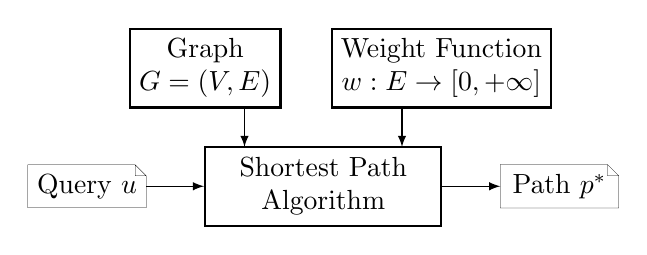
\begin{tikzpicture}
   \tikzset{>=latex} % arrow heads
   %\draw[step=1cm,black!10,very thin] (0,0) grid (8,4);
   \node[draw,align=center,minimum height=1.0cm,thick]
      at (2.5,2.5) {Graph\\$G=(V,E)$};
   \node[draw,align=center,minimum height=1.0cm,thick]
      at (5.5,2.5) {Weight Function\\$w:E \rightarrow [0,+\infty]$};
   \node[draw,align=center,minimum height=1.0cm,minimum width=3cm,thick]
      (alg) at (4,1) {Shortest Path\\Algorithm};
   \node[draw,align=center,shape=document,minimum width=1.5cm,ultra thin]
      (query) at (1,1) {Query $u$};
   \node[draw,align=center,shape=document,minimum width=1.5cm,ultra thin]
      (path) at (7,1) {Path $p^*$};
   \draw[->] (3,2) -- (3,1.5);
   \draw[->] (5,2) -- (5,1.5);
   \draw[->] (query.east) -- (alg.west);
   \draw[->] (alg.east) -- (path.west);
\end{tikzpicture}
\caption{While solving a shortest path query,
   a shortest path algorithm incurs computation cost from three sources:
   examining the structure of the graph $G$,
   evaluating the edge weight function $w$,
   and maintaining internal data structures.}
\label{fig:sp-intro}
\end{figure}

\section{The Shortest Path Problem}

Graphs provide a powerful abstraction
capable of representing problems in a wide variety of domains
from computer networking to puzzle solving
to robotic motion planning.
%\ajnote{Way too vague and general -- disconnected from second sentence.
%Maybe mention ``standard problems'' on graphs.}
In particular,
many important problems can be captured
as \emph{shortest path problems} (Figure~\ref{fig:sp-intro}),
wherein a path $p^*$ of minimal length is sought
between two query vertices through a graph $G$
with respect to an edge weight function $w$.
%As such,
%a large number of algorithms have been proposed in the literature
%for solving shortest path problems efficiently.

Despite the expansive applicability of this single abstraction,
there exist a wide variety of algorithms in the literature
for solving the shortest path problem efficiently.
%\ajnote{You say ``despite'' but the second part seems to follow from
%the first.
%There are many solutions because there are many problems.}
This is because the measure of computational efficiency,
and therefore the correct choice of algorithm,
is inextricably tied to the underlying problem domain.

The computational costs incurred by an algorithm
can be broadly categorized into three sources
corresponding to the blocks in Figure~\ref{fig:sp-intro}.
One such source consists of queries on the structure
of the graph $G$ itself.
The most commonly discussed such operation,
\emph{expanding} a vertex (determining its successors),
is especially fundamental
%\ajnote{especially costly?}
when the graph is represented implicitly,
e.g. for domains with large graphs
such as the 15-puzzle or Rubik's cube.
It is with respect to vertex expansions
that A* \citep{hart1968astar} is optimally efficient.

A second source of computational cost consists of maintaining
ordered data structures inside the algorithm itself,
which is especially important for problems with large branching
factors.
For such domains,
approaches such as partial expansion \citep{yoshizumi2000peastar}
or iterative deepening \citep{korf1985idastar}
significantly reduce the number of vertices generated and stored
by either selectively filtering surplus vertices from the frontier,
or by not storing the frontier at all.

The third source of computational cost arises not from reasoning
over the structure of $G$,
but instead from evaluating the edge weight function $w$
(i.e. we treat discovering an out-edge and determining its weight
separately).
Consider for example the problem of articulated robotic motion planning
using roadmap methods \citep{kavrakietal1996prm}.
While these graphs are often quite small
(fewer than $10^5$ vertices),
determining the weight of each edge requires performing many
collision and distance computations for the complex geometry
of the robot and environment,
resulting in planning times of multiple seconds to find a path.

As described in Chapter~\ref{chap:roadmaps},
we consider problem domains in which evaluating the edge weight
function $w$ dominates algorithm running time.
In this chapter,
we investigate the following research question:
\begin{quote}
{\normalsize
How can we minimize the number of edges we need to evaluate
to answer shortest-path queries?
}
\end{quote}

We make three primary contributions.
First,
inspired by lazy collision checking techniques from 
robotic motion planning \citep{bohlin2000lazyprm},
we formulate a class of shortest-path algorithms 
that is well-suited to problem domains with expensive edge evaluations.
Second,
we show that several existing algorithms in the literature
can be expressed as special cases of this algorithm.
Third,
we show that the extensibility afforded by the algorithm allows for
novel edge evaluation strategies,
which can outperform existing algorithms
over a set of example problems.

\section{Lazy Shortest Path Algorithm}

We describe a lazy approach to finding short paths
which is well-suited to domains with
expensive edge evaluations.

\subsection{Problem Definition}

A path $p$ in a graph $G = (V,E)$
is composed of a sequence of adjacent edges 
connecting two endpoint vertices.
Given an edge weight function
$w : E \rightarrow [0,+\infty]$,
the length of the path with respect to $w$ is then:
\begin{equation}
   \mbox{len}(p, w) = \sum_{e \in p} w(e).
   \label{eqn:lazysp:len-definition}
\end{equation}
Given a single-pair planning query
$u: (v_{\ms{start}}, \, v_{\ms{goal}})$
inducing a set of satisfying paths $P_u$,
the \emph{shortest-path problem} is:
\begin{equation}
   p^* = \argmin_{p \, \in \, P_u} \mbox{len}(p, w).
   \label{eqn:objective}
\end{equation}

A shortest-path algorithm computes a satisfying solution $p^*$
given $(G, u, w)$.
Many such algorithms have been proposed
to efficiently accommodate a wide array of underlying problem domains.
%(outlined in Section~\ref{sec:discussion}).
The well-known principle of best-first search (BFS)
is commonly employed to select vertices for expansion
so as to minimize such expansions while guaranteeing optimality.
Since we seek to minimize edge evaluations,
we apply BFS to the question of selecting candidate paths in
$G$ for evaluation.
The resulting algorithm, Lazy Shortest Path (LazySP),
is presented in Algorithm~\ref{alg:lazy-outline},
and can be applied to graphs defined implicitly or explicitly.

%\cdnote{To Sidd: You might not like this paragraph -- but I feel like
%going directly from the problem definition to the algorithm doesn't
%connect to the rationale strongly enough without it.
%What do you think?}

\subsection{The Algorithm}

\begin{algorithm}[t]
\caption{Lazy Shortest Path (LazySP)}
\label{alg:lazy-outline}
\begin{algorithmic}[1]
\Function {\textsc{LazyShortestPath}}{$G, u, w, w_{\ms{est}}$}
\State $E_{\ms{eval}} \leftarrow \emptyset$ %\Comment Initialize evaluated edges to empty
\State $w_{\ms{lazy}}(e) \leftarrow w_{\ms{est}}(e) \quad \forall e \in E$ %\Comment Initialize lazy edge weights to estimate (inexpensive)
\Loop
   \State $p_{\ms{candidate}} \leftarrow
      \mbox{\sc ShortestPath}(G, u, w_{\ms{lazy}})$ %\Comment Compute the shortest path with lazy edge weights
      \label{line:lazy-outline-shortestpath}
   \If {$p_{\ms{candidate}} \subseteq E_{\ms{eval}}$} %\Comment If all edges on path have already been evaluated,
      \State \Return $p_{\ms{candidate}}$ %\Comment path returned is provably optimal
   \EndIf
   \State $E_{\ms{selected}} \leftarrow  \mbox{\sc Selector}(G, p_{\ms{candidate}})$ %\Comment Select edges on path to process
   \label{line:lazy-outline-chooseedges} 
   \For {$e \in E_{\ms{selected}} \setminus E_{\ms{eval}}$} %\Comment For all unevaluated selected edges
      \State $w_{\ms{lazy}}(e) \leftarrow w(e)$ \Comment Evaluate (expensive)
      \State $E_{\ms{eval}} \leftarrow E_{\ms{eval}} \cup e$ %\Comment Add to evaluated edge set
   \EndFor
\EndLoop
\EndFunction
\end{algorithmic}
\end{algorithm}

We track evaluated edges with the set $E_{\ms{eval}}$.
We are given an estimator function $w_{\ms{est}}$ of the true edge weight $w$.
This estimator is inexpensive to compute
(e.g. edge length or even $0$).
We then define a \emph{lazy} weight function $w_{\ms{lazy}}$
which returns the
true weight of an evaluated edge and otherwise
uses the inexpensive estimator $w_{\ms{est}}$.

At each iteration of the search,
the algorithm uses $w_{\ms{lazy}}$ to compute a candidate path
$p_{\ms{candidate}}$
by calling an existing solver \textsc{ShortestPath}
(note that this invocation requires no evaluations of $w$).
Once a candidate path has been found,
it is returned if it is fully evaluated.
Otherwise,
an \emph{edge selector} is employed which selects
graph edge(s) for evaluation.
The true weights of these edges are then evaluated
(incurring the requisite computational cost),
and the algorithm repeats.

%\subsection{Theoretical Properties}

LazySP is complete and optimal:
\marginnote{Proof of all theorems are available
in Appendix~\ref{sec:appendix-proofs}.}

\begin{theorem}[Completeness of LazySP]
If the graph $G$ is finite,
\textsc{ShortestPath} is complete,
and the set $E_{\ms{selected}}$
returned by \textsc{Selector}
returns at least one unevaluated edge on $p_{\ms{candidate}}$,
then \textsc{LazyShortestPath} is complete.
\label{thm:lazy-completeness}
\end{theorem}

\begin{theorem}[Optimality of LazySP]
If $w_{\ms{est}}$ is chosen such that
$w_{\ms{est}}(e) \leq \epsilon \, w(e)$ for some parameter
$\epsilon \geq 1$ and
\textsc{LazyShortestPath} terminates
with some path $p_{\ms{ret}}$,
then $\mbox{len}(p_{\ms{ret}}, w) \leq \epsilon \, \ell^*$
with $\ell^*$ the length of an optimal path.
\label{thm:lazy-optimality}
\end{theorem}

The optimality of LazySP depends on the admissibility of
$w_{\ms{est}}$
in the same way that the optimality of A* depends on
the admissibility of its goal heuristic $h$.
Theorem~\ref{thm:lazy-optimality} establishes the general
bounded suboptimality of LazySP
w.r.t. the inflation parameter $\epsilon$.
While our theoretical results (e.g. equivalences)
hold for any choice of $\epsilon$,
for clarity our examples and experimental results
focus on cases with $\epsilon = 1$.

\subsection{The Edge Selector: Key to Efficiency}

\begin{algorithm}[t]
\caption{Various Simple LazySP Edge Selectors}
\begin{algorithmic}[1]
\Function {\textsc{SelectExpand}}{$G, p_{\ms{candidate}}$}
   \State $e_{\ms{first}} \leftarrow$ first unevaluated $e \in p_{\ms{candidate}}$
   \State $v_{\ms{frontier}} \leftarrow G.\mbox{source}(e_{\ms{first}})$
   \State $E_{\ms{selected}} \leftarrow G.\mbox{out\_edges}(v_{\ms{frontier}})$
   \State \Return $E_{\ms{selected}}$
\EndFunction
\vspace{0.02in}
\Function {\textsc{SelectForward}}{$G, p_{\ms{candidate}}$}
   \State \Return $\{ \mbox{first unevaluated } e \in p_{\ms{candidate}} \}$
\EndFunction
\vspace{0.02in}
\Function {\textsc{SelectReverse}}{$G, p_{\ms{candidate}}$}
   \State \Return $\{ \mbox{last unevaluated } e \in p_{\ms{candidate}} \}$
\EndFunction
\vspace{0.02in}
\Function {\textsc{SelectAlternate}}{$G, p_{\ms{candidate}}$}
   \If {LazySP iteration number is odd}
      \State \Return $\{ \mbox{first unevaluated } e \in p_{\ms{candidate}} \}$
   \Else
      \State \Return $\{ \mbox{last unevaluated } e \in p_{\ms{candidate}} \}$
   \EndIf
\EndFunction
\vspace{0.02in}
\Function {\textsc{SelectBisection}}{$G, p_{\ms{candidate}}$}
   \State \Return $\left\{ \begin{array}{ll}
      \mbox{unevaluated } e \in p_{\ms{candidate}} \\
      \mbox{furthest from nearest evaluated edge}
      \end{array} \right\}$
\EndFunction
\end{algorithmic}
\label{alg:simple-selectors}
\end{algorithm}

%The algorithm purposely leaves undecided
%the edge evaluation selector codified in
%\textsc{Selector} (line~\ref{line:lazy-outline-chooseedges}),
%and therefore describes a class of algorithms
%differentiated by the choice of this selector.
%This paper discusses particular choices.

The LazySP algorithm exhibits a rough similarity to optimal
replanning algorithms such as
D* \citep{stentz1994dstar,stentz1995focusseddstar}
which plan a sequence of shortest paths for a mobile robot
as new edge weights are discovered during its traverse.
D* treats edge changes
passively as an aspect of the problem setting
(e.g. a sensor with limited range).

The key difference is that our problem setting treats 
edge evaluations as an active choice that can be exploited.
While any choice of edge selector that meets the conditions above
will lead to an algorithm that is complete and optimal,
its \emph{efficiency} is dictated by the choice of this
selector.
This motivates the theoretical and empirical investigation of different
edge selectors in this chapter.

\textbf{Simple selectors.}
We codify five common strategies in
Algorithm~\ref{alg:simple-selectors}.
The Expand selector captures the edge weights that are evaluated
during a conventional vertex expansion.
The selector identifies the first unevaluated edge
$e_{\ms{first}}$ on the candidate path,
and considers the source vertex of this edge a \emph{frontier} vertex.
It then selects all out-edges of this frontier vertex
for evaluation.
The Forward and Reverse selectors select the first and last
unevaluated edge on the candidate path, respectively
(note that Forward returns a subset of Expand).

The Alternate selector simply alternates between Forward
and Reverse on each iteration.
This can be motivated by both bidirectional search algorithms
as well as motion planning algorithms such as
RRT-Connect \citep{kuffner2000rrtconnect}
which tend to perform well w.r.t. state evaluations.

The Bisection selector
chooses among those unevaluated edges
the one furthest from an evaluated edge on the candidate path.
This selector is roughly analogous to the collision checking strategy
employed by the Lazy PRM \citep{bohlin2000lazyprm}
as applied to our problem on abstract graphs.

In the following section,
we demonstrate that instances of LazySP using simple selectors
yield equivalent results to existing vertex algorithms.
We then discuss two more sophisticated
selectors motivated by weight function sampling
and statistical mechanics.

% prob-box2d00-halton-roots16
% fwd:34 partall:22 rev:24 fwdexpand:77
% bisect:25 worlddist:22 alt:23 partsimple:22
\begin{figure*}[t!]%
   \!\!%
   \subfloat[Expand(77)]{%
      \centering%
      \begin{tikzpicture}
         \node at (0,-0.0) {\includegraphics{build/lazysp-example-1/alg-fwdexpand-after5}};
         \node at (0,-2.5) {\includegraphics{build/lazysp-example-1/alg-fwdexpand-end}};
         \node at (0,-4.8) {\includegraphics{build/lazysp-example-1/alg-fwdexpand-path-bars}};
      \end{tikzpicture}%
   }%
   \!\!%
   \subfloat[Forward(34)]{%
      \centering%
      \begin{tikzpicture}
         \node at (0,-0.0) {\includegraphics{build/lazysp-example-1/alg-fwd-after5}};
         \node at (0,-2.5) {\includegraphics{build/lazysp-example-1/alg-fwd-end}};
         \node at (0,-4.8) {\includegraphics{build/lazysp-example-1/alg-fwd-path-bars}};
      \end{tikzpicture}%
   }%
   \!\!%
   \subfloat[Reverse(24)]{%
      \centering%
      \begin{tikzpicture}
         \node at (0,-0.0) {\includegraphics{build/lazysp-example-1/alg-rev-after5}};
         \node at (0,-2.5) {\includegraphics{build/lazysp-example-1/alg-rev-end}};
         \node at (0,-4.8) {\includegraphics{build/lazysp-example-1/alg-rev-path-bars}};
      \end{tikzpicture}%
   }%
   \!\!%
   \subfloat[Alternate(23)]{%
      \centering%
      \begin{tikzpicture}
         \node at (0,-0.0) {\includegraphics{build/lazysp-example-1/alg-alt-after5}};
         \node at (0,-2.5) {\includegraphics{build/lazysp-example-1/alg-alt-end}};
         \node at (0,-4.8) {\includegraphics{build/lazysp-example-1/alg-alt-path-bars}};
      \end{tikzpicture}%
   }%
   \!\!%
   \subfloat[Bisect(25)]{%
      \centering%
      \begin{tikzpicture}
         \node at (0,-0.0) {\includegraphics{build/lazysp-example-1/alg-bisect-after5}};
         \node at (0,-2.5) {\includegraphics{build/lazysp-example-1/alg-bisect-end}};
         \node at (0,-4.8) {\includegraphics{build/lazysp-example-1/alg-bisect-path-bars}};
      \end{tikzpicture}%
   }%
   \!\!%
   \subfloat[WeightSamp(22)]{%
      \centering%
      \begin{tikzpicture}
         \node at (0,-0.0) {\includegraphics{build/lazysp-example-1/alg-worlddist1000-after5}};
         \node at (0,-2.5) {\includegraphics{build/lazysp-example-1/alg-worlddist1000-end}};
         \node at (0,-4.8) {\includegraphics{build/lazysp-example-1/alg-worlddist1000-path-bars}};
      \end{tikzpicture}%
   }%
   \!\!%
   \subfloat[Partition(22)]{%
      \centering%
      \begin{tikzpicture}
         \node at (0,-0.0) {\includegraphics{build/lazysp-example-1/alg-partall-after5}};
         \node at (0,-2.5) {\includegraphics{build/lazysp-example-1/alg-partall-end}};
         \node at (0,-4.8) {\includegraphics{build/lazysp-example-1/alg-partall-path-bars}};
      \end{tikzpicture}%
   }%
   \caption[Snapshots of the LazySP algorithm using each edge selector
      discussed in this chapter on the same obstacle roadmap graph problem,
      with start and goal.
      At top, the algorithms after evaluating five edges
      (evaluated edges labeled as valid or invalid).
      At middle, the final set of evaluated edges.
      At bottom, for each unique path considered from left to right,
      the number of edges on the path that are
      already evaluated, evaluated and valid, evaluated and invalid,
      and unevaluated.
      The total number of edges evaluated is noted in brackets.
      Note that the scale on the Expand plot has been adjusted
      because the selector evaluates many edges not on the candidate
      path at each iteration.
   ]{Snapshots of the LazySP algorithm using each edge selector
      discussed in this chapter on the same obstacle roadmap graph problem,
      with start (\protect\tikz[baseline=-0.5ex]{\protect\node[circle,fill=blue,inner sep=1pt]{};})
      and goal (\protect\tikz[baseline=-0.5ex]{\protect\node[circle,fill=green,inner sep=1pt]{};}).
      At top, the algorithms after evaluating five edges
      (evaluated edges labeled as
      \protect\tikz{\protect\draw[very thick] (0,0) -- (0.15,0.15);}  valid
      or \protect\tikz{\protect\draw[very thick,red] (0,0) -- (0.15,0.15);} invalid).
      At middle, the final set of evaluated edges.
      At bottom, for each unique path considered from left to right,
      the number of edges on the path that are
      \protect\tikz{\protect\node[fill=green!40!white,draw=black]{};}\;already evaluated,
      \protect\tikz{\protect\node[fill=green!70!black,draw=black]{};}\;evaluated and valid,
      \protect\tikz{\protect\node[fill=red!70!black,draw=black]{};}\;evaluated and invalid,
      and \protect\tikz{\protect\node[fill=black!10!white,draw=black]{};}\;unevaluated.
      The total number of edges evaluated is noted in brackets.
      Note that the scale on the Expand plot has been adjusted
      because the selector evaluates many edges not on the candidate
      path at each iteration.
      }
   \label{fig:snapshots}
\end{figure*}

\section{Edge Equivalence to A* Variants}

In the previous section,
we introduced LazySP as the path-selection analogue
to BFS vertex-selection algorithms.
In this section,
we make this analogy more precise.
In particular,
we show that LazySP-Expand
%(that is, LazySP with the Expand selector)
%\ajnote{name consistency}
is edge-equivalent to a variant of A*
(and Weighted A*),
and that LazySP-Forward is edge-equivalent to a variant of
Lazy Weighted A*
(see Table~\ref{table:equivalences}).
%\ajnote{Say ``as described below''?}
It is important to be specific about the conditions under which
these equivalences arise,
which we detail here.

\begin{table}
   \centering
   {\small%
   \begin{tabular}{lll}
      \toprule
      LazySP & Existing & \\
      Selector & Algorithm & Result \\
      \midrule
      Expand & (Weighted) A* & Edge-equivalent \\
      & & (Theorems \ref{thm:astar-equiv-from-lazy},
                 \ref{thm:astar-equiv-to-lazy}) \\
      \addlinespace[0.3em]
      Forward & Lazy Weighted A* & Edge-equivalent \\
      & & (Theorems \ref{thm:lwastar-equiv-from-lazy},
                 \ref{thm:lwastar-equiv-to-lazy}) \\
      \addlinespace[0.3em]
      Alternate & Bidirectional Heuristic & Conjectured \\
      & Front-to-Front Algorithm & \\
      \bottomrule
   \end{tabular}%
   }%
   \caption{LazySP equivalence results.
      The A*, LWA*, and BHFFA algorithms use reopening and the dynamic
      $h_{\ms{lazy}}$ heuristic (\ref{eqn:h_lazy}).}
   \label{table:equivalences}
\end{table}

\textbf{Edge equivalence.}
We say that two algorithms are \emph{edge-equivalent} if they
evaluate the same edges in the same order.
We consider an algorithm to have evaluated an edge
the first time the edge's true weight is requested.

\textbf{Arbitrary tiebreaking.}
For some graphs,
an algorithm may have multiple allowable choices at each iteration
(e.g. LazySP with multiple shortest candidate paths,
or A* with multiple vertices in OPEN with lowest $f$-value).
We will say that algorithm A is equivalent to algorithm B
if for any choice available to A,
there exists an allowable choice available to B
such that the same edge(s) are evaluated by each.

\textbf{A* with reopening.}
We show equivalence to variants of A* and Lazy Weighted A*
that do not use a CLOSED list to prevent
vertices from being visited more than once.
%\ssnote{Why this comparison?! Not explained.}.
%Note that if the heuristic used is $h(v) = \epsilon h_c(v)$
%with $h_c(v)$ consistent,
%a CLOSED list could potentially reduce edge evaluations
%while still guaranteeing $\epsilon$-suboptimality.

\begin{figure}
   \centering
   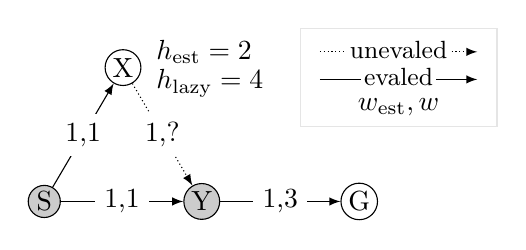
\begin{tikzpicture}
      \tikzset{>=latex} % arrow heads
      %\draw[step=1cm,black!10,very thin] (0,0) grid (8,4);
      \node[draw,circle,inner sep=1pt,fill=black!20] (S) at (1,1) {S};
      \node[draw,circle,inner sep=1pt] (X) at (2,2.7) {X};
      \node[draw,circle,inner sep=1pt,fill=black!20] (Y) at (3,1) {Y};
      \node[draw,circle,inner sep=1pt] (G) at (5,1) {G};
      \draw[->] (S) -- (Y) node [midway,fill=white] {1,1};
      \draw[->] (Y) -- (G) node [midway,fill=white] {1,3};
      \draw[->] (S) -- (X) node [midway,fill=white] {1,1};
      \draw[->,densely dotted] (X) -- (Y) node [midway,fill=white] {1,?};
      \node[anchor=west] at (2.3,2.9) {$h_{\ms{est}} = 2$};
      \node[anchor=west] at (2.3,2.5) {$h_{\ms{lazy}} = 4$};
      
      % for legend
      %\node at (7,2.9) {unevaluated:};
      %\draw[->,dashed] (6,2.5) -- (8,2.5)
      %   node [midway,fill=white] {($w_{est}$)\,?};
      %\node at (7,1.9) {evaluated:};
      %\draw[->] (6,1.5) -- (8,1.5)
      %   node [midway,fill=white] {($w_{est}$)\,$w$};
      \draw[->,densely dotted] (4.5,2.9) -- (6.5,2.9)
         node[midway,yshift=0.03cm,fill=white,inner sep=1pt,font=\small] {unevaled};
      \draw[->] (4.5,2.55) -- (6.5,2.55)
         node[midway,yshift=0.03cm,fill=white,inner sep=1pt,font=\small] {evaled};
      \node at (5.5,2.2) {$w_{\ms{est}},w$};
      \draw[black!10] (4.25,1.95) rectangle (6.75,3.2);
   \end{tikzpicture}
   \caption{A* comparison between
      the static goal heuristic $h_{\ms{est}}$ (\ref{eqn:h_est})
      and the dynamic goal heuristic $h_{\ms{lazy}}$ (\ref{eqn:h_lazy})
      on a simple graph from start S to goal G.
      The values of both the edge weight estimate $w_{\ms{est}}$
      and the true edge weight $w$ (for evaluated edges) are shown.
      Using either goal heuristic,
      the A* algorithm first expands vertices S and Y,
      evaluating three edges in total and leaving X and G on OPEN.
      After finding that edge YG has $w=3$,
      the dynamic heuristic value $h_{\ms{lazy}}(\mbox{X})$
      is updated from 2 to 4.
      While the A* using the static $h_{\ms{est}}$ would next expand X,
      the A* using the dynamic $h_{\ms{lazy}}$ would next expand G
      and terminate, having never evaluated edge XY.}
   \label{fig:updating-heuristic}
\end{figure}

\textbf{A* with a dynamic heuristic.}
In order to apply A* and Lazy Weighted A* to our problem,
we need a goal heuristic over vertices.
The most simple may be
\begin{equation}
   h_{\ms{est}}(v) = \min_{p : v \rightarrow v_g} \mbox{len}(p, w_{\ms{est}}).
   \label{eqn:h_est}
\end{equation}
Note that the value of this heuristic could be computed as a
pre-processing step using Dijkstra's algorithm \citep{dijkstra1959anote}
before iterations begin.
However,
in order for the equivalences to hold,
we require the use of the lazy heuristic
\begin{equation}
   h_{\ms{lazy}}(v) = \min_{p : v \rightarrow v_g} \mbox{len}(p, w_{\ms{lazy}}).
   \label{eqn:h_lazy}
\end{equation}
This heuristic is dynamic in that it depends on $w_{\ms{lazy}}$
which changes as edges are evaluated.
Therefore,
heuristic values must be recomputed for all affected vertices on OPEN
after each iteration.
%An illustrative example is shown in
%Figure~\ref{fig:updating-heuristic}.
%(We discuss efficient implementation of $h_{\ms{lazy}}$ as it relates
%to the D* family of algorithms in Section~\ref{sec:discussion}.)

\subsection{Equivalence to A*}

We show that the LazySP-Expand algorithm
is edge-equivalent to a variant of the A*
shortest-path algorithm.
%We consider the variant of A* which allows a vertex $v$ to be reopened
%if its stored cost $g[v]$ is improved.
We make use of two invariants that are maintained during the
progression of A*.
\marginnote{Proof of all invariants are available
in Appendix~\ref{sec:appendix-proofs}.}
\begin{invariant}
If $v$ is discovered by A* and $v'$ is undiscovered,
with $v'$ a successor of $v$,
then $v$ is on OPEN.%
\label{inv:astar-cundisc-popen}%
\end{invariant}
\begin{invariant}
If $v$ and $v'$ are discovered by A*,
with $v'$ a successor of $v$,
and $g[v] + w(v,v') < g[v']$,
then $v$ is on OPEN.%
\label{inv:astar-wless-popen}%
\end{invariant}
When we say a vertex is \emph{discovered},
we mean that it is either on OPEN or CLOSED.
Note that Invariant \ref{inv:astar-wless-popen} holds
because we allow vertices to be reopened;
without reopening (and with an inconsistent heuristic),
later finding a cheaper path to $v$ (and not reopening $v'$)
would invalidate the invariant.

We will use the goal heuristic $h_{\ms{lazy}}$ from (\ref{eqn:h_lazy}).
Note that if an admissible edge weight estimator $\hat{w}$ exists
(that is, $\hat{w} \leq w$),
then our A* can approximate the Weighted A* algorithm
\citep{pohl1970weightedastar}
with parameter $\epsilon$
by using $w_{\ms{est}} = \epsilon \, \hat{w}$,
and the suboptimality bound from
Theorem~\ref{thm:lazy-optimality} holds.

\begin{figure}[t]
   \centering
   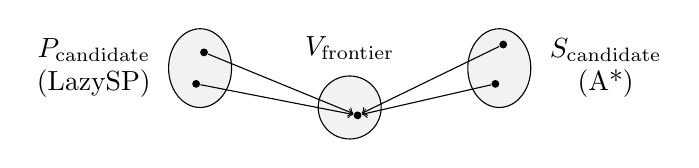
\begin{tikzpicture}
      %\draw[step=1cm,gray,very thin] (0,0) grid (8,3);
      
      \draw[fill=black!05] (2.1,1.5) ellipse (0.4cm and 0.5cm);
      \draw[fill=black!05] (5.9,1.5) ellipse (0.4cm and 0.5cm);
      \draw[fill=black!05] (4,1) ellipse (0.4cm and 0.4cm);
      
      \node[align=center] at (0.75,1.5) {$P_{\ms{candidate}}$\\(LazySP)};
      \node[align=center] at (7.25,1.5) {$S_{\ms{candidate}}$\\(A*)};
      \node[align=center] at (4,1.75) {$V_{\ms{frontier}}$};
      
      \node[fill=black,circle,inner sep=1pt] (p1) at (2.15,1.7) {};
      \node[fill=black,circle,inner sep=1pt] (p2) at (2.05,1.3) {};
      
      \node[fill=black,circle,inner sep=1pt] (s1) at (5.95,1.8) {};
      \node[fill=black,circle,inner sep=1pt] (s2) at (5.85,1.3) {};
      
      \node[fill=black,circle,inner sep=1pt] (v1) at (4.1,0.9) {};
      
      \draw[->] (p1) -- (v1);
      \draw[->] (p2) -- (v1);
      
      \draw[->] (s1) -- (v1);
      \draw[->] (s2) -- (v1);
      
   \end{tikzpicture}
   \caption{Illustration of the equivalence
      between A* and LazySP-Expand.
      After evaluating the same set of edges,
      the next edges to be evaluated by each algorithm
      can both be expressed as a surjective mapping onto
      a common set of unexpanded
      frontier vertices.
      }
   \label{fig:astar-equiv-mapping}
\end{figure}

\textbf{Equivalence.}
In order to show edge-equivalence,
we consider the case where both algorithms
are beginning a new iteration
having so far evaluated the same set of edges.

LazySP-Expand has some set $P_{\ms{candidate}}$ of allowable
candidate paths minimizing $\mbox{len}(p,w_{\ms{lazy}})$;
the Expand selector will then identify a vertex on the chosen path
for expansion.

A* will iteratively select a set of vertices from OPEN to expand.
Because it is possible that a vertex is expanded multiple times
(and only the first expansion results in edge evaluations),
we group iterations of A* into \emph{sequences},
where each sequence $s$ consists of
(a) zero or more vertices from OPEN that have already been expanded,
followed by (b) one vertex from OPEN that is to be expanded
for the first time.

We show that both the set of allowable candidate paths $P_{\ms{candidate}}$
available to LazySP-Expand
and the set of allowable candidate vertex sequences $S_{\ms{candidate}}$
available to A*
map surjectively to the same set of unexpanded frontier vertices $V_{\ms{frontier}}$
as illustrated in Figure~\ref{fig:astar-equiv-mapping}.
This is described by way of
Theorems \ref{thm:astar-equiv-from-lazy}
and \ref{thm:astar-equiv-to-lazy} below.
\marginnote{Proof of all theorems are available
in Appendix~\ref{sec:appendix-proofs}.}

\begin{theorem}
If LazySP-Expand and A* have evaluated the same set of edges,
then for any candidate path $p_{\ms{candidate}}$ chosen by LazySP
yielding frontier vertex $v_{\ms{frontier}}$,
there exists an allowable A* sequence $s_{\ms{candidate}}$
which also yields $v_{\ms{frontier}}$.
\label{thm:astar-equiv-from-lazy}
\end{theorem}

\begin{theorem}
If LazySP-Expand and A* have evaluated the same set of edges,
then for any candidate sequence $s_{\ms{candidate}}$ chosen by A*
yielding frontier vertex $v_{\ms{frontier}}$,
there exists an allowable LazySP path $p_{\ms{candidate}}$
which also yields $v_{\ms{frontier}}$.
\label{thm:astar-equiv-to-lazy}
\end{theorem}

\subsection{Equivalence to Lazy Weighted A*}

%\begin{algorithm}
%   \caption{Forward Edge Evaluation Selector}
%   \begin{algorithmic}[1]
%   \Function {\textsc{SelectForward}}{$G, p_{\ms{candidate}}$}
%   \State $e_{\ms{first}} \leftarrow$ first unevaluated $e \in p_{\ms{candidate}}$
%   \State \Return $\{ e_{\ms{first}} \}$
%   \EndFunction
%   \end{algorithmic}
%   \label{alg:selectforward}
%\end{algorithm}

In a conventional vertex expansion algorithm,
determining a successor's cost is a function of both
the cost of the edge and the value of the heuristic.
If either of these components is expensive to evaluate,
an algorithm can defer its computation by maintaining the successor
on the frontier with an approximate cost until it is expanded.
The Fast Downward algorithm \citep{helmert2006fastdownward} is motivated
by expensive heuristic evaluations in planning,
whereas the Lazy Weighted A* (LWA*) algorithm \citep{cohen2014narms}
is motivated by expensive edge evaluations in robotics.

We show that the LazySP-Forward algorithm
is edge-equivalent to a variant of the Lazy Weighted A*
shortest-path algorithm.
For a given candidate path,
the Forward selector returns the first unevaluated edge.

\textbf{Variant of Lazy Weighted A*.}
We reproduce a variant of LWA* without a CLOSED list
in Algorithm~\ref{alg:lwastar}.
For the purposes of our analysis,
the reproduction differs from the original presentation,
and we detail those differences here.
With the exception of the lack of CLOSED,
the differences do not affect the behavior of the algorithm.

\begin{algorithm}[t]
\caption{Lazy Weighted A* (without CLOSED list)}
\label{alg:lwastar}
\begin{algorithmic}[1]
\Function {\textsc{LazyWeightedA*}}{$G, w, \hat{w}, h$}
\State $g[v_{\ms{start}}] \leftarrow 0$
\State $Q_v \leftarrow \{ v_{\ms{start}} \}$
   \Comment Key: $g[v] + h(v)$
   \label{line:lwastar-key-qvertices}
\State $Q_e \leftarrow \emptyset$
   \Comment Key: $g[v] + \hat{w}(v,v') + h(v')$
   \label{line:lwastar-key-qedges}
\While {$\min(Q_v.{\mbox{TopKey}}, Q_e.{\mbox{TopKey}}) < g[v_{\ms{goal}}]$}
   \If {$Q_v.{\mbox{TopKey}} \leq Q_e.{\mbox{TopKey}}$}
      \State $v \leftarrow Q_v.{\mbox{Pop}}()$
      \For {$v' \in G.\mbox{GetSuccessors}(v)$}
         \State $Q_e.\mbox{Insert}((v,v'))$
      \EndFor
   \Else
      \State $(v,v') \leftarrow Q_e.{\mbox{Pop}}()$
      \If {$g[v'] \leq g[v] + \hat{w}(v,v')$}
         \label{line:lwastar-test}
         \State {\bf continue}
      \EndIf
      \State $g_{\ms{new}} \leftarrow g[v] + w(v,v')$
         \Comment evaluate
      \If {$g_{\ms{new}} < g[v']$}
         \State $g[v'] = g_{\ms{new}}$
         \State $Q_v.\mbox{Insert}(v')$
      \EndIf
   \EndIf
\EndWhile
\EndFunction
\end{algorithmic}
\end{algorithm}

The most obvious difference is that we present the original OPEN list
as separate vertex ($Q_v$) and edge ($Q_e$) priority queues,
with sorting keys shown on lines \ref{line:lwastar-key-qvertices}
and \ref{line:lwastar-key-qedges}.
A vertex $v$ in the original OPEN with $trueCost(v) = true$
corresponds to a vertex $v$ in $Q_v$,
whereas a vertex $v'$ in the original OPEN
with $trueCost(v') = false$ (and parent $v$)
corresponds to an edge $(v,v')$ in $Q_e$.
Use of the edge queue obviates the need for
duplicate vertices on OPEN with different parents
and the $conf(v)$ test for identifying such duplicates.
This presentation also highlights the similarity between LWA*
and the inner loop of the Batch Informed Trees (BIT*) algorithm
\citep{gammell2015bitstar}.

The second difference is that the edge usefulness test
(line 12 of the original algorithm)
has been moved from before inserting into OPEN
to after being popped from OPEN,
but before being evaluated
(line~\ref{line:lwastar-test} of Algorithm~\ref{alg:lwastar}).
This change is partially in compensation for removing the CLOSED
list.
This adjustment
does not affect the edges evaluated.

We make use of an invariant that is maintained during the
progression of Lazy Weighted A*.
\marginnote{Proof of all invariants are available
in Appendix~\ref{sec:appendix-proofs}.}
\begin{invariant}
For all vertex pairs $v$ and $v'$,
with $v'$ a successor of $v$,
if $g[v] + \max(w(v,v'), \hat{w}(v,v')) < g[v']$,
then either vertex $v$ is on $Q_{v}$
or edge $(v,v')$ is on $Q_e$.%
\label{inv:lwastar}%
\end{invariant}
We will use $h(v) = h_{\ms{lazy}}(v)$ from (\ref{eqn:h_lazy})
and $\hat{w} = w_{\ms{lazy}}$.
Note that the use of these dynamic heuristics requires that the
$Q_v$ and $Q_e$ be resorted after every edge is evaluated.

\textbf{Equivalence.}
The equivalence follows similarly to that for A* above.
Given the same set of edges evaluated,
the set of allowable next evaluations is identical for each
algorithm.
\marginnote{Proof of all theorems are available
in Appendix~\ref{sec:appendix-proofs}.}

\begin{theorem}
If LazySP-Forward and LWA* have evaluated the same set of edges,
then for any allowable candidate path $p_{\ms{candidate}}$
chosen by LazySP yielding first unevaluated edge $e_{ab}$,
there exists an allowable LWA* sequence $s_{\ms{candidate}}$
which also yields $e_{ab}$.
\label{thm:lwastar-equiv-from-lazy}
\end{theorem}

\begin{theorem}
If LazySP-Forward and LWA* have evaluated the same set of edges,
then for any allowable sequence of vertices and edges $s_{\ms{candidate}}$
considered by LWA* yielding evaluated edge $e_{ab}$,
there exists an allowable LazySP candidate path $p_{\ms{candidate}}$
which also yields $e_{ab}$.
\label{thm:lwastar-equiv-to-lazy}
\end{theorem}

\subsection{Relation to Bidirectional Heuristic Search}

LazySP-Alternate chooses unevaluated edges from either
the beginning or the end of the candidate path at each iteration.
We conjecture that an alternating version of the Expand selector
is edge-equivalent to the
Bidirectional Heuristic Front-to-Front Algorithm
\citep{champeauxsint1977bhffa}
for appropriate lazy vertex pair heuristic,
and that LazySP-Alternate is edge-equivalent
to a bidirectional LWA*.

\begin{algorithm}[t]
   \caption{Maximum Edge Probability Selector
      \emph{(for WeightSamp and Partition path distributions)}}
   \begin{algorithmic}[1]
   \Function {\textsc{SelectMaxEdgeProb}}{$G, p_{\ms{candidate}}, \mathcal{D}_p$}
   \State $p(e) \leftarrow \Pr( \, e \in P \, )
      \mbox{ for } P \sim \mathcal{D}_p$
   \State $e_{\ms{max}} \leftarrow$ unevaluated $e \in p_{\ms{candidate}}$
      maximizing $p(e)$
   \State \Return $\{ e_{\ms{max}} \}$
   \EndFunction
   \end{algorithmic}
   \label{alg:selectmaxscore}
\end{algorithm}

\section{Novel Edge Selectors}

Because we are conducting a search over paths,
we are free to implement selectors which are not constrained to
evaluate edges in any particular order
(i.e. to maintain evaluated trees rooted at the start and goal
vertices).
In this section,
we describe a novel class of edge selectors which is designed
to reduce the total number of edges evaluated during the course
of the LazySP algorithm.
These selectors operate by maintaining a distribution over potential
paths at each iteration of the algorithm
(see Figure~\ref{fig:maxprob-selectors-overview}).
This path distribution induces a Bernoulli distribution for each
edge $e$ which indicates its probability $p(e)$ to lie on
the potential path;
at each iteration,
the selectors then choose the unevaluated edge that maximizes
this edge indicator probability (Algorithm~\ref{alg:selectmaxscore}).
The two selectors described in this section differ
with respect to how they maintain this distribution over potential paths.

% make -f e8_experiments/scripts/Makefile.lazysp-fig-dists
\begin{figure}[t]
   \centering
   \begin{tikzpicture}
      \tikzset{>=latex}
      
      \node[draw,minimum width=2.4cm,minimum height=3.0cm] (startbox) at (-3.0,0) {};
      \node[inner sep=0pt] at (-3.0,-0.35) {\includegraphics[scale=2.0]{build/lazysp-fig-dists/fig-sofar}};
      \node[align=center,font=\small,below] at (startbox.north) {known\\edges};
      
      \node[draw] (quesbox) at (-1.2,0) {?};
      
      \node[draw,minimum width=2.1cm,minimum height=3.0cm] (pathsbox) at (0.4,0) {};
      \node[inner sep=0pt] at (-0.05, 0.1) {\includegraphics[scale=0.8]{build/lazysp-fig-dists/fig-path-00}};
      \node[inner sep=0pt] at ( 0.85, 0.1) {\includegraphics[scale=0.8]{build/lazysp-fig-dists/fig-path-01}};
      \node[inner sep=0pt] at (-0.05,-0.8) {\includegraphics[scale=0.8]{build/lazysp-fig-dists/fig-path-02}};
      \node[inner sep=0pt] at ( 0.85,-0.8) {\includegraphics[scale=0.8]{build/lazysp-fig-dists/fig-path-03}};
      \node[align=center,font=\small,below] at (pathsbox.north) {path\\distribution};
      \node[align=center,font=\normalsize,above] at (pathsbox.south) {$\dots$};
      
      \node[draw,minimum width=2.4cm,minimum height=3.0cm] (goalbox) at (3.0,0) {};
      \node[inner sep=0pt] at (3.0,-0.35) {\includegraphics[scale=2.0]{build/lazysp-fig-dists/fig-dist-probs}};
      \node[align=center,font=\small,below] at (goalbox.north) {edge indicator\\distributions};
      
      \draw[->] (startbox) -- (quesbox);
      \draw[->] (quesbox) -- (pathsbox);
      \draw[->] (pathsbox) -- (goalbox);
      
   \end{tikzpicture}
   \caption{Illustration of maximum edge probability selectors.
      A distribution over paths
      (usually conditioned on the known edge evaluations)
      induces on each edge $e$ a Bernoulli distribution
      with parameter $p(e)$
      giving the probability that it belongs to the path.
      The selector chooses the edge with the largest such probability.}
   \label{fig:maxprob-selectors-overview}
\end{figure}

\subsection{Weight Function Sampling Selector}

The first selector, WeightSamp,
is motivated by the intuition that it is preferable to evaluate edges
that are most likely to lie on the true shortest path.
Therefore,
it computes its path distribution $\mathcal{D}_p$
by performing shortest path queries
on sampled edge weight functions drawn from a distribution
$\mathcal{D}_w$.
This edge weight distribution is conditioned on the the known weights
of all previously evaluated edges $E_{\ms{eval}}$:
\begin{equation}
   \mathcal{D}_p : \mbox{SP}(w)
   \mbox{ for } w \sim \mathcal{D}_w(E_{\ms{eval}})
   \label{eqn:weightsamp}.
\end{equation}

For example,
the distribution $\mathcal{D}_w$ might consist of
the edge weights induced by a model of the distribution of
environment obstacles
(Figure~\ref{fig:weightsamp}).
Since this obstacle distribution is conditioned on the results
of known edge evaluations,
we consider the subset of worlds which are consistent
with the edges we have evaluated so far.
However,
depending on the fidelity of this model,
solving the corresponding shortest path problem for a given
sampled obstacle arrangement might require as much computation as
solving the original problem,
since it requires computing the resulting edge weights.
In practice,
we can approximate $\mathcal{D}_w$
by assuming that each edge is independently distributed.

\begin{figure}[t]
   \centering
   \begin{tikzpicture}
      \tikzset{>=latex}
      
      \node[draw,minimum width=1.8cm,minimum height=2.6cm] (startbox) at (-4.4,0) {};
      \node[inner sep=0pt] at (-4.4,-0.35) {\includegraphics[scale=1.5]{build/lazysp-fig-dists/fig-sofar}};
      \node[align=center,font=\small,below] at (startbox.north) {known\\edges};
      
      \node[draw,minimum width=1.8cm,minimum height=6cm] (abox) at (-2.2,0) {};
      \node[inner sep=0pt] at (-2.2, 1.3) {\includegraphics[scale=1.5]{build/lazysp-fig-dists/fig-world-00}};
      \node[inner sep=0pt] at (-2.2,-0.3) {\includegraphics[scale=1.5]{build/lazysp-fig-dists/fig-world-01}};
      \node[inner sep=0pt] at (-2.2,-1.9) {\includegraphics[scale=1.5]{build/lazysp-fig-dists/fig-world-02}};
      \node[align=center,font=\small,below] at (abox.north) {obstacle\\distribution};
      \node[align=center,font=\normalsize,above] at (abox.south) {$\dots$};
      
      \node[draw,minimum width=1.8cm,minimum height=6cm] (bbox) at (0,0) {};
      \node[inner sep=0pt] at (0, 1.3) {\includegraphics[scale=1.5]{build/lazysp-fig-dists/fig-wfn-00}};
      \node[inner sep=0pt] at (0,-0.3) {\includegraphics[scale=1.5]{build/lazysp-fig-dists/fig-wfn-01}};
      \node[inner sep=0pt] at (0,-1.9) {\includegraphics[scale=1.5]{build/lazysp-fig-dists/fig-wfn-02}};
      \node[align=center,font=\small,below] at (bbox.north) {weight fn\\distribution};
      \node[align=center,font=\normalsize,above] at (bbox.south) {$\dots$};
      
      \node[draw,minimum width=1.8cm,minimum height=6cm] (cbox) at (2.2,0) {};
      \node[inner sep=0pt] at (2.2, 1.3) {\includegraphics[scale=1.5]{build/lazysp-fig-dists/fig-path-00}};
      \node[inner sep=0pt] at (2.2,-0.3) {\includegraphics[scale=1.5]{build/lazysp-fig-dists/fig-path-01}};
      \node[inner sep=0pt] at (2.2,-1.9) {\includegraphics[scale=1.5]{build/lazysp-fig-dists/fig-path-02}};
      \node[align=center,font=\small,below] at (cbox.north) {path\\distribution};
      \node[align=center,font=\normalsize,above] at (cbox.south) {$\dots$};
      
      \draw[->] (startbox) -- (abox);
      \draw[->] (abox) -- (bbox);
      \draw[->] (bbox) -- (cbox);
   \end{tikzpicture}
   \caption{The WeightSamp selector uses the path distribution induced by
      solving the shortest path problem on a distribution over possible
      edge weight functions $\mathcal{D}_w$.
      In this example, samples from $\mathcal{D}_w$ are computed by
      drawing samples from $\mathcal{D}_O$,
      the distribution of obstacles that are consistent with
      the known edge evaluations.}
   \label{fig:weightsamp}
\end{figure}

\subsection{Partition Function Selector}

While the WeightSamp selector captures the intuition that it is
preferable to focus edge evaluations in areas that are useful for
many potential paths,
the computational cost required to calculate it at each iteration
may render it intractable.
One candidate path distribution that is more efficient to compute
follows an exponential form:
\begin{equation}
   \mathcal{D}_p : f_P(p) \propto
   \exp( - \beta \, \mbox{len}(p, w_{\ms{lazy}}) ).
\end{equation}
In other words,
we consider all potential paths $P$
between the start and goal vertices,
with shorter paths assigned more exponentially probability
than longer ones
(with positive parameter $\beta$).
We call this the Partition selector
because this distribution is closely related to calculating
partition functions from statistical mechanics.
The corresponding partition function is:
\begin{equation}
   Z(P) = \sum_{p \in P}
      \exp( - \beta \, \mbox{len}(p, w_{\ms{lazy}}) ).
   \label{eqn:partitionfn}
\end{equation}
Note that the edge indicator probability
required in Algorithm~\ref{alg:selectmaxscore}
can then be written:
\begin{equation}
   p(e) = 1 - \frac{Z(P \setminus e)}{Z(P)}.
   \label{eqn:edge-ind-prob}
\end{equation}
Here, $P \setminus e$ denotes paths in $P$ that do not
contain edge $e$.

\begin{figure}
   \centering
   \subfloat[Initial $p(e)$ scores on a constant-weight
         grid with $\beta$: 50, 33, 28]{%
      \centering
      \includegraphics{build/lazysp-selscores/empty-50}
      \includegraphics{build/lazysp-selscores/empty-33}
      \includegraphics{build/lazysp-selscores/empty-28}
      \label{subfig:partition-empty}
   }
   
   \subfloat[Initial $p(e)$ scores with $\infty$-weight
         obstacles with $\beta$: 50, 33, 28]{%
      \centering
      \includegraphics{build/lazysp-selscores/gap-50}
      \includegraphics{build/lazysp-selscores/gap-33}
      \includegraphics{build/lazysp-selscores/gap-28}
      \label{subfig:partition-passage}
   }
   
   % $ rosrun e8_experiments lazysp-partall-figure.py
   % --probdir=prob-box2d08-halton-roots12
   % --snapshot-afteredges=0 --out-tikz=partall-figure-0.tex
   \subfloat[Initial $p(e)$ scores]{%
      \centering
      \;
      \includegraphics{build/lazysp-partall/partall-figure-0}
      \;
      \label{subfig:partition-example-initial}
   }
   % $ rosrun e8_experiments lazysp-partall-figure.py
   % --probdir=prob-box2d08-halton-roots12
   % --snapshot-afteredges=5 --out-tikz=partall-figure-5.tex
   \subfloat[Scores after five evaluations]{%
      \centering
      \;
      \includegraphics{build/lazysp-partall/partall-figure-5}
      \;
      \label{subfig:partition-example-after5}
   }
   \vspace{0.2cm}

   \caption{Examples of the Partition selector's
      $p(e)$ edge score function.
      %(\subref{subfig:partition-empty})
      With no known obstacles,
      a high $\beta$ assigns near-unity score to only edges on the
      shortest path;
      as $\beta$ decreases and more paths are considered,
      edges immediately adjacent to the roots score highest.
      %(\subref{subfig:partition-passage})
      Since all paths must pass
      through the narrow passage,
      edges within score highly.
      %(\subref{subfig:partition-example-initial})
      For a problem with two a-priori known obstacles (dark gray),
      the score first prioritizes evaluations between the two.
      %(\subref{subfig:partition-example-after5})
      Upon finding these edges are blocked,
      the next edges that are prioritized lie along the top of the world.}
   \label{ref:example-scores}
\end{figure}

It may appear advantageous to restrict $P$ to only
\emph{simple} paths,
since all optimal paths are simple.
Unfortunately,
an algorithm for computing (\ref{eqn:edge-ind-prob}) efficiently is not
currently known in this case.
However,
in the case that $P$ consists of all paths,
there does exist an efficient incremental calculation of
(\ref{eqn:partitionfn}) via a recursive formulation.

We use the notation $Z_{xy} = Z(P_{xy})$,
with $P_{xy}$ the set of paths from $x$ to $y$.
Suppose the values $Z_{xy}$ are known between
all pairs of vertices $x, y$ for a graph $G$.
(For a graph with no edges,
$Z_{xy}$ is 1 if $x = y$ and 0 otherwise.)
Consider a modified graph $G'$ with one additional edge $e_{ab}$
with weight $w_{ab}$.
All additional paths use the new edge $e_{ab}$ a non-zero
number of times;
the value $Z'_{xy}$ can be shown to be
\begin{equation}
   Z'_{xy} = Z_{xy} + \frac{Z_{xa} Z_{by}}{\exp(\beta w_{ab}) - Z_{ba}}
   \mbox{ if }
   \exp(\beta w_{ab}) > Z_{ba}.
\end{equation}
This form is derived from simplifying the induced geometric series;
note that if $\exp(\beta w_{ab})  \leq Z_{ba}$,
the value $Z'_{xy}$ is infinite.
One can also derive the inverse:
given values $Z'$,
calculate the values $Z$ if an edge were removed.
A derivation of this formulation is given in
Appendix~\ref{chap:appendix-partition}.

This incremental formulation of (\ref{eqn:partitionfn})
allows for the corresponding score $p(e)$ for edges
to be updated efficiently during each iteration of LazySP as
the $w_{\ms{lazy}}$ value for edges chosen for evaluation are updated.
In fact,
if the values $Z$ are stored in a square matrix,
the update for all pairs after an edge weight change consists of a single
vector outer product.

\section{Experiments}

We compared the seven edge selectors on three classes of shortest path
problems.
The average number of edges evaluated by each,
as well as timing results from our implementations,
are shown in Figure~\ref{fig:results}.
In each case,
the estimate was chosen so that $w_{\ms{est}} \leq w$,
so that all runs produced optimal paths.
The experimental results serve primarily to illustrate that
the A* and LWA* algorithms
(i.e. Expand and Forward)
are not optimally edge-efficient,
but they also expose differences in behavior and prompt
future research directions.
All experiments were conducted using an open-source
implementation.
Motion planning results were implemented using
OMPL \citep{sucan2012ompl}.

\textbf{Random partially-connected graphs.}
We tested on a set of 1000 randomly-generated undirected graphs
with $|V|=100$,
with each pair of vertices sharing an edge with probability 0.05.
Edges have an independent 0.5 probability of having infinite weight,
else the weight is uniformly distributed on $[1,2]$;
the estimated weight was unity for all edges.
For the WeightSamp selector,
we drew 1000 $w$ samples.
For the Partition selector, we used $\beta = 2$.

\textbf{Roadmap graphs on the unit square.}
We considered roadmap graphs formed via the first 100 points
of the $(2,3)$-Halton sequence on the unit square
with a connection radius of 0.15,
with 30 pairs of start and goal vertices chosen randomly.
The edge weight function was derived from 30 sampled obstacle fields
consisting of 10 randomly placed boxes
with dimensions uniform on $[0.1,0.3]$,
with each edge having infinite weight on collision,
and weight equal to its Euclidean length otherwise.
One of the resulting 900 example problems is shown in
Figure~\ref{fig:snapshots}.
For the WeightSamp selector,
we drew 1000 $w$ samples
with a na\"{\i}ve edge weight distribution in which
each edge had an independent 0.1 collision probability.
For the Partition selector, we used $\beta = 21$.

\textbf{Roadmap graphs for robot arm motion planning.}
We considered roadmap graphs in the configuration space
corresponding to 7-DOF right arm of the HERB home robot across three
motion planning problems inspired by a table clearing scenario
(see Figure~\ref{fig:herbbin0}).
The problems consisted of first moving from the robot's
home configuration to one of 7 feasible grasp configurations for a mug
(pictured),
second transferring the mug to one of 72 feasible configurations with
the mug above the blue bin,
and third returning to the home configuration.
Each problem was solved independently.
This common scenario spans various numbers of starts/goals
and allows a comparison w.r.t. difficulty at different problem
stages as discussed later.

For each problem,
50 random graphs were constructed by applying a random offset to
the 7D Halton sequence with $N = 1000$,
with additional vertices for each problem start and goal configuration.
We used an edge connection radius of 3 rad,
resulting $|E|$ ranging from 23404 to 28109.
Each edge took infinite weight on collision,
and weight equal to its Euclidean length otherwise.
For the WeightSamp selector,
we drew 1000 $w$ samples
with a na\"{\i}ve edge weight distribution in which
each edge had an independent 0.1 probability of collision.
For the Partition selector, we used $\beta = 3$.

\begin{figure*}
\centering
%\includegraphics[width=3cm]{figs/herbbin0.png}
\includegraphics[width=3.1cm]{figs/lazysp-herbarm/herbarm-roadmap.png}
\includegraphics[width=3.1cm]{figs/lazysp-herbarm/herbarm-path02.png}
%\includegraphics[width=3cm]{figs/lazysp-herbarm/herbarm-path11.png}
%\includegraphics[width=3cm]{figs/lazysp-herbarm/herbarm-path21.png}
\includegraphics[width=3.1cm]{figs/lazysp-herbarm/herbarm-path33.png}
\includegraphics[width=3.1cm]{figs/lazysp-herbarm/herbarm-path42.png}
\includegraphics[width=3.1cm]{figs/lazysp-herbarm/herbarm-path46.png}
\caption{Visualization of the first of three articulated motion
   planning problems in which the HERB robot must move its right arm
   from the start configuration (pictured)
   to any of seven grasp configurations for a mug.
   Shown is the progression of the Alternate selector on one of the
   randomly generated roadmaps;
   approximately 2\% of the 7D roadmap is shown in gray by projecting
   onto the space of end-effector positions.}
\label{fig:herbbin0}
\end{figure*}

\begin{figure}[t!]
   \centering
   \subfloat[
      Average number of edges evaluated for each problem class
         and selector.
         The minimum selector,
         along with any selector within one unit of its standard error,
         is shown in bold.
         The ArmPlan class is split into its three constituent problems.
         Online timing results are also shown,
         including the components from the invoking the selector
         and evaluating edges.
         \dag PartConn and UnitSquare involve trivial edge evaluation
         time.
         \ddag Timing for the Partition selector does not include
         pre-computation time.
         See Figure~\ref{fig:table-timing-results} for details.]
   {%
      \centering
      {\small%
      \setlength{\tabcolsep}{0.06cm}%
      \begin{tabular}{lrrrrrrr}
         \toprule
            & E\;\;\;\;
            & F\;\;\;\; & R\;\;\;\; & A\;\;\;\;
            & B\;\;\;\; & W\;\;\;\; & P\ddag\;\; \\
         \midrule
         \addlinespace[0.3em]
         PartConn &  87.10 & 35.86 & 34.84 & 22.23 & 44.81 & \textbf{20.66} & \textbf{20.39} \\
         \;\;\emph{online\dag (ms)} & \bf\emph{1.22} & \emph{1.96} & \emph{1.86} & \bf\emph{1.20} & \emph{2.41} & \emph{4807.19} & \emph{3.32} \\
         \;\;\;\;\emph{sel (ms)} & \emph{0.02} & \emph{0.01} & \emph{0.01} & \emph{0.01} & \emph{0.03} & \emph{4805.64} & \emph{2.07} \\
         \addlinespace[0.3em]
         UnitSquare &  69.21 & 27.29 & 27.69 & 17.82 & 32.62 & 15.58 & \textbf{14.08} \\
         \;\;\emph{online\dag (ms)} & \bf\emph{0.91} & \emph{1.47} & \emph{1.49} & \bf\emph{0.94} & \emph{1.71} & \emph{3864.95} & \emph{1.72} \\
         \;\;\;\;\emph{sel (ms)} & \emph{0.01} & \emph{0.01} & \emph{0.01} & \emph{0.01} & \emph{0.02} & \emph{3863.49} & \emph{0.87} \\
         \addlinespace[0.3em]
         ArmPlan(avg) & 949.05 & 63.62 & 74.94 & 55.48 & 68.01 & 56.93 & \textbf{48.07} \\
         \;\;\emph{online (s)} & \emph{269.82} & \bf\emph{5.90} & \emph{8.22} & \bf\emph{5.96} & \emph{7.34} & \emph{3402.21} & \bf\emph{5.80} \\
         \;\;\;\;\emph{sel (s)} & \emph{0.00} & \emph{0.00} & \emph{0.00} & \emph{0.00} & \emph{0.00} & \emph{3392.76} & \emph{1.54} \\
         \;\;\;\;\emph{eval (s)} & \emph{269.78} & \emph{5.87} & \emph{8.20} & \emph{5.94} & \emph{7.31} & \emph{9.39} & \emph{4.21} \\
         \addlinespace[0.3em]
         ArmPlan1 &  344.74 & \textbf{49.72} & 95.58 & 59.44 & 58.90 & 73.72 & \textbf{50.66} \\
         \;\;\emph{online (s)} & \emph{109.09} & \bf\emph{4.81} & \emph{14.81} & \emph{7.03} & \emph{7.91} & \emph{3375.35} & \emph{7.25} \\
         \;\;\;\;\emph{sel (s)} & \emph{0.00} & \emph{0.00} & \emph{0.00} & \emph{0.00} & \emph{0.00} & \emph{3358.82} & \emph{1.61} \\
         \;\;\;\;\emph{eval (s)} & \emph{109.07} & \emph{4.78} & \emph{14.77} & \emph{7.01} & \emph{7.88} & \emph{16.47} & \emph{5.59} \\
         \addlinespace[0.3em]
         ArmPlan2 &  657.02 & \textbf{62.24} & 98.54 & 69.96 & 75.88 & \textbf{66.24} & \textbf{62.16} \\
         \;\;\emph{online (s)} & \emph{166.19} & \bf\emph{3.27} & \emph{7.36} & \emph{5.95} & \emph{5.63} & \emph{4758.04} & \emph{5.99} \\
         \;\;\;\;\emph{sel (s)} & \emph{0.00} & \emph{0.00} & \emph{0.00} & \emph{0.00} & \emph{0.00} & \emph{4750.16} & \emph{2.03} \\
         \;\;\;\;\emph{eval (s)} & \emph{166.17} & \emph{3.26} & \emph{7.34} & \emph{5.93} & \emph{5.61} & \emph{7.82} & \emph{3.91} \\
         \addlinespace[0.3em]
         ArmPlan3 & 1845.38 & 78.90 & \textbf{30.70} & 37.04 & 69.26 & \textbf{30.82} & \textbf{31.38} \\
         \;\;\emph{online (s)} & \emph{534.16} & \emph{9.61} & \bf\emph{2.50} & \emph{4.91} & \emph{8.47} & \emph{2073.23} & \emph{4.17} \\
         \;\;\;\;\emph{sel (s)} & \emph{0.00} & \emph{0.00} & \emph{0.00} & \emph{0.00} & \emph{0.00} & \emph{2069.29} & \emph{0.98} \\
         \;\;\;\;\emph{eval (s)} & \emph{534.10} & \emph{9.58} & \emph{2.48} & \emph{4.89} & \emph{8.44} & \emph{3.90} & \emph{3.15} \\
         \addlinespace[0.15em]
         \bottomrule
      \end{tabular}%
      }%
      \label{subfig:table-results}
   }
   
   \vspace{0.1in}
   
   \subfloat[PartConn]{%
      \centering
      \begin{tikzpicture}
      \begin{axis}[
         width=4.1cm,
         height=4.0cm,
         ybar,
         bar width=7,
         ymin=0,ymax=90,
         ytick pos=bottom,
         symbolic x coords={E, F, R, A, B, W, P},
         xtick=data,
         xtick pos=left,
         ymajorgrids,
         ymajorticks=false,
         ticklabel style={font=\small}
         ]
      \node[circle,fill=white,inner sep=1pt,text=black!40] at (axis cs:P,40) {\scriptsize 40};
      \node[circle,fill=white,inner sep=1pt,text=black!40] at (axis cs:P,60) {\scriptsize 60};
      \node[circle,fill=white,inner sep=1pt,text=black!40] at (axis cs:P,80) {\scriptsize 80};
      \addplot[color=black,fill=black!20,error bars/.cd,y dir=both,y explicit] coordinates {
         (E, 87.10) +- (2.39,2.39)
         (F, 35.86) +- (1.04,1.04)
         (R, 34.84) +- (1.04,1.04)
         (A, 22.23) +- (0.60,0.60)
         (B, 44.81) +- (1.11,1.11)
         (W, 20.66) +- (0.57,0.57)
         (P, 20.39) +- (0.56,0.56)
      };
      \end{axis}
      \end{tikzpicture}
   }
   \subfloat[UnitSquare]{%
      \centering
      \begin{tikzpicture}
      \begin{axis}[
         width=4.1cm,
         height=4.0cm,
         ybar,
         bar width=7,
         ymin=0,ymax=90,
         ytick pos=bottom,
         symbolic x coords={E, F, R, A, B, W, P},
         xtick=data,
         xtick pos=left,
         ymajorgrids,
         ymajorticks=false,
         ticklabel style={font=\small}
         ]
      \node[circle,fill=white,inner sep=1pt,text=black!40] at (axis cs:P,40) {\scriptsize 40};
      \node[circle,fill=white,inner sep=1pt,text=black!40] at (axis cs:P,60) {\scriptsize 60};
      \node[circle,fill=white,inner sep=1pt,text=black!40] at (axis cs:P,80) {\scriptsize 80};
      \addplot[color=black,fill=black!20,error bars/.cd,y dir=both,y explicit] coordinates {
         (E, 69.21) +- (2.55,2.55)
         (F, 27.29) +- (1.03,1.03)
         (R, 27.69) +- (1.02,1.02)
         (A, 17.82) +- (0.60,0.60)
         (B, 32.62) +- (0.72,0.72)
         (W, 15.58) +- (0.47,0.47)
         (P, 14.08) +- (0.46,0.46)
      };
      \end{axis}
      \end{tikzpicture}
   }
   \subfloat[ArmPlan]{%
      \centering
      \begin{tikzpicture}
      \begin{axis}[
         width=4.1cm,
         height=4.0cm,
         ybar,
         bar width=7,
         ymin=0,ymax=115,
         max space between ticks=10,
         ytick pos=bottom,
         symbolic x coords={E, F, R, A, B, W, P},
         xtick=data,
         xtick pos=left,
         ymajorgrids,
         ymajorticks=false,
         ticklabel style={font=\small}
         ]
      \node[circle,fill=white,inner sep=0pt,text=black!40] at (axis cs:P,60) {\scriptsize 60};
      \node[circle,fill=white,inner sep=0pt,text=black!40] at (axis cs:P,80) {\scriptsize 80};
      \node[circle,fill=white,inner sep=0pt,text=black!40] at (axis cs:P,100) {\scriptsize 100};
      \addplot[color=black,fill=black!20,error bars/.cd,y dir=both,y explicit] coordinates {
         (E, 115) +- (0,0) % 49.06 +- 61.63.46
         (F, 63.62) +- (4.15,4.15)
         (R, 74.94) +- (5.07,5.07)
         (A, 55.48) +- (2.95,2.95)
         (B, 68.01) +- (3.86,3.86)
         (W, 56.93) +- (3.37,3.37)
         (P, 48.07) +- (2.44,2.44)
      };
      \node[align=center,anchor=north,inner sep=0pt] at (axis cs:E,111) {\scriptsize $\uparrow$};
      \end{axis}
      \end{tikzpicture}
   }
   \caption{
      Experimental results for the three problem classes
      across each of the seven selectors,
      E:Expand, F:Forward, R:Reverse,
      A:Alternate, B:Bisection,
      W:WeightSamp, and P:Partition.
      In addition to the summary table (a),
      the plots (b-d) show summary statistics for
      each problem class.
      The means and standard errors in (b-c) are across the
      1000 and 900 problem instances, respectively.
      The means and standard errors in (d) are for
      the average across the three constituent problems
      for each of the 50 sampled roadmaps.
      A more detailed table of results is available
      in Appendix~\ref{sec:appendix-proofs}.}
   \label{fig:results}
\end{figure}

\section{Discussion}
%\label{sec:discussion}

The first observation that is evident from the experimental results
is that lazy evaluation
-- whether using Forward (LWA*) or one of the other selectors --
grossly outperforms Expand (A*).
The relative penalty that Expand incurs by evaluating all edges from
each expanded vertex is a function of the graph's branching factor.

Since the Forward and Reverse selectors are simply mirrors of each
other,
they exhibit similar performance
averaged across the PartConn and UnitSquare problem classes,
which are symmetric.
However,
this need not the case for a particular instance.
For example,
the start of ArmPlan1 and the goal of ArmPlan3 consist
of the arm's single home configuration in a relatively confined space.
As shown in the table in
Figure~\ref{fig:results}\subref{subfig:table-results},
it appears that the better selector on these problems attempts
to solve the more constrained side of the problem first.
While it may be difficult to determine a priori which part of the
problem will be the most constrained,
the simple Alternate selector's respectable performance
suggests that it may be a reasonable compromise.

The per-path plots at the bottom of Figure~\ref{fig:snapshots}
allow us to characterize the selectors' behavior.
For example,
Alternate often evaluates several edges on each path before finding
an obstacle.
Its early evaluations also tend to be useful later,
and it terminates after considering 10 paths on the illustrated problem.
In contrast, Bisection exhibits a fail-fast strategy,
quickly invalidating most paths after a single evaluation,
but needing 16 such paths (with very little reuse)
before it terminates.
In general, the Bisection selector did not outperform any of the
lazy selectors in terms of number of edges evaluated.
However,
it may be well suited to problem domains in which
evaluations that fail tend be less costly.

The novel selectors based on path distributions tend to minimize
edge evaluations on the problems we considered.
While the WeightSamp selector performs similarly to Partition on the
simpler problems,
it performs less well in the ArmPlan domain.
This may be because many more samples are needed to approximate
the requisite path distribution.

The path distribution selectors are motivated by focusing evaluation
effort in areas that are useful for many distinct candidate paths,
as illustrated in Figure~\ref{ref:example-scores}.
Note that in the absence of a priori knowledge,
the edges nearest to the start and goal tend to have the highest
$p(e)$ score,
since they are members of many potential paths.
Because it tends to focus evaluations in a similar way,
the Alternate selector may serve as a simple proxy for the
more complex selectors.

We note that
an optimal edge selector could be theoretically achieved by posing the
edge selection problem as a POMDP,
given a probabilistic model of the true costs.
While likely intractable in complex domains,
exploring this solution may yield useful approximations or insights.

\chapter{Efficient Incremental Search}
\label{chap:ibid}

In Chapter~\ref{chap:lazysp},
we introduced the Lazy Shortest Path (LazySP) algorithm,
which addresses domains with expensive edge weight functions
by interleaving the evaluation phase with a sequence of 
search queries using an existing pathfinding algorithm.
Because this inner search is conducted many times,
its efficiency is paramount.

Most approaches for reducing the computational cost of pathfinding
attempt to focus the search on a smaller subset of the graph.
We consider three classes of such techniques
(Figure~\ref{fig:ibid:intro-focus}):

\begin{marginfigure}[5cm]%
   \centering%
   \subfloat[Bidirectional search.]{%
      \centering %
      \includegraphics{build/ibid-intro-focus-bidirectional} %
   }%
   
   \subfloat[Heuristic search.]{%
      \centering %
      \includegraphics{build/ibid-intro-focus-heuristic} %
   }%
   
   \subfloat[Incremental search. \ssnote{hard to follow}]{%
      \centering %
      \includegraphics{build/ibid-intro-focus-incremental} %
   }%
   
   \caption{Illustrations of the three focusing techniques considered
      on a spatial pathfinding problem.}%
   \label{fig:ibid:intro-focus}
\end{marginfigure}

\begin{enumerate}
\item \emph{Bidirectional Search} -- A bidirectional algorithm
   conducts two concurrent searches,
   one from the source vertex $s$,
   and the other from the sink vertex $t$.
   Such searches are well-suited to roadmaps in ambient spaces that
   are high-dimensional \ssnote{how does this translate to number of nodes
   or edges or degree?} and/or have
   obstacles situated close to the source/sink vertices
   \ssnote{hmm, isn't bidirectional Djikstra best when the searches
   meet in the middle, so won't it expand a lot more nodes if sources
   or sinks are harder when compared to both being equally hard?}.
\item \emph{Heuristic Search} -- A heuristic-informed algorithm
   exploits a sink-directed heuristic function over vertices to bias
   exploration in the direction of the sink vertex.
   A strong and admissible such heuristic can drastically speed the
   search, \ssnote{might want to specify exactly how, i.e. expanding
   fewer vertices}
   although the efficacy is reduced for weaker heuristics.
\item \emph{Incremental Search} -- An incremental algorithm
   is applied to a sequence of search queries on a graph whose
   edge weight function changes (partially) between queries.
   \ssnote{isn't this a bit too specific?
   doesn't it also apply to cases where the vertex topology changes?}
   It endeavors to only consider the portion of its data structure
   affected by the changes. \ssnote{might want to say that it's called
   \emph{incremental} because it incrementally updates only the portion
   of the data structure that is relevant for solving the problem.}
\end{enumerate}

The principal contribution of this chapter is IBiD,
an algorithm which combines these three techniques into a single
algorithm
(Table~\ref{tab:ibid:alg-overview}).
While originally motivated for use with LazySP,
IBiD is broadly applicable to incremental search problems.

\paragraph{Chapter outline.}
Finding shortest paths on graphs is a very extensively studied problem.
This chapter begins with a comprehensive review of 
methods which solve shortest path problems by computing
distance functions.
After defining the problem in Section~\ref{subsec:ibid-probdef},
we review distance functions and unidirectional methods
in Section~\ref{sec:ibid:distance-functions}.
Section~\ref{sec:ibid:bidirectional} reviews
bidirectional search methods,
and Section~\ref{sec:ibid:incremental} reviews incremental search.
Section~\ref{sef:ibid:ibid}, introduces IBiD,
an algorithm which combines bidirectional and incremental search.
In Section~\ref{sec:ibid:heuristic},
we review heuristic search methods,
and discuss a heuristic-informed generalization of IBiD.
The chapter concludes with experimental results and implentation notes.

\begin{table}
   \centering
   \begin{tabular}{ccc}
      \toprule
      & Unidirectional & Bidirectional \\
      \midrule
      \addlinespace[0.2em]
      Complete
         & Dijkstra \citep{dijkstra1959anote}
         & Bidirectional Dijkstra \citep{luby1989bidijk} \\
      \addlinespace[-0.2em]
      \emph{(Heuristic)}
         & \emph{A* \citep{hart1968astar}}
         & \emph{Bidirectional A* \citep{ikeda1994betterroutes}} \\
      \addlinespace[0.3em]
      Incremental
         & DynamicSWSF-FP \citep{ramalingam1996dynamicswsffp}
         & {IBiD} \\
      \addlinespace[-0.2em]
      \emph{(Heuristic)}
         & \emph{Lifelong Planning A* \citep{koenig2004lpastar}}
         & \emph{Heuristic IBiD} \\
      \addlinespace[0.2em]
      \bottomrule
   \end{tabular}
   \caption{
      IBiD generalizes both the heuristic-informed
      bidirectional Dijkstra's search \citep{goldberg2005spexternalmemory}
      and DynamicSWSF-FP \citep{ramalingam1996dynamicswsffp}.
      There are a great many algorithms that we could place in each cell;
      we provide only a represetative choice in each.}
   \label{tab:ibid:alg-overview}
\end{table}

\section{Problem Definition}
\label{subsec:ibid-probdef}

The \emph{shortest path problem} on graphs has been extensively
studied over the past six decades.
Consider a directed graph $G = (V,E)$ and accompanying edge weight
function $w : E \rightarrow \mathbb{R}$.
Note that we allow graphs with multiple edges connecting any pair
of vertices,
as well as graphs with edges to and from the same vertex.

The length of a path is equal to the sum of the weights of its
constituent edges.
\marginnote{
The single-pair problem is also called the \emph{two-terminal} or
\emph{point-to-point} problem.}
We consider the \emph{single-pair shortest path} (SPSP) problem,
in which a path of minimal length is sought
between distinct start and destination vertices
$s,t \in V$.
(We can also handle planning problems with multiple
start/goal configurations as an SPSP problem
as described in Section~\ref{subsec:roadmaps:planning-as-pathfinding}.)

Our review is applicable to problems where $w$ is everywhere finite.
The algorithms that we consider do not distinguish between non-existant
and infinite-weight edges,
and so will return that no path exists in the case where shortest
paths contain infinite-weight edges.

\paragraph{An example problem.}
\begin{marginfigure}%
   \centering%
   \begin{tikzpicture}
      \tikzset{>=latex} % arrow heads
      \node[inner sep=0pt,anchor=south west] {%
         \includegraphics[width=5cm]{figs/incbi-road-ne/singleshot/example-intro.png}};
      \coordinate (s) at (1.75,0.9);
      \coordinate (t) at (3.93,2.8);
      \node (slab) at (2.5,0.6) {$s$};
      \node (tlab) at (4.0,1.5) {$t$};
      \draw[->,thick] (slab) -- (s);
      \draw[->,thick] (tlab) -- (t);
   \end{tikzpicture}%
   \caption{A graph of the Northeast USA from the 9th DIMACS
      Implementation Challenge
      comprises 1,524,453 vertices and 3,868,020 directed edges.
      A shortest path problem from a source $s$ in New Jersey
      to a target $t$ outisde Boston
      will be used as an example.}%
   \label{fig:ibid:example-intro}%
\end{marginfigure}
We will carry forward an illustrative example problem from
the public dataset of the 9th DIMACS Implementation Challenge
\citep{demetrescuetal2006dimacs9}
(Northeast USA)
comprising an approximate road network,
using transit time as the edge weight function
(Figure~\ref{fig:ibid:example-intro}).
In this way,
a shortest path between a pair of start and destination locations
minimizes the total transit time between them.
\ssnote{Might want to provide 1-2 sentence intuition on why
this graph is interesting, and why we chose it for IBID. 
High degree? Nonuniform degree?
Large variation in edge weights?}

\paragraph{Problem Settings.}
The single-pair problem has been extensively studied.
There are techniques that are particular to memory-constrained
settings \citep{kaindl1997biheurreconsidered}
or to settings where pre-computation is available
\citep{goldberg2007pointtopoint}.
While we do not focus on such settings,
the algorithms we propose may be complementary to these techniques.

\section{Review of Pathfinding with Distance Functions}
\label{sec:ibid:distance-functions}

This section contains a unified presentation of unidirectional,
bidirectional, and incremental search stategies
by examining the properties of the distance functions that they
maintain.
These properties and invariants can be established for arbitrary
distance function approximations.
Examination of these properties then informs the development of
algorithms which calculate them,
which we defer to Section~\ref{sef:ibid:ibid}.

While much of this section summaries prior work,
the presentation of the bidirectional termination condition
(Theorem~\ref{thm:ibid-bidir-sound}
in Section~\ref{sec:ibid:bidirectional})
in particular
is formulated to enable the novel theorems
presented in Section~\ref{sef:ibid:ibid}.

\subsection{Shortest Paths via the Source Distance Function}

The pioneering pathfinding algorithms of the late 1950s address
a generalization of the SPSP problem called
the \emph{single-source} problem,
where shortest paths are calculated from the start vertex $s$
to all vertices on the graph.
They proceed by calculating the \emph{source distance function}
$d^* : V \rightarrow \mathbb{R}$,
which gives the length of the shortest path from $s$
to each vertex $v$.
In other words:
\marginnote{Once the distance function $d^*$ is computed,
a shortest path to any target $t$ can be generated trivially
by walking backwards to $s$ guided by $d^*$.}
\begin{equation}
   d^*(v) = \min_{p \in P_{sv}} \mbox{len}(p),
   \label{eqn:ibid-distance-function-global}
\end{equation}
where $P_{sv}$ is the set of all paths from $s$ to $v$.
\ssnote{Have you defined len elsewhere? If so, provide pointer.
Is it meant to be the sum of weights along the path?
\begin{equation}
   d^*(v) = \min_{p \in P_{sv}} \mbox{len}(p) = \min_{p \in P_{sv}} \sum_{e \in p} w(e),
   \label{eqn:ibid-distance-function-global}
\end{equation}
}
Where no paths to $v$ exist,
we take $d^*(v) = \infty$.
Note that $d^*$ is only well-defined on graphs with no negative-length
cycles reachable from $s$.

\begin{marginfigure}%
   \centering%
   \includegraphics[width=5cm]{figs/incbi-road-ne/singleshot/example-dijkstraall.png}%
   \caption{The distance function from the source vertex.}%
   \label{fig:ibid:example-distance-all}%
\end{marginfigure}

Importantly, $d^*$ can also be characterized locally by
\begin{equation}
   d^*(v) = 
   \left\{ \begin{array}{cl}
      0 & \mbox{if } v = s \\
      \displaystyle\min_{u \in \mbox{\scriptsize Pred}(v)} d^*(u) + w(e_{uv}) & \mbox{otherwise,} \\
   \end{array} \right.
   \label{eqn:distance-function-char}
\end{equation}
where $\mbox{Pred}(v)$ yeilds the predecessor vertices of $v$,
and a vertex $v \neq s$ with no predecessors takes $d^*(v) = \infty$.
\marginnote{Note that
while the distance function $d^*$ necessarily satisfies
the equations (\ref{eqn:distance-function-char}),
they are not generally a sufficint condition;
if a reachable cycle of zero length exists,
(\ref{eqn:distance-function-char}) will not have a unique solution.}
The distance function is akin to the \emph{value function}
in more general decision problems addressed by dynamic programming.
The equations (\ref{eqn:distance-function-char})
are the \emph{Bellman equations} \citep{bellman1958routing},
which rely on the principle of optimality.
This characterization also follows implicitly from early results for
the all-pairs problem
\citep{shimbel1955communicationnets, beckmann1955transportation}.
Note that while (\ref{eqn:distance-function-char})
is a necessary condition of $d^*$,
it is not sufficient in general.
In particular,
if $w$ has cycles of length zero,
then even though $d^*$ is well-defined,
(\ref{eqn:distance-function-char}) admits an infinite number
of incorrect solutions for $d$.

\paragraph{Reconstructing a Shortest Path from the Distance Function}
Calculating the source distance function is only useful for solving
the SPSP problem if it can be used to efficiently determine
a shortest path.
We can show that such a path can be reconstructed by starting at
the destination $t$ and progressively prepending the predecessor
edge $e_{uv}$ (and vertex $u$)
which locally minimizes $d^*(u) + w(e_{uv})$.
Any path constructed in this way is guaranteed to be a shortest path,
and this process is gauranteed to terminate if the graph
contains no zero-length cycles.

\subsection{Approximating $d^*$ via Tensioned Estimates}
\label{subsec:ibid-tension}

How can we compute $d^*$ efficently over the graph?
Consider an approximation function $d$
which satisfies the following four properties:%
\begin{subequations}%
   \begin{eqnarray}
      & d^*(v) \leq d(v) & \forall v
         \label{eqn:ibid-relaxation-props-nounder} \\
      & d(v) = 0 & v = s
         \label{eqn:ibid-relaxation-props-ds0} \\
      & \displaystyle\min_{u \in \mbox{\scriptsize Pred}(v)}
         d(u) + w(e_{uv}) \leq d(v)
         & v \neq s
         \label{eqn:ibid-relaxation-props-nottoogood} \\
      & d(u) + w(e_{uv}) \geq d(v) & \forall e_{uv}
         \label{eqn:ibid-relaxation-props-tens}
   \end{eqnarray}%
   \label{eqn:ibid-relaxation-props}%
\end{subequations}%
Conditions (\ref{eqn:ibid-relaxation-props-ds0} --
\ref{eqn:ibid-relaxation-props-tens})
follow directly from the local characterization
(\ref{eqn:distance-function-char});
in particular,
the case where $v \neq s$ has been split into the two
equivalent inequalities (\ref{eqn:ibid-relaxation-props-nottoogood})
and (\ref{eqn:ibid-relaxation-props-tens}).
In contrast,
for now we take the global inequality
(\ref{eqn:ibid-relaxation-props-nounder}) on faith;
we will later revisit the implications of relying on this assumption.

We can show that any estimate $d$ satisfying these properties
is the unique distance function $d^*$
via Theorem~\ref{thm:ibid-relaxation-notension}.

\begin{theorem}
\marginnote{Proofs for all theorems in this chapter are located in
Appendix~\ref{chap:appendix-ibid-proofs}.}
If $d: V \rightarrow \mathbb{R}$
satisfies (\ref{eqn:ibid-relaxation-props}),
then $d = d^*$.
\label{thm:ibid-relaxation-notension}
\end{theorem}

The principal method for arriving at an approximation
which satisfies (\ref{eqn:ibid-relaxation-props})
is via \emph{tensioned estimates}.
Consider an arbitrary approximation $d$ which satisfies only
(\ref{eqn:ibid-relaxation-props-nounder} --
\ref{eqn:ibid-relaxation-props-nottoogood}),
and consider the following edge labeling:
\begin{equation}
   \mbox{edge } e_{uv} \mbox{ is \emph{tensioned}}
   \;\;\mbox{iff}\;\;
   d(u) + w(e_{uv}) < d(v).
   \label{eqn:ibid-relaxation-tensioned}
\end{equation}
Tensioned edges are therefore those that violate
(\ref{eqn:ibid-relaxation-props-tens}).
A restatement of Theorem~\ref{thm:ibid-relaxation-notension}
is that an approximation $d$
satisfying (\ref{eqn:ibid-relaxation-props-nounder} --
\ref{eqn:ibid-relaxation-props-nottoogood})
with no tensioned edges is everywhere correct.

\paragraph{Edge Relaxation.}
How can we arrive at an approximation
satisfying Theorem~\ref{thm:ibid-relaxation-notension}?
The principal technique treats the properties
(\ref{eqn:ibid-relaxation-props-nounder} --
\ref{eqn:ibid-relaxation-props-nottoogood}) as invariants.
An initial approximation $d$ is chosen for which the invariants
trivially hold,
such as $d(v) = \infty \;\forall v \neq s$,
which will generally have many edges in tension.
The tensioned approximation $d$ is then iteratively improved
via \emph{edge relaxation}
as described by Ford \citep{ford1955networkflowtheory},
wherein a tensioned edge $e_{uv}$ is selected and relaxed
by setting $d(v) \leftarrow d(u) + w(e_{uv})$.
It can be shown that applying this process arbitrarily
maintains invariants
(\ref{eqn:ibid-relaxation-props-nounder} --
\ref{eqn:ibid-relaxation-props-nottoogood}).

It can be further shown that for a finite graph,
the number of edge relaxations needed is also finite.
The well-known Bellman-Ford method
\citep{shimbel1955communicationnets, bellman1958routing,
moore1959spmaze}
cycles through all edges repeatedly,
relaxing all tensioned edges found
(at most $|V|-1$ repetitions are sufficient for convergence).
Note that this does not place any requirements on $w$
(other than that $d^*$ must exist, so there must not be
any negative-length cycles reachable from $s$).

\paragraph{Approximation Soundness.}
The need for multiple cycles of Bellman-Ford stems from the fact
that each edge may need to be relaxed several times.
This occurrs because relaxing an edge changes the
$d$-value of the target vertex,
which may newly tension downstream edges
(see Figure~\ref{fig:ibid:bellman-ford-repetitions}).

\begin{marginfigure}
   \centering
   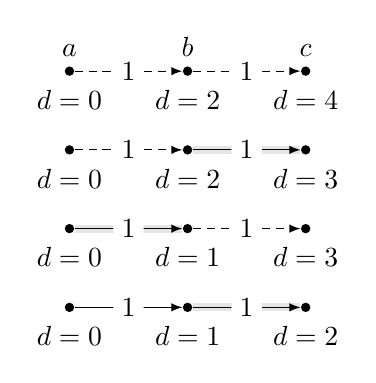
\begin{tikzpicture}
      \tikzset{>=latex} % arrow heads

      \begin{scope}[shift={(0,0)}]
         \node[fill=black,circle,inner sep=1.2pt] (a) at (0,0) {};
         \node[fill=black,circle,inner sep=1.2pt] (b) at (1.5,0) {};
         \node[fill=black,circle,inner sep=1.2pt] (c) at (3.0,0) {};
         \draw[->,densely dashed] (a) -- (b) node[midway,fill=white,circle,inner sep=1pt] {1};
         \draw[->,densely dashed] (b) -- (c) node[midway,fill=white,circle,inner sep=1pt] {1};
         
         \node[above=-0.00cm of a] {$a$};
         \node[above=-0.00cm of b] {$b$};
         \node[above=-0.00cm of c] {$c$};

         \node[below=0.05cm of a] {$d=0$};
         \node[below=0.05cm of b] {$d=2$};
         \node[below=0.05cm of c] {$d=4$};
      \end{scope}

      \begin{scope}[shift={(0,-1)}]
         \node[fill=black,circle,inner sep=1.2pt] (a) at (0,0) {};
         \node[fill=black,circle,inner sep=1.2pt] (b) at (1.5,0) {};
         \node[fill=black,circle,inner sep=1.2pt] (c) at (3.0,0) {};
         \draw[->,densely dashed] (a) -- (b) node[midway,fill=white,circle,inner sep=1pt] {1};
         \draw[line width=0.10cm,black!10] (b) -- (c) node[midway,fill=white,circle,inner sep=1pt] {1};
         \draw[->] (b) -- (c) node[midway,fill=white,circle,inner sep=1pt] {1};

         \node[below=0.05cm of a] {$d=0$};
         \node[below=0.05cm of b] {$d=2$};
         \node[below=0.05cm of c] {$d=3$};
      \end{scope}

      \begin{scope}[shift={(0,-2)}]
         \node[fill=black,circle,inner sep=1.2pt] (a) at (0,0) {};
         \node[fill=black,circle,inner sep=1.2pt] (b) at (1.5,0) {};
         \node[fill=black,circle,inner sep=1.2pt] (c) at (3.0,0) {};
         \draw[line width=0.10cm,black!10] (a) -- (b) node[midway,fill=white,circle,inner sep=1pt] {1};
         \draw[->] (a) -- (b) node[midway,fill=white,circle,inner sep=1pt] {1};
         \draw[->,densely dashed] (b) -- (c) node[midway,fill=white,circle,inner sep=1pt] {1};
         
         \node[below=0.05cm of a] {$d=0$};
         \node[below=0.05cm of b] {$d=1$};
         \node[below=0.05cm of c] {$d=3$};
      \end{scope}

      \begin{scope}[shift={(0,-3)}]
         \node[fill=black,circle,inner sep=1.2pt] (a) at (0,0) {};
         \node[fill=black,circle,inner sep=1.2pt] (b) at (1.5,0) {};
         \node[fill=black,circle,inner sep=1.2pt] (c) at (3.0,0) {};
         \draw[->] (a) -- (b) node[midway,fill=white,circle,inner sep=1pt] {1};
         \draw[line width=0.10cm,black!10] (b) -- (c) node[midway,fill=white,circle,inner sep=1pt] {1};
         \draw[->] (b) -- (c) node[midway,fill=white,circle,inner sep=1pt] {1};
         
         \node[below=0.05cm of a] {$d=0$};
         \node[below=0.05cm of b] {$d=1$};
         \node[below=0.05cm of c] {$d=2$};
      \end{scope}
      
   \end{tikzpicture}
   \caption{Ordering problems.
      Consider the vertices $a \rightarrow b \rightarrow c$,
      with edges $e_{ab}$ and $e_{bc}$ both in tension;
      if $e_{bc}$ is relaxed before $e_{ab}$,
      then $e_{bc}$ will need to be relaxed a second time.}
   \label{fig:ibid:bellman-ford-repetitions}
\end{marginfigure}

We can exploit our intution to order relaxations from start to destination
in the special case where $w \geq 0$
(note that this requirement is stronger than requiring no reachable
negative-length cycles).
We can then show that our approximation $d$
is \emph{sound} for a subset of vertices
as described by Theorem~\ref{thm:ibid-relaxation-sound}.

\begin{marginfigure}
   \centering
   \includegraphics{build/ibid-dijkstra-trust}
   \caption{Tensioned edge trust region
      for $w \geq 0$.
      Contours are of the current estimate $d$.
      Currently tensioned edges are bold and dotted.}
\end{marginfigure}

\begin{theorem}
Consider $d: V \rightarrow \mathbb{R}$
satisfying (\ref{eqn:ibid-relaxation-props-nounder} --
\ref{eqn:ibid-relaxation-props-ds0}),
and let $D$ be the smallest value $d(u)$
among all tensioned edges $e_{uv}$
(or $\infty$ if no such edges exist).
If $w \geq 0$,
any vertex $x$ with $d(x) \leq D$
has $d(x) = d^*(x)$.
\label{thm:ibid-relaxation-sound}
\end{theorem}
As a result,
a given value $D$ creates a region of vertices
with values $d(x) \leq D$ that are known to be
accurate.
This confers two distinct advantages when designing an algorithm:
an efficient relaxation ordering,
and an early termination condition for single-pair problems.

\paragraph{Efficient Relaxation Ordering.}
Therefore,
all tensioned edges $e_{uv}$ with $d(u) = D$
(of which there must be at least one if any edges are tensioned)
can be relaxed immediately,
and will never be retensioned.
This is exactly the order imposed by the OPEN list in Dijkstra's
algorithm \citep{dijkstra1959anote}.

\begin{marginfigure}%
   \centering%
   \includegraphics[width=5cm]{figs/incbi-road-ne/singleshot/example-dijkstra.png}%
   \caption{Dijkstra's algorithm computes the start distance function
      $d^*$ to solve the example shortest path problem.
      Darker vertices have smaller $d$-values.
      The algorithm stops upon reaching the target vertex $t$
      after expanding 1,290,820 vertices.}%
   \label{fig:ibid:example-distance}%
\end{marginfigure}

\paragraph{Early Termination.}
The soundness result shows that once the destination
vertex $t$ satisfies $d(t) \leq D$,
it has the correct start distance.
Since we are only interested in reconstructing a shortest path to $t$,
we are interested in terminating computation of the distance
function as early as possible.

However,
while Theorem~\ref{thm:ibid-relaxation-sound} demonstrates
that $d(t) = d^*(t)$,
it is not by itself insufficient
to demonstrate that such a shortest path to $t$ can be reconstructed.
An illustration of such a problem case is given in
Figure~\ref{fig:ibid:relaxation-completeness-issue}.
This requres the addition of
Theorem~\ref{thm:ibid-relaxation-reconstruct} below.
Notably,
the proof for Theorem~\ref{thm:ibid-relaxation-reconstruct}
relies on (\ref{eqn:ibid-relaxation-props-nottoogood}).

\begin{marginfigure}
   \centering
   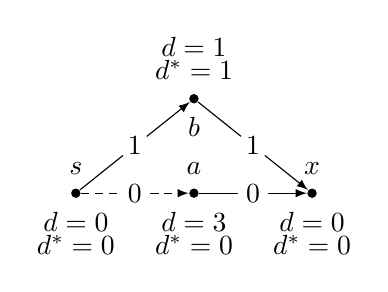
\begin{tikzpicture}
      \tikzset{>=latex} % arrow heads
      \node[fill=black,circle,inner sep=1.2pt] (s) at (0,0) {};
      \node[fill=black,circle,inner sep=1.2pt] (a) at (1.5,0) {};
      \node[fill=black,circle,inner sep=1.2pt] (b) at (1.5,1.2) {};
      \node[fill=black,circle,inner sep=1.2pt] (x) at (3.0,0) {};
      \draw[->,densely dashed] (s) -- (a) node[midway,fill=white,circle,inner sep=1pt] {0};
      \draw[->] (a) -- (x) node[midway,fill=white,circle,inner sep=1pt] {0};
      \draw[->] (s) -- (b) node[midway,fill=white,circle,inner sep=1pt] {1};
      \draw[->] (b) -- (x) node[midway,fill=white,circle,inner sep=1pt] {1};

      \node[above=0.05cm of s] {$s$};
      \node[above=0.05cm of a] {$a$};
      \node[below=0.05cm of b] {$b$};
      \node[above=0.05cm of x] {$x$};

      \node[below=0.05cm of s] {$d=0$};
      \node[below=0.05cm of a] {$d=3$};
      \node[above=0.35cm of b] {$d=1$};
      \node[below=0.05cm of x] {$d=0$};

      \node[below=0.35cm of s] {$d^*=0$};
      \node[below=0.35cm of a] {$d^*=0$};
      \node[above=0.05cm of b] {$d^*=1$};
      \node[below=0.35cm of x] {$d^*=0$};
   \end{tikzpicture}
   \caption{Problem case for pathfinding with distance functions
      in cases where invariant (\ref{eqn:ibid-relaxation-props-nottoogood})
      does not hold.
      Here, $d$ satisfied a and c, with edge $e_{sa}$ tensioned,
      and $d' = 0$.
      While the approximation $d$ is \emph{sound} at $x$
      via Theorem~\ref{thm:ibid-relaxation-sound}
      (i.e. $d(x)$ is correct),
      the path reconstructed from $t$ is not a shortest path.}
   \label{fig:ibid:relaxation-completeness-issue}
\end{marginfigure}

\begin{theorem}
Consider $d: V \rightarrow \mathbb{R}$
satisfying (\ref{eqn:ibid-relaxation-props-nounder} --
\ref{eqn:ibid-relaxation-props-nottoogood}),
and let $D$ be the smallest value $d(u)$
among all tensioned edges $e_{uv}$
(or $\infty$ if no such edges exist).
If $w \geq 0$,
for any vertex $x$ with $d(x) \leq D$,
a path reconstructed backwards from $x$ by iteratively selecting a
predecessor minimizing $d(u) + w(e_{uv})$ until $s$ is reached
is a shortest path from $s$ to $x$ of length $d^*(x)$.
\label{thm:ibid-relaxation-reconstruct}
\end{theorem}

Armed with Theorems~\ref{thm:ibid-relaxation-sound}
and~\ref{thm:ibid-relaxation-reconstruct},
we can terminate edge relaxation early
and reconstruct a shortest path from $s$ to $t$.
This algorithm is listed as ``Dijk''
(Dijkstra's algorithm)
in the results of Figure~\ref{fig:ibid:road-ne-stats}.

\subsection{Bidirectional Search}
\label{sec:ibid:bidirectional}

A prominent technique for minimizing pathfinding computation for
single-pair problems
is bidirectional search
(also called ``doubletree'' search \citep{doran1966doubletree}).
In a bidirectional algorithm,
the distance $d_t$ to the dstination is calculated in a growing region
around the target vertex $t$
concurrently with the conventional start distance $d_s$ around $s$
(Figure~\ref{fig:ibid:example-bidirectional}).
The destination distance function $d_t$,
yielding the distance of a shortest path from each vertex $u$ to $t$,
obeys a complementary definition and local characterization as $d_s$,
with vertex predecessors replaced with successors.
Approaches such as edge relaxation (Section~\ref{subsec:ibid-tension})
can therefore be used to calculate $d_t$ using a region around $t$
within which shortests paths can be reconstructed.

Loosely speaking,
the search can terminate with a shortest path
once the two regions intersect.
The savings relative to a unidirectional search grow with the problem's
branching factor.
For roadmap graphs embedded in an ambient space,
this branching factor can be linear or exponential in the space's
dimension.
\begin{marginfigure}%
   \centering%
   \includegraphics[width=5cm]{figs/incbi-road-ne/singleshot/example-bidijkstra.png}%
   \caption{The bidirectional Dijkatra's algorithm
      computes $d_s$ around the source vertex
      and $d_t$ around the target vertex.
      Darker vertices have smaller $d$-values in their respective
      regions.
      The algorithm terminates after expanding a total of
      1,178,200 vertices using distance to balance expansions.}%
   \label{fig:ibid:example-bidirectional}%
\end{marginfigure}

The first bidirectional algorithm
was proposed by Dantzig \citep{dantzig1963linearprogramming},
and the first precisely described algorithm was presented by
Nicholson \citep{nicholson1966shortest},
%Implementation of a sound and efficient algorithm
%turns on two important questions:
%(a) when and how to terminate with a shortest path,
%and (b) how to balance expansions from the two directions of the
%search.
and the similar Bi-Directional Shortest Path Algorithm (BSPA)
was analyzed by Pohl \citep{pohl1971bidirectional}.
Implementation of a sound and efficient algorithm
turns on when and how to terminate with a shortest path.

\paragraph{A Correct Termination Condition.}
%\label{sec:ibid:bidirectional-termination}
What happens upon an encounter between the forward and reverse searches?
Consider running each search until the first vertex is found
that satisfies Theorem~\ref{thm:ibid-relaxation-sound} in both
directions
(that is, the first vertex $x$ for which
$d_s(x) \leq D_s$ and $d_t(x) \leq D_t$).
While Theorem~\ref{thm:ibid-relaxation-sound} correctly demonstrates
that the values $d_s(x)$ and $d_t(x)$ are correct
(and Theorem~\ref{thm:ibid-relaxation-reconstruct} similarly
demonstrates that a shortest path can be reconstructed from $s$ to $x$
and also from $x$ to $t$),
this is not sufficient to demonstrate that the shortest path
actually passes through $x$.
See Figure~\ref{fig:ibid:bidirectional-termination-issue} for a
counter-example that illustrates this point.

\begin{marginfigure}
   \centering
   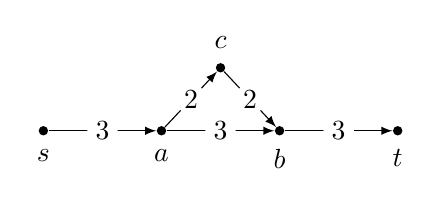
\begin{tikzpicture}
      \tikzset{>=latex} % arrow heads
      \node[fill=black,circle,inner sep=1.2pt] (s) at (0,0) {};
      \node[fill=black,circle,inner sep=1.2pt] (a) at (1.5,0) {};
      \node[fill=black,circle,inner sep=1.2pt] (b) at (3.0,0) {};
      \node[fill=black,circle,inner sep=1.2pt] (t) at (4.5,0) {};
      \node[fill=black,circle,inner sep=1.2pt] (c) at (2.25,0.8) {};
      \draw[->] (s) -- (a) node[midway,fill=white,circle,inner sep=1pt] {3};
      \draw[->] (a) -- (b) node[midway,fill=white,circle,inner sep=1pt] {3};
      \draw[->] (b) -- (t) node[midway,fill=white,circle,inner sep=1pt] {3};
      \draw[->] (a) -- (c) node[midway,fill=white,circle,inner sep=1pt] {2};
      \draw[->] (c) -- (b) node[midway,fill=white,circle,inner sep=1pt] {2};
      \node[below=0.05cm of s] {$s$};
      \node[below=0.05cm of a] {$a$};
      \node[below=0.05cm of b] {$b$};
      \node[below=0.05cm of t] {$t$};
      \node[above=0.05cm of c] {$c$};
   \end{tikzpicture}
   \caption{Simple illustration of a problem case for terminating
      a bidirectional search.
      With a balanced distance criterion,
      $c$ will be the first vertex expanded in both directions,
      but it does not lie on the shortest path.}
   \label{fig:ibid:bidirectional-termination-issue}
\end{marginfigure}

Importantly, is nececessary to consider the \emph{edges} connecting
the two distance function approximations.
A correct termination condition is surprisingly subtle,%
\marginnote{There were early incorrect attempts at a sound
termination condition
\citep{berge1965programminggamestransportation}.}
with several correct variations proposed
\citep{nicholson1966shortest, dreyfus1969appraisalsp,
pohl1969bidirectional, goldberg2005spexternalmemory}.
What is necessary is a bidirectional equivalent to the 
completeness-based termination condition
from Theorem~\ref{thm:ibid-relaxation-reconstruct}.

Suppose $d_s$ and $d_t$ are approximations to $d^*_s$ and $d_t^*$,
respectively,
with each satisfying (\ref{eqn:ibid-relaxation-props}).
Let $D_s$ be the minimum $u$-value among all tensioned edges in $d_s$
(and likewise for $d_t$).
Then we can establish the following proof of a correct termination
condition:

\marginnote{This treatment of the bidirectional termination condition
is presented differently than in most related work because it will
help us formulate an incremental version
in Section~\ref{sef:ibid:ibid}.}

\begin{theorem}
Define $E_{\ms{conn}}$ as the set of all edges $e_{uv}$ such that
$d_s(u) \leq D_s$ and $d_t(v) \leq D_t$,
and define $\ell_e$ s.t. $\ell_e(e_{uv}) = d_s(u) + w(e_{uv}) + d_t(v)$.
If $w \geq 0$,
$s \neq t$,
$E_{\ms{conn}}$ is non-empty,
and $e^*_{uv}$ minimizes $\ell_e$
among $E_{\ms{conn}}$ with $\ell_e(e^*_{uv}) \leq D_s + D_t$,
then $\ell_e(e^*_{uv})$ is the length of the shortest path,
and $e^*_{uv}$ lies on one such path.
\label{thm:ibid-bidir-sound}
\end{theorem}

\paragraph{Designing an Efficient Bidirectional Algorithm.}
In the case where the approximations $d_s$ and $d_t$ are improved
via edge relaxation,
since $w \geq 0$,
by Theorem~\ref{thm:ibid-relaxation-sound}
once an edge $e_{uv}$ becomes included in
$E_{\ms{conn}}$,
its length value $\ell_e(e_{uv})$ will not change.
Therefore,
it is sufficient for a relaxation algorithm to consider only edges
newly added to $E_{\ms{conn}}$ at each iteration,
and keep track of the best edge $e^*_{uv}$
with its value $\ell_e(e^*_{uv})$ found so far.
Note also that Theorem~\ref{thm:ibid-relaxation-reconstruct}
allows a shortest path to be constructed from $e^*_{uv}$
buy walking backwards from $u$ to $s$,
and forwards from $v$ to $t$.

This algorithm is listed as ``BiDijk''
(bidirectional Dijkstra's algorithm)
in the results of Figure~\ref{fig:ibid:road-ne-stats}.

%\subsection{Balancing Directions}
%The general bidirectional algorithm leaves open the strategy
%used to balance the progression of the two search directions.
%Options based on alternating \citep{dantzig1963linearprogramming},
%or selecting the direction with the smaller {\sc Open} distance
%\citep{nicholson1966shortest}
%or {\sc Open} (and finite) set cardinality
%\citep{pohl1969bidirectional}
%have been proposed.
%Note that while some literature asserts that
%these can be interleaved arbitrarily,
%termination of the algorithm requires that each direction
%be expanded at least once.
%Our example problems use the balanced distance criterion.

\subsection{Incremental Search for Dynamic Problems}
\label{sec:ibid:incremental}

The shortest path on a graph is of course intimately tied to
the edge weight function $w$.
If the weight function changes from $w^{(1)}$ to $w^{(2)}$,
a shortest path $p^{(1)}$ w.r.t. $w^{(1)}$
will generally no longer be a shortest path w.r.t. $w^{(2)}$,
even if changes are small and localized.
For example,
if the weight of edge on $p^{(1)}$ increases,
or if the weight of some edge not on $p$ decreases,
then some other path $p^{(2)}$ may become shorter than $p^{(1)}$.
The \emph{dynamic shortest-path problem}
considers finding a shortest path
for each of a sequence of input edge weight functions.
Figure~\ref{fig:ibid:example-incremental}
shows an incremental algorithm finding a shortest path quickly
for a subsequent planning episode.

\begin{marginfigure}%
   \centering%
   \subfloat[Initial episode]{%
      \centering%
      \includegraphics[width=5cm]{figs/incbi-road-ne/singleshot/example-incuni-0.png}%
   }
   
   \subfloat[Subsequent episode]{%
      \centering%
      \includegraphics[width=5cm]{figs/incbi-road-ne/singleshot/example-incuni-1.png}%
   }%
   \caption{Initial episode: 1,287,897 expansions.
      Subsequent episode: 391,122 expansions.}%
   \label{fig:ibid:example-incremental}%
\end{marginfigure}

We concern ourselves with the \emph{fully dynamic} case,
in which arbitrary edge weight changes are allowed.
As mentioned in Section~\ref{subsec:ibid-probdef},
for our pathfinding problems,
we treat edges with infinite weight equivalently with non-existant
edges.
Therefore,
deleting or inserting an edge can be represented by
setting its edge weight to or from infinity, respectively.
We include here a brief review of the approach underlying common
algorithms for the dynamic pathfinding problem.

The dynamic problem has been studied in the literature.
Eary results demonstrated properties of optimal spanning trees
under certain types of update operations
\citep{spirapan1975updatingsp}.
Early algorithms considered restricted problem such as
the insert-only problem
with constant edge weights \citep{linchang1991dynamicsp},
or restricted settings such as planar graphs
\citep{klein1998planardynamicshort}.
More general algorithms followed
\citep{ramalingam1996dynamicswsffp,
   frigioni1996dynamicsinglesource,
   frigioni2000dynamicsp}.
\marginnote{We defer for now discussing the problem of integrating
heuristic functions with incremental search;
see Section~\ref{subsec:ibid:heuristic-incremental}
for that discussion.}
A review of more general dynamic problems on graphs is available
in \citep{eppstein1999dynamic},
including for the more general all-pairs problem
\citep{demetrescu2010dynamic}.

\paragraph{Problem Definition.}
Consider a directed graph $G = (V,E)$ as described in
Section~\ref{subsec:ibid-probdef}.
Consider a sequence of pathfinding episodes
with different edge weight functions $w^{(1)}, w^{(2)}, \dots$
with $w^{(i)} : E \rightarrow \mathbb{R}$.
The dynamic single-pair shortest-path (SPSP) problem
entails finding shortest paths $p^{(1)}, p^{(2)}, \dots$
between fixed start and destination vertices $s,t \in V$
for each episode.

\paragraph{Approches to the Dynamic Problem.}
The simplest class of solutions to the dynamic SPSP problem
entails running a conventional SPSP algorithm to compute a solution
path for episode in turn.
Consider, for example, applying the edge relaxation approach
from Section~\ref{subsec:ibid-tension}
to compute the start distance function $d_s^{(i)}$ from scratch
for each episode's edge weight function $w^{(i)}$.

Investigating this approach more closely reveals an opportunity for
a more efficient algorithm.
If the changes in the weight function between each episode affect
only a subset of the edges,
then it is often the case that the value of the distance function
computed does not change for a large fraction of the vertices in the
graph.
In the face of a change in weight function
$w^{(i)} \rightarrow w^{(i+1)}$,
it is the objective of an \emph{incremental} approach
to adapt a previously computed estimate $d_s^{(i)}$
to a new one $d_s^{(i+1)}$ with a minimal amount of additional
computation.

\paragraph{Inapplicability of the Tensioned Estimates Approach.}
The tensioned estimates approach of Section~\ref{subsec:ibid-tension}
made use of two clever devices to allow its approximation $d$ to be
iteratively improved to the true distance function $d^*$.
First, it relied on a global invariant
(\ref{eqn:ibid-relaxation-props-nounder})
to ensure that the approximation was never under-consistent.
Second, it relied on a decomposition of the local characterization
(\ref{eqn:distance-function-char})
into two inequalities
(\ref{eqn:ibid-relaxation-props-nottoogood})
and (\ref{eqn:ibid-relaxation-props-tens}),
the former treated as a second invariant,
and the latter represented not as a constraint but as a labeling
of tensioned edges to be iteratively relaxed.

Unfortunately,
the incremental setting precludes this approach.
Consider a new episode in which the estimate $d^{(i+1)}$
is initialized with the preceeding estimate $d^{(i)}$.
Since the weight function $w^{(i+1)}$ has changed,
there is no guarantee that either of the invariants
(\ref{eqn:ibid-relaxation-props-nounder})
or (\ref{eqn:ibid-relaxation-props-nottoogood}) still hold.
In particular,
if edge weights increase,
it is common for one or both invariants to be violated,
and we can no longer rely on Theorems~\ref{thm:ibid-relaxation-sound}
or~\ref{thm:ibid-relaxation-reconstruct} to generate sound
shortest paths.

\paragraph{A New Approach.}
The key idea underlying the incremental approach,
and the DynamicSWSF-FP \citep{ramalingam1996dynamicswsffp} algorithm,
is to restate the local characterization (\ref{eqn:distance-function-char})
in a different way.
In particular:
\begin{subequations}%
   \begin{eqnarray}
      & r(v) = 
         \left\{ \begin{array}{cl}
            0 & \mbox{if } v = s \\
            \displaystyle\min_{u \in \mbox{\scriptsize Pred}(v)} d(u) + w(e_{uv}) & \mbox{otherwise} \\
         \end{array} \right.
         & \label{eqn:ibid-inc-props-rvalue} \\
      & d(v) = r(v)
         & \label{eqn:ibid-inc-props-consistent}
   \end{eqnarray}%
   \label{eqn:ibid-inc-props}%
\end{subequations}%
(Here, $r(v)$ represents the ``right-hand side'' of
the local characterization).
It is easy to see how (\ref{eqn:ibid-inc-props}) taken together
directly implies (\ref{eqn:distance-function-char}).
The motivation behind this decomposition is that the former
(\ref{eqn:ibid-inc-props-rvalue}) can be held as an invariant,
while the latter (\ref{eqn:ibid-inc-props-consistent})
can be established iteratively.
Prior work adopts the following labeling for each vertex $v$:
if $d(v) = r(v)$, the vertex is \emph{consistent},
whereas inconsistent vertices are either
\emph{under-consistent} if $d(v) < r(v)$
or \emph{over-consistent} if $d(v) > r(v)$.

Importantly,
the inapplicability of the global invariant
(\ref{eqn:ibid-relaxation-props-nounder}) between episodes
has implications on the class of weight functions that can be solved
by the incremental approach.
In particular,
when applied to weight functions with cycles of zero length
(for which $d^*$ is well-defined),
there is no guarantee that a distance function $d$
which satisfies (\ref{eqn:ibid-inc-props-consistent})
matches $d^*$.
We therefore restrict the class of weight functions considered
to those with only positive length cycles.

\cdnote{TODO: show that the algorithm terminates as long as there
are no cycles with non-positive length.
Lyaponov function argument?}

\paragraph{Approximation Soundness.}
In Section~\ref{subsec:ibid-tension},
we showed that in cases with $w \geq 0$,
the minimal value $k$ defines a trust region that can be used both
to order edge relaxations as well as inform a termination condition
after which a correct path can be reconstructed.
We can develop a similar argument about the soundness of an
approximation in the dynamic case.
In particular,
given an arbitrary estimate $d$
(and the corresponding function $r$ as defined by
(\ref{eqn:ibid-inc-props-rvalue}),
this argument makes use of a third function $k$ defined as:
\begin{equation}
   k(v) = \min\left[ d(v), r(v) \right].
   \label{eqn:ibid:incremental-key}
\end{equation}
%If we define $V_{\ms{incons}}$ as the set of inconsistent vertices
%(that is, with $d(v) \neq r(v)$,
%then we define the value $k_{\ms{min}}$ as:
%\begin{equation}
%   k_{\ms{min}} = \displaystyle\min_{v \in V_{\ms{incons}}} \left[ k(v) \right]
%\end{equation}
We can then establish the following central soundness result
for incremental search:

\begin{theorem}
Consider $d: V \rightarrow \mathbb{R}$,
with $r$ satisfying (\ref{eqn:ibid-inc-props-rvalue}),
and let $K$ be the smallest value $k(v)$
among all inconsistent vertices
(or $\infty$ if no such vertices exist).
If $w > 0$,
any consistent vertex $x$ with $d(x) \leq K$
has $d(x) = d^*(x)$.
Further,
walking backwards from $x$ choosing predecessors that minimize
$d(u) + w(e_{uv})$ terminates at $s$ with a shortest path
of length $d^*(x)$.
\label{thm:ibid-dynamicswsffp-sound}
\end{theorem}

This theorem enables the same two efficiency advantages as in
the relaxation approach, in the case where $w > 0$.
It provides that a vertex rendered consistent during an iteration
(by setting $d(x) \leftarrow r(x)$) with $d(x) \leq K$
has the correct value and will never be revisited.
It also enables an algorithm to terminate early
once the destination vertex $t$ becomes consistent,
as exploited by the Lifelong Planning A* algorithm
\citep{koenig2004lpastar}.

\subsection{Algorithm Design}

\cdnote{I still need to write this part!
Talk about queues!}

This algorithm is listed as ``DynSWSF''
(Dynamic SWSF-FP)
in the results of Figure~\ref{fig:ibid:road-ne-stats}.


% I don't need this anymore, subsumed in soundness result!
%\paragraph{Approximation Completeness.}
%
%For bidirectional search,
%it's also necessary to be able to prove that you have found
%all vertices within a certain distance of the start.
%Basically, this is a completeness proof --
%if a distance exists below a certain value,
%we will have found it.
%This is completeness of the approximation,
%not of an algorithm per se.
%
%\begin{theorem}
%Any vertex $x$ with $d^*(x) < k_{\ms{min}}$
%has $d(x) = d^*(x)$.
%\label{thm:ibid-dynamicswsffp-complete}
%\end{theorem}
%
%\begin{proof}[Proof of Theorem~\ref{thm:ibid-dynamicswsffp-complete}]
%We show that $d(x)$ can be both
%no less than $d^*(x)$
%(Lemma~\ref{lemma:ibid-dynamicswsffp-complete-geq})
%and no greater than $d^*(x)$
%(Lemma~\ref{lemma:ibid-dynamicswsffp-complete-leq}).
%\end{proof}
%
%\begin{lemma}
%Any vertex $x$ with $d^*(x) < k_{\ms{min}}$
%has $d(x) \geq d^*(x)$.
%\label{lemma:ibid-dynamicswsffp-complete-geq}
%\end{lemma}
%
%\begin{proof}[Proof of Lemma~\ref{lemma:ibid-dynamicswsffp-complete-geq}]
%We show this by contradiction.
%Suppose there exists a vertex $x$ with $d^*(x) < k_{\ms{min}}$
%for which $d(x) < d^*(x)$.
%Then $d(x) < k_{\ms{min}}$,
%so $x$ must be consistent.
%By Lemma~\ref{lemma:ibid-dynamicswsffp-sound-geq},
%we must have $d(x) \geq d^*(x)$.
%This contradicts our supposition.
%\end{proof}
%
%\begin{lemma}
%Any vertex $x$ with $d^*(x) < k_{\ms{min}}$
%has $d(x) \leq d^*(x)$.
%\label{lemma:ibid-dynamicswsffp-complete-leq}
%\end{lemma}
%
%\begin{proof}[Proof of Lemma~\ref{lemma:ibid-dynamicswsffp-complete-leq}]
%This proof proceeds in a similar way to that for
%Lemma~\ref{lemma:ibid-dynamicswsffp-sound-leq}.
%Construct a true shortest path from $s$ to $x$,
%with $d^*$-values increasing monotonically from
%$d^*(s) = 0$ to $d^*(x)$.
%Consider each edge $e_{uv}$ in turn as follows.
%Assume that $u$ is consistent,
%with $d(u) \leq d^*(u)$.
%Note that this is true for the first edge with $u = s$,
%since with $0 \leq d^*(x)$,
%we have $0 < k_{\ms{min}}$,
%so that $s$ must is consistent with $r(s) = d(s) = d^*(s) = 0$.
%Since $e_{uv}$ lies on a true shortest path,
%we must have $d^*(u) + w(e_{uv}) = d^*(v)$,
%and for all edges $d(u) + w(e_{uv}) \geq r(v)$.
%Together, this implies that
%$d^*(u) - d(u) \leq d^*(v) - r(v)$.
%Our assumption that $d(u) \leq d^*(u)$
%therefore implies that $r(v) \leq d^*(v)$.
%Since $d^*(v) \leq d^*(x)$ and $d^*(x) < k_{\ms{min}}$,
%we know that $v$ is consistent,
%so we conclude that $d(v) \leq d^*(v)$,
%and we can proceed to the next edge on the path.
%We end with $v = x$,
%so that $d(x) \leq d^*(x)$.
%\end{proof}

\section{Incremental Bidirectional Search}
\label{sef:ibid:ibid}

The principal motivation behind
the Incremental Bidirectional (IBiD) search algorithm
is to leverage the early termination efficiency of a bidirectional search
with the efficiency of an incremental search for dynamic
single-pair shortest path problems.
An example of IBiD is shown in
Figure~\ref{fig:ibid:example-incremental-bidirectional}.
\begin{marginfigure}%
   \centering%
   \subfloat[Initial search]{%
      \centering%
      \includegraphics[width=5cm]{figs/incbi-road-ne/singleshot/example-incbi-0.png}%
   }
   
   \subfloat[Replan search]{%
      \centering%
      \includegraphics[width=5cm]{figs/incbi-road-ne/singleshot/example-incbi-1.png}%
   }%
   \caption{Initial search: 1,181,616 expansions.
      Replan: 262,422 expansions.}%
   \label{fig:ibid:example-incremental-bidirectional}%
\end{marginfigure}

\subsection{Bidirectional Termination with Incremental Distance Functions}

Consider a graph endowed with two distance functions,
a start distance approximation $d_s$,
and a destination distance approximation $d_t$.
Since this is an incremental setting,
we can make use of the formulation
of Theorem~\ref{thm:ibid-dynamicswsffp-sound}
from Section~\ref{sec:ibid:incremental}
to establish the correctness of these approximations
for certain vertices.

It is essential that the bidirectional termination condition from
Theorem~\ref{thm:ibid-bidir-sound} be adapted to
handle these incrementally maintained distance functions.
The central theorem that enables the IBiD algorithm is:

\begin{theorem}
Consider a graph with $w > 0$ and with $s \neq t$.
Consider a start distance approximation $d_s: V \rightarrow \mathbb{R}$,
with $r_s$ satisfying (\ref{eqn:ibid-inc-props-rvalue}),
and let $K_s$ be the smallest value $k_s(v)$
among all inconsistent vertices,
or $\infty$ if no such vertices exist;
likewise, consider the same for a destination distance approximation
$d_t$ and its accompanying $r_t$ and $K_t$.

Define $E_{\ms{conn}}$ as the set of all edges $e_{uv}$ such that
$u$ is $s$-consistent with $d_s(u) \leq K_s$
and $v$ is $t$-consistent with $d_t(v) \leq K_t$,
and define $\ell_e$ s.t. $\ell_e(e_{uv}) = d_s(u) + w(e_{uv}) + d_t(v)$.
If $E_{\ms{conn}}$ is non-empty,
and $e^*_{uv}$ minimizes $\ell_e$
among $E_{\ms{conn}}$ with $\ell_e(e^*_{uv}) \leq K_s + K_t$,
then $\ell_e(e^*_{uv})$ is the length of the shortest path,
and $e^*_{uv}$ lies on one such path.
\label{thm:ibid-sound}
\end{theorem}

Note that the first half of the conditions
from Theorem~\ref{thm:ibid-sound}
is drawn from the soundness conditions for incremental search
from Theoem~\ref{thm:ibid-dynamicswsffp-sound},
while the second half resembles the bidirectional termination
conditions from Theorem~\ref{thm:ibid-bidir-sound}.

\subsection{Algorithm Design}

\paragraph{Simultaneous Incremental Searches.}
The IBiD algorithm runs two independent conventional
DynamicSWSF-FP \citep{ramalingam1996dynamicswsffp}
searches simultaneously,
one from the start vertex $s$
and one from the destination vertex $t$,
with each maintaining a separate priority queue of
inconsistent vertices $Q_s$ and $Q_t$ respectively
(Algorithm~\ref{alg:ibid-two-dynamicswsffps}).

As with a convential bidirectional search,
the two sides can be alternated arbitrarily,
except that the each queue must be processed once upon initialization
so that $d_s(s) = 0$ and $d_t(t) = 0$.

{\floatevery{algorithm}{\setlength\hsize{16.85cm}}
\begin{algorithm}[t]
   \caption{As a bidirectional algorithm,
      IBiD conducts two independent DynamicSWSF-FP searches,
      one computing distance from the start vertex $s$,
      and the other computing distance to the destination vertex $t$.}
   \label{alg:ibid-two-dynamicswsffps}
   \begin{minipage}[t]{8.2cm}
      \begin{algorithmic}[1]
         \Procedure {InitializeSource} {\,\!}
            \ForAll {$v \in V$}
               \State $d_s(v) \gets \infty; \;\; r_s(v) \gets \infty$
            \EndFor
            \State $r_s(s) \gets 0$
            \State $Q_s \gets \{ s \}$
               \Comment $\mbox{ key for } v: \min\big(r_s(v),d_s(v)\big)$
            \State $\mbox{\sc ProcessSourceQueue}()$
         \EndProcedure
         \Procedure {UpdateSourceDistance} {$v$}
            \If {$v \neq s$}
               \State $r_s(v) \gets \displaystyle\min_{u \in \mbox{\scriptsize Pred}(v)}
                  \big( d_s(u) + w(u,v) \big)$
            \EndIf
            \State Ensure $v \in Q_s$ iff $d_s(v) \neq r_s(v)$
         \EndProcedure
         \Procedure {ProcessSourceQueue} {\,\!}
            \State $u \gets Q_s.\mbox{Pop}()$
            \If {$r_s(u) < d_s(u)$}
                  \Comment over-consistent
               \State $d_s(u) \gets r_s(u)$
               \ForAll {$v \in \mbox{Succ}(u)$}
                  \State $\mbox{\sc UpdateSourceDistance}(v)$
               \EndFor
            \Else
                  \Comment under-consistent
               \State $d_s(u) \gets \infty$
               \ForAll {$v \in \mbox{Succ}(u) \cup u$}
                  \State $\mbox{\sc UpdateSourceDistance}(v)$
               \EndFor
            \EndIf
         \EndProcedure
         \algstore{ibid-two-dynamicswsffps}
      \end{algorithmic}
   \end{minipage}
   \quad
   \begin{minipage}[t]{8.2cm}
      \begin{algorithmic}[1]
         \algrestore{ibid-two-dynamicswsffps}
         \Procedure {InitializeTarget} {\,\!}
            \ForAll {$v \in V$}
               \State $d_t(v) \gets \infty; \;\; r_t(v) \gets \infty$
            \EndFor
            \State $r_t(t) \gets 0$
            \State $Q_t \gets \{ t \}$
               \Comment $\mbox{ key for } v: \min\big(r_t(v),d_t(v)\big)$
            \State $\mbox{\sc ProcessTargetQueue}()$
         \EndProcedure
         \Procedure {UpdateTargetDistance} {$u$}
            \If {$u \neq t$}
               \State $r_t(u) \gets \displaystyle\min_{v \in \mbox{\scriptsize Succ}(u)}
                  \big( w(u,v) + d_t(v) \big)$
            \EndIf
            \State Ensure $u \in Q_t$ iff $d_t(u) \neq r_t(u)$
         \EndProcedure
         \Procedure {ProcessTargetQueue} {\,\!}
            \State $v \gets Q_t.\mbox{Pop}()$
            \If {$r_t(v) < d_t(v)$}
                  \Comment over-consistent
               \State $d_t(v) \gets r_t(v)$
               \ForAll {$u \in \mbox{Pred}(v)$}
                  \State $\mbox{\sc UpdateTargetDistance}(u)$
               \EndFor
            \Else
                  \Comment under-consistent
               \State $d_t(v) \gets \infty$
               \ForAll {$u \in \mbox{Pred}(v) \cup v$}
                  \State $\mbox{\sc UpdateTargetDistance}(u)$
               \EndFor
            \EndIf
         \EndProcedure
      \end{algorithmic}
   \end{minipage}
\end{algorithm}
} % floatevery width adjustment

\paragraph{Remembering Connections.}
Theorem~\ref{thm:ibid-sound} has ramifications when designing
an algorithm.
In the case of bidirectional search
described in Section~\ref{sec:ibid:bidirectional},
the algorithm could take a shortcut since $D$-values always decreased,
so it was not necessary to remember older edges when better
ones were found.
In the incremental case,
where the start and destination distance functions $d_s$ and $d_t$
may both increase and decrease between episodes,
it is no longer sufficient to remember only the best connection
found so far.

We capture the central idea from Theorem~\ref{thm:ibid-sound}
in Algorithm~\ref{alg:ibid}.
This algorithm is listed as ``IBiD''
in the results of Figure~\ref{fig:ibid:road-ne-stats}.

\begin{algorithm}[t]
   \caption{IBiD Outline}
   \label{alg:ibid}
   \begin{algorithmic}[1]
      \Procedure {Main} {\,}
         \State $\mbox{\sc InitializeSource}(); \; \mbox{\sc InitializeTarget}()$
         \State $Q_c \gets \emptyset$
            \Comment $\mbox{ key for } (u,v): d_s(u) + w(u,v) + d_t(v)$
         \Loop
            \While {not $\mbox{\sc TerminationCondition}()$}
               \If {$Q_s.\mbox{TopKey} < Q_t.\mbox{TopKey}$}
                     \Comment prioritize arbitrarily
                  \State $\mbox{\sc ProcessSourceQueue}(u)$
               \Else
                  \State $\mbox{\sc ProcessTargetQueue}(u)$
               \EndIf
               \State Ensure $(u,v) \in Q_c$ iff
                  $u \neq Q_s$, $v \neq Q_t$, key $\neq \infty$
            \EndWhile
            \State $(u_c,v_c) \gets Q_c.\mbox{Top}$
            \State $\pi \gets
               ( \mbox{walk } d_s \mbox{ from } u_c \mbox{ to } s )
               \cup
               ( \mbox{walk } d_t \mbox{ from } v_c \mbox{ to } t )$
            \State wait for edges $(u,v) \in E_{\ms{delta}}$ with changed weights $w(u,v)$
            \State $\mbox{\sc NotifyWeightChanges}(E_{\ms{delta}})$
         \EndLoop
      \EndProcedure
      \Function {TerminationCondition} {\,}
         \State $(u_c,v_c) \gets Q_c.\mbox{TopKey}$
            \Comment return False if $Q_c$ empty
         \If {$Q_s.\mbox{TopKey} + Q_t.\mbox{TopKey} < d_s(u_c) + w(u_c,v_c) + d_t(v_c)$}
            \State \Return False
         \EndIf
         \If {$Q_s.\mbox{TopKey} < d_s(u_c)$
               \mbox{\bf or} $Q_t.\mbox{TopKey} < d_t(v_c)$}
            \State \Return False
         \EndIf
         \State \Return True
      \EndFunction
      \Procedure {NotifyWeightChanges} {$E_{\ms{delta}}$}
         \ForAll {$(u,v) \in E_{\ms{delta}}$}
            \State $\mbox{\sc UpdateSourceDistance}(v)$
            \State $\mbox{\sc UpdateTargetDistance}(u)$
         \EndFor
         \State Ensure $(u,v) \in Q_c$ iff
            $u \neq Q_s$, $v \neq Q_t$, key $\neq \infty$
      \EndProcedure
   \end{algorithmic}
\end{algorithm}


\section{Heuristic Search}
\label{sec:ibid:heuristic}

When examining how to assemble a heuristic-informed algorithm
that integrates bidirectional with incremental methods,
it's instructive to examine how these efforts have been addressed
in the past.

\paragraph{Review of Heuristic Methods.}
Heuristic methods such as the Graph Traverser
\citep{doran1966graphtraverser} were originally
applied to pathfinding problems in order to find non-optimal
solutions more economically.
These unidirectional methods proceed similarly to Dijkstra's algorithm,
but instead of prioritizing {\sc Open} vertices
based on their source distance $d_s$,
they use a target-directed heuristic function $h_t$.
Hart, Nilsson, and Raphael \citep{hart1968astar} established that
these approaches can be combined ($d_s + h_t$) to yield
an admissible algorithm (A*) for the shortest-path problem,
as long as $h_t$ meets certain conditions.
See Figure~\ref{fig:ibid:example-astar}.
We show the results of unidirectional heuristic search as ``A*''
in the results of Figure~\ref{fig:ibid:road-ne-stats}.

\begin{marginfigure}%
   \centering%
   \includegraphics[width=5cm]{figs/incbi-road-ne/singleshot/example-astar.png}%
   \caption{A* search.
      532,880 expansions.}%
   \label{fig:ibid:example-astar}%
\end{marginfigure}

\subsection{Heuristic Methods in Bidirectional Search.}
\label{subsec:ibid:heuristic-bidirectional}

Attempts to provide a bidirectional algorithm which incorporates
heuristic estimates generally take one of three approaches,
which we survey here.

First,
``front-to-back'' methods
such as Pohl's Bidirectional Heuristic Path Algorithm (BHPA)
\citep{pohl1971bidirectional}
conduct two conventional heuristic-informed searches
(i.e. the start search directed to the goal vertex,
and vice versa).
This approach suffers from the problem that the two sets of
\textsc{Closed} vertices must overlap substantially
before the search can be terminated,
and therefore the benefit of the bidirectional search
is not fully realized.
\cdnote{Pohl cites Berge? Missile analogy.}

Second,
``front-to-front'' methods exploit a consistent pairwise
heuristic function $h(u,v)$ evaluated over every pair of vertices
on each search's \textsc{Open} list,
and the vertices representing the shortest potential path are
expanded.
Early approaches with inflated heuristics
\citep{doran1966doubletree} did not yield promising results.
The later Bidirectional Heuristic Front-to-Front Algorithm
(BHFFA) \citep{champeaux1983biheuragain} does show an improved
number of vertex expansions.
\marginnote{An earlier version of BHFFA \citep{champeauxsint1977bhffa}
was shown to be incorrect due in large part to the difficulty
establishing a correct bidirectional termination condition.}
While this approach does not suffer from the region overlap problem
inherent in front-to-back methods,
it instead incurrs the very high cost of computing full pairwise
heuristics, and updating all vertices on \textsc{Open}
after each vertex expansion.

The third approach
derives from an alternative interpretation of heuristic search
algorithms first proposed by Ikeda et. al.
\citep{ikeda1994betterroutes}.
Under this interpretation,
a heuristic-informed A* search is equivalent to an uninformed
Dijkstra's search under a particular transformation
of the edge weights using the heuristic function
as a vertex potential function.
Therefore,
because front-to-back methods use different heuristics for the
forward and reverse searches,
they are effectively searching graphs with different weight functions.
The proposed solution is to arrive at a single consistent potential
function,
which allows the transformed pathfinding problem to be solved using
the uninformed bidirectional algorithm described
in Section~\ref{sec:ibid:bidirectional}.

\paragraph{Potential-Adjusted Weight Functions.}
Consider an arbitrary vertex potential function
$b : V \rightarrow \mathbb{R}$,
and consider the following transformation of a weight
function $w$ into transformed weight function $w_b$:
\begin{equation}
   w_b(e_{uv}) = w(e_{uv}) - \left[ b(u) - b(v) \right].
   \label{eqn:ibid:potential-transformation}
\end{equation}
The effect of this transformation on the lengths of paths over $G$
bears investigation.
Consider a path $p_{xy}$ from $x$ to $y$ which has length $\ell$ w.r.t. $w$.
What is its weight $\ell_b$ w.r.t. $w_b$?
A simple summation reveals that
\begin{equation}
   \ell_b(p_{xy}) = \ell(p_{xy}) - \left[ b(x) - b(y) \right].
   \label{eqn:ibid:potential-path-lengths}
\end{equation}
That is, the difference between the initial and transformed lengths
of the path from $x$ to $y$ is independent of the path itself
(its consituent vertices and edges),
and only a function of the endpoint vertices.
In particular,
this implies that a shortest path from $x$ to $y$ w.r.t. $w_b$
remains a shortest path w.r.t. $w$.
Therefore, any admissible shortest path algorithm can be used to
solve w.r.t. $w_b$.
Note that the transformation does not change the length of any
cycles in $G$.
Note also that as a consequence of
(\ref{eqn:ibid:potential-path-lengths}),
the original and transformed start distance functions are related by
\begin{equation}
   d^*_b(v) = d^*(v) - \left[ b(s) - b(v) \right].
\end{equation}

\paragraph{Benefit of Potential Adjustment.}
If the ordering of solution paths does not change under the
potential function transformation,
what benefit would be obtained by conducting the search
on the transformed weight function?
Indeed,
computing the full distance function $d_s$ over $w_b$,
e.g. by edge relaxation,
appears just as expensive.

The key insight is that under an appropriately chosen potential function,
many shortest path algorithms are able to terminate more quickly.
To see why,
consider the potential function $b$ coinciding with the goal heuristic
function $h_g$ used in A*.
By (\ref{eqn:ibid:potential-transformation}),
the weight $w_b$ of a directed edge $e_{uv}$ which makes
progress towards the goal (so that $b(v) < b(u)$)
will have its transformed weight be reduced,
whereas an edge in the incorrect direction will have its transformed
weight increase.
The transformed quantity $w_b$
from (\ref{eqn:ibid:potential-transformation})
can be considered the \emph{excess weight} of each edge,
relative to the expected weight given the progress measured by the
heuristic function
(this quantity has also been called the ``waste'' of the edge
\citep{pohl1969bidirectional}).
A pathfinding algorithm therefore searches only in the excess weight
space,
and is therefore biased to explore paths which make progress towards
the goal vertex.
In effect,
while the transformation does not affect the relative ordering of
paths,
it does shift the weight between edges on paths to accentuate poor
choices to allow for early termination.

\paragraph{Requirements on the Potential Function.}
The argument that ordering of paths (and therefore shortest path(s))
is invariant to the transformation is true for any arbitrary
potential function.
However,
in order to be useful,
we must be able to solve the transformed problem efficiently
(i.e. with early termination).
As we saw for edge relaxation in Section~\ref{subsec:ibid-tension},
our soundness result from Theorem~\ref{thm:ibid-relaxation-reconstruct}
requires that the edge weight function be nonnegative.
This induces the requirement that
the vertex potential $b$ to be \emph{consistent}
(also known as \emph{dual feasible}), i.e.
\begin{equation}
   b(u) + w(e_{uv}) \geq b(v) \quad\forall e_{uv} \in E.
   \label{eqn:ibid:potential-consistent}
\end{equation}
If (\ref{eqn:ibid:potential-consistent}) holds,
then the efficient ordering and early termination
for edge relaxation (i.e. Dijkstra's algorithm)
can be applied to the transformed problem $w_b$,
and the returned path is also a shortest path w.r.t. $w$. 

\paragraph{Potential Functions for Bidirectional Search.}
Treating heuristic search as such a potential function transformation
allows Ikeda et. al. \citep{ikeda1994betterroutes} to apply
the same idea to bidirectional search.
In particular,
if one commits to a single potential function $b$,
then the conventional bidirectional algorithm
(Section~\ref{sec:ibid:bidirectional})
can be applied directly.
The question is,
what potential function should we use?

A bidirectional search customarily has available
two heuristic functions,
one $h_t(v)$ that approximates the length of paths
from $v$ to the destination vertex $t$,
and one $h_s(v)$ that approximates the length of paths
from the start vertex to $v$.
The most commonly used potential function
\citep{ikeda1994betterroutes, goldberg2005spexternalmemory}
is simply the average of the two:
\begin{equation}
   b(v) = \frac{h_t(v) - h_s(v)}{2}.
\end{equation}
Note that the start heuristic value is negated;
when the start heuristic is used during the reverse search,
it is applied to predecessor vertices.
Figure~\ref{fig:ibid:example-heurbidijkstra} shows this averaged
potential function for the example road network problem.
This algorithm is listed as ``W-BiDijk''
(weighted bidirectional Dijkstra's)
in the results of Figure~\ref{fig:ibid:road-ne-stats}.

\begin{marginfigure}%
   \centering%
   \includegraphics[width=5cm]{figs/incbi-road-ne/singleshot/example-heurbidijkstra.png}%
   \caption{Bidirectional A* search.
      515,588 expansions.}%
   \label{fig:ibid:example-heurbidijkstra}%
\end{marginfigure}

\cdnote{To integrate: \citep{dechter1984bfsastaropt}.}

\subsection{Heuristic Methods in Incremental Search.}
\label{subsec:ibid:heuristic-incremental}

Efforts to integrate heuristics into incremental search algorithms
have taken a similar potential function approach.
Koenig et. al. developed Lifelong Planning A* \citep{koenig2004lpastar},
which implicitly applies this transformation
and then applies the DynamicSWSF-FP incremental algorithm
\citep{ramalingam1996dynamicswsffp}
from Section~\ref{sec:ibid:incremental}
to solve the dynamic problem.
However,
the underlying incremental algorithm has a stricter requirements:
while Dijkstra's algorithm requires $w \geq 0$,
Theorem~\ref{thm:ibid-dynamicswsffp-sound} governing
the incremental algorithm requires $w > 0$.
As a result,
even in the case where the potential function is consistent
via (\ref{eqn:ibid:potential-consistent}),
the transformed weight function $w_b$ will not generally satisfy
$w_b > 0$.
This occurs along all edges for which the weight is identical to
the potential function difference
-- exactly the expected scenario when the potential function is
accurate.

\paragraph{Avoiding the Zero Weight with Sorted Tuples.}
LPA* solves the zero weight problem by conducting the incremental
search over a different set --
instead of the reals $w : E \rightarrow \mathbb{R}^{> 0}$,
each transformed edge weight is instead a member of a product space
\begin{equation}
   w_b \;:\; E \;\rightarrow\; \mathbb{R}^{\geq 0} \!\times\! \mathbb{R}^{> 0}.
\end{equation}
with the transformation defined as
\begin{equation}
   w_b(e_{uv}) = \big[ w(e_{uv}) - [b(u) - b(v)]; \; w(e_{uv}) \big].
   \label{eqn:ibid:incremental-potential-key}
\end{equation}
Note that the first element of the tuple concides with the
non-incremental potential function transformation from
(\ref{eqn:ibid:potential-transformation}).
Elements of the product space are sorted lexographically;
that is, their comparison only considers the first component,
with the exception that when the first component is equal,
the second component is then considered.
Summing two elements is performed component-wise.
\marginnote{Note that in order to maintaion $w_b > 0$,
the second element need only be positive,
and could even be constant (e.g. unity).
We keep the value $w(e_{uv})$ for consistency with LPA*.}
Note that since the we already assert that $w > 0$ for incremental
domains,
the second component of $w_b$ is everywhere positive,
and therefore $w_b > (0,0)$.

\paragraph{Equivalence to Lifelong Planning A*}
Combining (\ref{eqn:ibid:incremental-potential-key})
with the incremental key (\ref{eqn:ibid:incremental-key})
yields the following:
%\begin{equation}
%   k_b(v) = \min\left[ d_b(v), r_b(v) \right]
%\end{equation}


\begin{subequations}%
   \begin{align}
      k_b(v) = & \min\left( d_b(v), r_b(v) \right) \\
         = & \min\left( \left[ d(v) - [ b(s) - b(v) ]; d(v) \right],
            r_b(v) \right)
   \end{align}%
\end{subequations}%


This algorithm is listed as ``LPA*''
in the results of Figure~\ref{fig:ibid:road-ne-stats}.

\subsection{Heuristic IBiD}

Given a potential function which is \emph{consistent}.

Therefore all transformed edge weights are non-negative.

And with the lexographic sorting technique,
they are positive as well!

Create a transformed graph.

\paragraph{Example problem.}

For the purpose of calculating vertex heuristics,
geographic coordinates were projected onto a 2D plane using the
scale at the midpoint latitude ($41.25^\circ$)
resulting in a projecting error of less than 0.3\%.
The maximum transit speed is 30.11 m/s.

\section{Other Stuff}

\subsection{Examples}

See Figure~\ref{fig:incbi-lpastar-fig1-heurchange}
and Figure~\ref{fig:incbi-lpastar-fig1}.

\begin{figure}
   \centering%
   
   \includegraphics{build/incbi-lpastar-fig1/lpastar-heurnone-original}%
   \;\;%
   \includegraphics{build/incbi-lpastar-fig1/incbi-heurnone-original}%
   
   \vspace{0.2cm}
   
   \includegraphics{build/incbi-lpastar-fig1/lpastar-heurhalf-original}%
   \;\;%
   \includegraphics{build/incbi-lpastar-fig1/incbi-heurhalf-original}%
   
   \vspace{0.2cm}
   
   \includegraphics{build/incbi-lpastar-fig1/lpastar-heurfull-original}%
   \;\;%
   \includegraphics{build/incbi-lpastar-fig1/incbi-heurfull-original}%
   
   \caption{Illustration of behavior of IBiD on a single
      (non-incremental) shortest path problem.
      At left, IBiD uses the unidirectional start-side expansion
      strategy.
      At right, IBiD uses the bidirectional distance-balanaced
      expansion strategy.
      Start and goal heuristic functions are available;
      the unidirectional search uses a potential function based
      on the goal heuristic,
      and the bidirectional search a potential function using
      the average heuristic.
      IBiD is run with three different potential function weights:
      0.0 (top), 0.5 (middle), and 1.0 (bottom).
      IBiD therefore preforms equivalently to
      Dijkstra's algorithm (top-left),
      Bidirectional Dijkstra's (top-right),
      A* (bottom-left),
      and Bidirectional A* (bottom-right).}
   \label{fig:incbi-lpastar-fig1-heurchange}
\end{figure}

\begin{figure}
   \centering%
   
   \includegraphics{build/incbi-lpastar-fig1/lpastar-heurfull-original}%
   \;\;%
   \includegraphics{build/incbi-lpastar-fig1/lpastar-heurfull-changed}%
   
   \vspace{0.2cm}
   
   \includegraphics{build/incbi-lpastar-fig1/incbi-heurfull-original}%
   \;\;%
   \includegraphics{build/incbi-lpastar-fig1/incbi-heurfull-changed}%
   
   \caption{IBiD with only source-side expansions and a goal-side
      heuristic (top) proceeds identically to Lifelong Planning A*,
      performing 37 expansions on the original world (left)
      followed by 18 expansions over 14 vertices on the chanced
      world (right).
      IBiD with distance-balanced expansions and an average
      potential (bottom)
      performs 30 expansions on the original world
      followed by 18 expansions over 15 vertices on the changed
      world.}
   \label{fig:incbi-lpastar-fig1}
\end{figure}

\begin{figure*}
   \centering%
   
   \begin{tabular}{ccc}
      \specialcell{\includegraphics[width=5cm]{figs/incbi-road-ne/singleshot/pgoalnone-balfwd.png}\\556,209 expansions}
      &
      \specialcell{\includegraphics[width=5cm]{figs/incbi-road-ne/singleshot/pavgnone-baldist.png}\\319,938 expansions}
      &
      \specialcell{\includegraphics[width=5cm]{figs/incbi-road-ne/singleshot/pavgnone-balcard.png}\\281,413 expansions}
      \vspace{0.3cm}
      \\
      \specialcell{\includegraphics[width=5cm]{figs/incbi-road-ne/singleshot/pgoalhalf-balfwd.png}\\297,414 expansions}
      &
      \specialcell{\includegraphics[width=5cm]{figs/incbi-road-ne/singleshot/pavghalf-baldist.png}\\206,625 expansions}
      &
      \specialcell{\includegraphics[width=5cm]{figs/incbi-road-ne/singleshot/pavghalf-balcard.png}\\178,929 expansions}
      \vspace{0.3cm}
      \\
      \specialcell{\includegraphics[width=5cm]{figs/incbi-road-ne/singleshot/pgoalfull-balfwd.png}\\82,915 expansions}
      &
      \specialcell{\includegraphics[width=5cm]{figs/incbi-road-ne/singleshot/pavgfull-baldist.png}\\95,759 expansions}
      &
      \specialcell{\includegraphics[width=5cm]{figs/incbi-road-ne/singleshot/pavgfull-balcard.png}\\69,218 expansions}
      \vspace{0.5cm}
   \end{tabular}
   
   \caption{Comparison between various heuristic strengths and
      balancing strageties on a single-pair road network problem.
      A path with shortest transit time is sought.
      The heuristic strength varies from no heuristic (top)
      to a full-strength heuristic (bottom).
      At left, a foward-only balancer is used, so that the
      top-left is equivalent to Dijkstra's algorithm,
      and the bottom-left is equivalent to A*.
      The middle column uses a balanced distance strategy.
      The right column uses a balanced cardinality strategy.}
   \label{fig:incbi-road-ne}
\end{figure*}



\subsection{Implementation Details}

Other implementations:
\citep{alberts1998softwaredynamicgraph}.


\section{Implications for LazySP}

Gotta talk about this stuff!

\subsection{LazySP Selector Experiments}

\begin{figure}
   \centering
   \includegraphics{build/incbi-sq/all-even}
   \caption{Across a selection of articulated robot planning instances,
      using the Even edge selector.
      Algorithms are
      \protect\tikz{\protect\node[fill=black!30,draw=black,postaction={pattern=north west lines}]{};}\;LPA*,
      \protect\tikz{\protect\node[fill=black!20,draw=black]{};}\;IBiD,
      and \protect\tikz{\protect\node[fill=black!30,draw=black,postaction={pattern=north east lines}]{};}\;Reverse LPA*.
      Results shown are cumulative search time.
      }
\end{figure}

\begin{figure}
   \centering
   \includegraphics{build/incbi-road-ne/stats}
   \caption{Road network incremental results.
      Algorithms are
      \protect\tikz{\protect\node[fill=black!30,draw=black,postaction={pattern=north west lines}]{};}\;LPA*,
      \protect\tikz{\protect\node[fill=black!20,draw=black]{};}\;IBiD,
      and \protect\tikz{\protect\node[fill=black!30,draw=black,postaction={pattern=north east lines}]{};}\;Reverse LPA*.
      }
\end{figure}

\begin{figure}
   \centering
   \includegraphics{build/incbi-road-ne/stats2}
   \caption{Expected number of vertex expansions required to solve
      a single-pair shortest path query on a Northeast USA road network.
      Four problems P1-P4 were considered with different numbers of
      expected edges with traffic changes between episodes
      (P1: few changes, P4 many changes).
      The dataset consists of 400 instances of 10 episodes each
      deriving from 20 randomly selected vertex pairs
      and 20 random traffic seeds.
      The ``Initial'' series captures the first episode for each
      problem instance
      (with identical behavior between problems P1-P4 because
      no traffic changes affect the initial episode).
      The ``Replans'' series capture an averave over the remaining
      nine episodes.
      Note that
      (a) only the latter four incremental planners see savings during
      replanning,
      and (b) the initial episode is identical between each
      incremental planner and its corresponding complete cousin.}
   \label{fig:ibid:road-ne-stats}
\end{figure}

\begin{figure}
   \centering
   \includegraphics{build/incbi-sq/herbbin0}
   
   \includegraphics{build/incbi-sq/herbbin0-lambda}
   \caption{Problem: \texttt{herbbin0}.
      Lines are:
      \protect\tikz{\protect\draw[thick] (0,0) -- (0.15,0.15);} no heuristic,
      \protect\tikz{\protect\draw[densely dashed] (0,0) -- (0.15,0.15);} start heuristic,
      \protect\tikz{\protect\draw[densely dashdotted] (0,0) -- (0.15,0.15);} avg heuristic,
      \protect\tikz{\protect\draw[densely dotted] (0,0) -- (0.15,0.15);} goal heuristic.
      }
\end{figure}

\begin{figure*}
   \centering
   \includegraphics{build/incbi-sq/herbbookshelf0}
   \includegraphics{build/incbi-sq/herbbookshelf1nom}
   
   \includegraphics{build/incbi-sq/herbbookshelf0-lambda}
   \includegraphics{build/incbi-sq/herbbookshelf1nom-lambda}
   \caption{Problems: \texttt{herbbookshelf0} (left), texttt{herbbookshelf1nom} (right).}
\end{figure*}

\begin{figure*}
   \centering
   \includegraphics{build/incbi-sq/workcellef}
   \includegraphics{build/incbi-sq/workcellij}
   
   \includegraphics{build/incbi-sq/workcellef-lambda}
   \includegraphics{build/incbi-sq/workcellij-lambda}
   \caption{Problems: \texttt{workcellef} (left), \texttt{workcellij} (right).}
\end{figure*}

\include{thesis-ch05-lemur}
%\chapter{Planning over Configuration Space Families}
\label{chap:family}

To this point,
we have considered motion planning problems in which a path is sought
within a fixed valid subset
$\mathcal{C}_{\ms{free}} \subset \mathcal{C}$
In Chapter~\ref{chap:lazysp},
we described a lazy search algorithm which is suited to domains in
which determining the weight of an edge
-- perhaps due to expensive set membership tests --
is expensive.
Chapter~\ref{chap:utility} discussed the concept of utility to
motion planning,
and showed examples of its application to single-query motion
planning problems.

However,
many applications exhibit structure beyond simple binary belief over
configuration validity.
In this chapter,
we introduce the \emph{family motion planning problem},
a generalization of the motion planning problem to a family of sets
over $\mathcal{C}$.
We then show how such a problem over familes can be represented
as in the utility function framework,
and given as input to the LEMUR motion planner described
in Chapter~\ref{chap:utility}.

This chapter proceeds as follows.
Section~\ref{sec:family:related-work} surveys related work.
In Section~\ref{sec:family:families-in-manipulation},
we motivate these the family motion planning problem
from the standpoint of manipulation tasks.
Section~\ref{sec:family:formulation} formulates the problem
generally.
We describe our approach in Section~\ref{sec:family:approach},
which details how the family problem can be represented
as a utility model that can be used by LEMUR.
The chapter concludes with experimental results on multi-step
manipulation tasks in Section~\ref{subsec:family:app-multi-step}.

\section{Related Work}
\label{sec:family:related-work}

The topic of reusing planning computation
between similar motion planning problems
has been extensively studied in the literature.
We include here a broad survey of existing approaches.
%the application sections
%(Section~\ref{subsec:family:app-multi-step}
%-- \ref{subsec:family:dynamic-environments}) also include
%relevant references to prior work.

\paragraph{Exact Algorithms.}
Exact planning methods construct explicit obstacles
directly in the configuration space.
Many such approaches allow for precomputation of primitives,
such as bitmaps \citep{kavraki1995cspacefft}
or C-space primitives for different workspace obstacles
\citep{newmanbranicky1991cspacetransforms}.
More recently,
Lien and Lu \citep{lien2009similarobstacles} describe a method to
build a PRM around obstacles in a database,
and then reposes them in a new world.
As described in Section~\ref{subsec:roadmaps:sensitive},
the exact approach is not easily applicable to articulated robots
with complex mappings from workspace to C-space.

\paragraph{Accommodating Dynamic Subsets in Sampling-Based Planning.}
Strong recent interest in sampling-based planning
has lead to the development of a number of approaches to handle
environments in which $\mathcal{C}_{\ms{free}}$ changes over time.
If a given discretization is asserted a priori,
this problem setting is similar to the dynamic shortest path problem
from Chapter~\ref{chap:ibid};
we refer the reader to that chapter for a review of related work.
Many sampling-based approaches attempt to prune and grow
the discretizations itself in response to these changes,
such as the Dynamic RRT \citep{ferguson2006drrt},
the Reconfigurable Random Forest (RRF)
\citep{li2002incrementalprmmanagement},
and the Lazy Reconfiguration Forest
\citep{gayle2007lazyreconfigforest}.
%We do the lazy thing as well (built into our planner).
%None of these reason about the structure of the configuration space.
However, these approaches do not reason explicitly about the
structure of the configuration space,
which we will consider
in Section~\ref{sec:family:families-in-manipulation}.

\paragraph{Considering Static and Dynamic Obstacles Separately.}
Some approaches do take advantage of such structure
through a two-level dichotomy between
the \emph{permanent} and \emph{non-permanent} configuration space
obstacles that induce $\mathcal{C}_{free}$.
Leven and Hutchinson \citep{leven2000changing, leven2002changing}
and similar work \citep{kallman2004dynamicroadmaps}
handle changing environments by
precomputing a self-collision-free roadmap offline,
and then pruning it at query time
using a mapping from workspace cells to roadmap edges.
%This can also be viewed through the multi-space lens
%-- I think this is just an instantiation of a bunch of sets.
%They're very focused on the precomputation stuff.
%However, this approach this can't directly handle grasped objects.
Other methods \citep{jaillet2004dynamicprm}
exploit the dichotomy between static and dynamic parts of
the world online.
The family motion planning problem is a generalization of these
formulations to more than two C-space subsets.

\paragraph{Task and Motion Planning.}
The structure in manipulation tasks that our approach leverages
is similar to the \emph{conditional reachability graph} which is
part of the recent \textsc{FFRob} heuristic task planning framework
\citep{garrett2014ffrob}.
While this framework does make use of a similar configuration
space decomposition for manipulation tasks
as described in Section~\ref{sec:family:families-in-manipulation},
it differs from our approach in two ways.
First,
it is concerned only with manipulation tasks,
and does not consider how the induced set of motion planning problems
can be formulated more generally
(e.g. in Section~\ref{sec:family:formulation}).
Second,
because the framework does not consider utility,
its motion planner is not able to exploit the configuration space
structure to the same extent as our approach.

%\subsection{Fast Collision Checking}
%
%Broad-phase collision checking.
%See Section~\ref{subsec:broad-phase} for more on this.
%I need cites!

%\subsection{Sampling Strategies}
%
%Also Kurniawati and Hsu's
%\emph{Workspace-based Connectivity Oracle}
%\citep{kurniawati2008workconnoracle}
%which is a smart sampling strategy which considers workspace
%geometry to inform PRM sampling.
%Kurniawati has a bunch of other work on PRM fundamentals and sampling.
%I think our approach is complementary to a PRM sampling strategy.
%Or, you could do deterministic sampling
%\citep{lavalle2002gridprms} \citep{geraerts2002prmcomparison}.
%
%\subsection{Multi-Resolution Planning}
%
%\noindent
%\begin{itemize}
%\item S. Kambhampati 1986
%\item R. Steffens 2010
%\item S. Zickler 2010
%\item K. Gochev 2013
%\end{itemize}

%\subsection{Graph Search}

%Many graph-search approaches are relevant to planning in similar
%environments.
%Algorithms such as
%D* \citep{stentz1994dstar}
%or LPA* \citep{koenig2004lpastar}
%handle dynamically changing (or incrementally discovered) worlds.
%Experience graphs \citep{phillips2012egraphs} are a method to apply
%computation from previous graph-search planning queries
%to the current problem.

%\subsection{Other Related Work to Integrate}
%
%Symbolic planning frameworks.

\section{Motivation: Families in Manipulation Tasks}
\label{sec:family:families-in-manipulation}

Motion planning approaches that build graphs
in the collision-free subset of
configuration space as described in Chapter~\ref{chap:roadmaps},
e.g. the
PRM \citep{kavrakietal1996prm}
and RRT \citep{lavallekuffner1999rrt},
have proven promising
for high-dimensional articulated robotics problems
in unstructured environments.
These approaches devote a large amount of computational effort
testing configurations and paths for collision
via the free set indicator function
(Section~\ref{subsec:roadmaps:building-graphs}),
and multi-query planners can then reuse the resulting graph
for other queries in the same collision-free subset.

However,
for manipulation problems,
this subset of the robot's configuration space
is sensitive to the locations and shapes of
both people and objects in the environment,
as well as the robot itself.
It also depends on the shape and pose of any object
grasped by the robot.
Consider the table clearing task in
Figure~\ref{fig:family:herbbin-multistep-example}.
The robot's valid subset $\mathcal{C}_{\ms{free}}$
changes each time the object is grasped or released.
Over the course of a planning episode,
these changing subsets constitute a family of related sets over
$\mathcal{C}$.

\begin{marginfigure}
   \centering
   \includegraphics[width=2.5cm]{figs/herbbin/step0cropped.png}%
   \includegraphics[width=2.5cm]{figs/herbbin/step01cropped.png}

   \includegraphics[width=2.5cm]{figs/herbbin/step12cropped.png}%
   \includegraphics[width=2.5cm]{figs/herbbin/step2cropped.png}

   \caption{A simple manipulation task: retrieve the mug from
      the table, and drop it in the blue bin.
      This task requires plans in three distinct C-space free subsets.}
   \label{fig:family:herbbin-multistep-example}
\end{marginfigure}

This makes it difficult not only to apply the results of prior
planning computation to the current problem,
but also to efficiently consider multiple planned or hypothesized
motions,
since we must reconstruct our graph from scratch whenever
the environment changes.
This is especially the case for
multi-step manipulation tasks that must be planned into the future.
%We want to continuously update our representation for detours.

We use this multi-step manipulation task as a motivating example
for the family motion planning problem,
and dive more deeply next into the structure of the problem's
composite configuration space.
We will consider problems over other robots and applications
later in this chapter.

\subsection{The Composite Configuration Space}

The configuration of a quasistatic manipulation environment
with multiple moveable objects can be represented as a
\emph{composite configuration space},
\marginnote{The composite configuration space is also called
the \emph{joint configuration space}.}
consisting of the Cartesian product of the individual configuration
spaces of the constituent objects.
For example,
consider an environment with a robot $R$ and an object $O$;
each is endowed with a configuration space:
\begin{equation}
   \mathcal{C}_R \quad\mbox{and}\quad \mathcal{C}_O.
\end{equation}
For example,
the robot's configuration space may be represented as its joint angles,
while the object's configuration may be $SE(3)$.
The composite space is then defined as
\begin{equation}
   \mathcal{C}_{RO} = \mathcal{C}_R \times \mathcal{C}_O.
\end{equation}
Of course,
not all composite configurations will be feasible;
some may correspond to configurations in which the robot,
object, or static environment are intersecting each other (colliding),
while others may denote configurations of the object where it is
not at a stable placement or grasp configuration.

\paragraph{Visualizing the Composite Configuration Space.}
While the composite configuration space for any interesting
manipulation task
is of too high dimension to effectively visualize in full,
we can make an approximation shown
in Figure~\ref{fig:family:composite-volumes}.
Imagine that this 3D visualization represents a projection of
$\mathcal{C}_{RO}$
so that the two horizontal axes $x$ and $y$ correspond to
the robot's configuration space $\mathcal{C}_{R}$,
while the vertical axis $z$ corresponds to the object's
configuration space $\mathcal{C}_{O}$.
For the sake of this visualization,
we ignore constraints on feasible object placements.

\begin{figure}
   \centering
   \begin{tikzpicture}
      \node at (0,0) {\includegraphics{build/family-composite/plot-volumes}};
      \node at (5,0) {\includegraphics{build/family-composite/plot-volumes-individual}};
   \end{tikzpicture}
   \caption{Illustration of a composite configuration space
      for a manipulation task.}
   \label{fig:family:composite-volumes}
\end{figure}

Within the composite configuration space are three volumes
corresponding to composite configuration space obstacles,
shown individually at the right
of Figure~\ref{fig:family:composite-volumes}:
\begin{itemize}
\item First, in blue, is a volume which representing configurations
   in which the moveable object collides with the static environment.
   Note that the obstacle is invariant to the configuration of the robot.
\item Second, in green, is a volume in which the robot collides with
   the static environment.
   Similarly, note that this obstacle is invariant to the configuration
   of the object.
\item Third, colored by height, is a volume representing
   composite configurations in which the robot and object are colliding.
\end{itemize}
The manipulation problem can then be formulated as a motion planning
in this composite configuration space,
taking the system from a starting configuration
(e.g. with the robot in its home configuration, and the mug on the table
from Figure~\ref{fig:family:herbbin-multistep-example})
to a destination configuration(s)
(e.g. with the robot returned home, and the mug in the bin).
However,
this composite configuration space
is also encumbered by constraints which restrict allowable motion
to constraint manifolds.

\subsection{Transit and Transfer Manifolds}
The source of these constraint manifolds within the composite
configuration space is the fact that in prehensile manipulation tasks,
the moveable object cannot move on its own.
In fact,
any solution task alternates between two types of constraints:
\emph{transit} manifolds,
in which the robot's configuration changes while that of the object
remains constant,
and \emph{transfer} manifolds,
in which the configuration of the object moves as a function of
the robot's configuration (i.e. during a grasp).
(This dichotomy can be extended to multiple robots or
moveable objects.)
For an in-depth treatment of the structure of these manifolds
in manipulation tasks,
we refer the reader to \citep{simeon2004manipulation}.

\begin{figure*}
   \centering
   \begin{tikzpicture}
      \node at (0,0) {\includegraphics{build/family-composite/plot-ptop-manifold}};
      \node at (5.5,0) {\includegraphics{build/family-composite/plot-g-manifold}};
      \node at (11,0) {\includegraphics{build/family-composite/plot-pbottom-manifold}};
   \end{tikzpicture}
   \caption{Illustration of a transit and transfer constraint manifolds
      in the composite configuration space for a manipulation task,
      along with projections of each
      onto the robot's configuration space.}
   \label{fig:family:composite-manifolds}
\end{figure*}

\paragraph{Transit and Transfer Manifolds in $\mathcal{C}_{RO}$.}
To address a manipulation task, then,
the robot must move through this composite configuration space
$\mathcal{C}_{RO}$
while abiding by the underlying transit and transfer constraint
manifolds.
Consider the visualization
in Figure~\ref{fig:family:composite-manifolds},
with manifolds shown as red surfaces.
In the first step,
the robot must transit from its current configuration at left
to a grasp configuration at right,
while constrained to the transit manifold shown in red.
Next,
the second step is constrained to a transfer manifold
in which both the robot and the object move together
to an placement location.
Finally, the third step shows an addition transit away from
the placement location to a desired destination configuration.

\paragraph{Projecting Manifolds onto $\mathcal{C}_{R}$.}
Since the full composite configuration while constrained to a manifold
can be expressed as a function of the robot configuration $q_R$ only,
it is sufficient to consider eac subproblem as the projection of
the composite obstacles in $\mathcal{C}_{RO}$
onto the robot's configuration space $\mathcal{C}_{R}$.
Below each depiction of the manifolds
in Figure~\ref{fig:family:composite-manifolds}
lies a visualization of this projection,
along with the projected solution path.

The first and third subfigures correspond to transit subproblems,
in which motion through the composite space is constrained so that
the moveable object's configuration remains constant.
The second subfigure corresponds to a transfer subproblem,
in which the motion of the object directly follows from the
motion of the robot.

\subsection{Planning over a Family of Related Subsets}

The depictions of the three projections
in Figure~\ref{fig:family:composite-manifolds}
lends a concrete picture to the description of changing free subsets
depicted in Figure~\ref{fig:family:herbbin-multistep-example}.
Clearly,
when the composite configuration space $\mathcal{C}_{RO}$
is projected onto $\mathcal{C}_{R}$,
each of the three motion planning problems required by the task
induces a different free subset
$\mathcal{C}_{\ms{free}} \subset \mathcal{C}_{R}$.

Importantly however,
the free subsets are related.
In the visualized example,
the projection of the green composite obstacle is identical
across the three free subsets.

How can we take advantage of this?
Consider a roadmap method addressing the table clearing problem
in Figure~\ref{fig:family:herbbin-multistep-example}.
Suppose that a number of edges have already been evaluated in order
to find a valid path for the first step to grasp the red mug.
Once grasped, the active valid subset $\mathcal{C}_{\ms{free}}$
within which the second step must be planned has changed.
However,
any edge known to be valid for the previous step
can be validated in the new subset by simply checking the grasped
mug against the robot environment.
A similar example in a 2D world is presented
in Figure~\ref{fig:family:example}.

\begin{figure*}
   \begin{widepage}
   \begin{center}

   \subfloat[
      A two-part family problem in $\mathcal{C}$,
      first between $q_1$ and $q_2$ through $S_{12}$,
      then between $q_2$ and $q_3$ through $S_{23}$.
      The two free subsets $S_{12}$ and $S_{23}$ are distinct
      but related.
   ]{
      \includegraphics{build/figstar-a}
   }%
   \quad%
   \subfloat[
      The free subsets are related via other underlying
      subsets of $\mathcal{C}$, with $S_{12}=A \cap B$
      and $S_{23}=A \cap C$.
      A planner solving the first part (from $q_1$ to $q_2$)
      has found paths in $S_{12}$.
   ]{
      \label{subfig:family:figstar-intersections}
      \includegraphics{build/figstar-b}
   }%
   \quad%
   \subfloat[
      Due to the set relations,
      a planner solving the second part
      (from $q_2$ to $q_3$ in $S_{23}$)
      can reuse any segment known to be in $S_{12}$
      by checking only for its membership in $C$.
   ]{
      \includegraphics{build/figstar-c}
   }

   \vspace{0.1in}

   \subfloat[
      A forklift in a parking lot ($q_1$)
      must retrieve an object ($q_2$)
      and reverse park ($q_3$).
      This two-part problem
      requires plans in distinct collision-free
      $\mathcal{C}$-subsets
      $S_{12}$ and $S_{23}$.
   ]{%
      \begin{tabular}{c}
      \includegraphics{build/example-2d-a} \\
      \includegraphics{build/example-2d-b} \\
      \includegraphics{build/example-2d-c} \\
      \end{tabular}%
      \label{subfig:family:figstar-manip-probdef}
   }%
   \quad%
   \subfloat[
      Sets $S_{12}$ and $S_{23}$ are subsets of
      the configuration space of the robot $\mathcal{C}=\mbox{SE}(2)$,
      and can be represented as intersections
      of underlying subsets $A$, $B$, and $C$
      as in \protect\subref{subfig:family:figstar-intersections}.
   ]{%
      \label{subfig:family:figstar-manip-spaces}
      \begin{tabular}{c}
      \includegraphics{build/example-2d-d} \\
      \includegraphics{build/example-2d-e} \\
      \includegraphics{build/example-2d-f} \\
      \end{tabular}%
   }%
   \quad%
   \subfloat[
      After planning a path from $q_1$ to $q_2$ (top),
      a planner can reuse a configuration in $S_{12}$ (middle)
      by checking only for its membership in subset $C$,
      resulting in plan reuse (bottom).
   ]{%
      \begin{tabular}{c}
      \includegraphics{build/example-2d-g} \\
      \includegraphics{build/example-2d-h} \\
      \includegraphics{build/example-2d-i} \\
      \end{tabular}%
   }

   \caption[
      An illustration of a family motion planning
      problem in a common configuration space $\mathcal{C}$.
      The problem definition generalizes to an arbitrary number of
      configuration space subsets and set relations between them.
      When two queries in different subsets are solved sequentially,
      a family motion planner can reuse path segments less expensively.
      See Section~\ref{subsec:family:app-multi-step} for examples in
      manipulation.
   ][99in]{x}
   \label{fig:family:example}

   \end{center}
   \end{widepage}
   
   \vspace{0.1in}
   \smallskip\noindent\small Figure \ref{fig:family:example}:
   An illustration of a family motion planning
   problem in a common configuration space $\mathcal{C}$.
   The problem definition generalizes to an arbitrary number of
   configuration space subsets and set relations between them.
   When two queries in different subsets are solved sequentially,
   a family motion planner can reuse path segments less expensively.
   See Section~\ref{subsec:family:app-multi-step} for examples in
   manipulation.

\end{figure*}

This example from a simple manipulation task motivates
the formalization of the family motion planning problem
in Section~\ref{sec:family:formulation},
which is more generally applicable than manipulation tasks
in particular.
We then develop our intuition from the simple examples in this section
when describing our approach in greater detail
in Section~\ref{sec:family:approach}.

\section{The Family Motion Planning Problem}
\label{sec:family:formulation}

The family motion planning problem is
a generalization of both the movers' problem
(Section~\ref{chap:roadmaps})
and the \emph{multi-query} planning problem
\citep{kavrakietal1996prm}.
%The reader is referred to
%Figure~\ref{fig:family:example}
%for a general example,
%as well as a simple instantiation on a 2D manipulation task.
%which is discussed in more detail in
%Section~\ref{subsec:multi-prm-example}.
%The family problem formulation
%explicitly captures both planning and execution effort
%and can therefore be used as an ensemble effort model
%for use in the E$^8$-PRM planner across queries.
The problem is multi-query in
a fixed configuration space $\mathcal{C}$,
in that it accommodates multiple distinct motion planning queries
(e.g. between $q_{\ms{start}},q_{\ms{dest}} \in \mathcal{C}$).
However, unlike existing multi-query formulations in which all
queries demand solution paths contained within a single common subset of
$\mathcal{C}$
(i.e. the set of collision-free configurations, denoted
$\mathcal{C}_{\mbox{\scriptsize free}}$),
the family problem allows for the specification of
a \emph{family} of multiple such subsets
$\mathcal{F} = \{ A, B, \dots \}$.
Like $\mathcal{C}_{\mbox{\scriptsize free}}$,
each member of $\mathcal{F}$
is a subset of the common configuration space
(that is,
$S \subseteq \mathcal{C} \;\forall\; S \in \mathcal{F}$),
and each subset $S$ has its own indicator and planning estimator
${\bf 1}_S[\cdot]$ and $\hat{p}_S(\cdot)$
as in Section~\ref{subsec:roadmaps:building-graphs}.
For example,
in Fig.~\ref{fig:family:example}\subref{subfig:family:figstar-manip-spaces},
$\mathcal{C}$-subset $B$
consists of configurations
free of collision between the robot and
the initial object pose.

The problem supports an arbitrary number of queries $\mathcal{U}$.
Each query $u$ demands a solution path through a \emph{single}
$\mathcal{C}$-subset $U \in \mathcal{F}$
(see Fig~\ref{fig:family:query-to-subset}):
\begin{equation}
  u : ( q_{start},\; q_{goal},\; U ) .
  \label{eqn:family:q}
\end{equation}

\begin{marginfigure}
   \centering
   \subfloat[Multi-query planning]{
      \includegraphics{build/query-to-subset-a}
   }
   \vspace{-0.05in}
   \subfloat[Family motion planning]{
      \includegraphics{build/query-to-subset-b}
   }
   \vspace{0.1in}
   \caption{While queries in multi-query planning reference
     the same subset of $\mathcal{C}$,
     each family query references one of a number of such sets.}
   \label{fig:family:query-to-subset}
\end{marginfigure}

\begin{marginfigure}
   \centering
   \subfloat[Containment relation]{
      \begin{tabular}{cc}
      \includegraphics{build/relations-inclusion} \\
      $A \subseteq B$ \\
      \end{tabular}
      \label{fig:family:relations-containment}
   }
   \vspace{-0.05in}
   \subfloat[Intersection relation]{
      \begin{tabular}{cc}
      \includegraphics{build/relations-intersection} \\
      $A = B \cap C$ \\
      \end{tabular}
      \label{fig:family:relations-intersection}
   }
   \vspace{0.1in}
   \caption{Types of subset relations.
     Each relation can be expressed directly as set relations
     w.r.t a set $S$,
     or equivalently as logical statements
     on the corresponding indicator functions
     $\mathbf{1}_S(\cdot)$.}
   \label{fig:family:relations}
\end{marginfigure}

Finally, the family problem includes a list of set relations
$\mathcal{R}$
between the $\mathcal{C}$-subsets in $\mathcal{F}$.
These can be expressed directly using set theoretic relations,
or equivalently as logical statements
on the corresponding indicator functions.
Common types of such relations
(containment and intersection)
are illustrated in Fig.~\ref{fig:family:relations}.
Fig.~\ref{fig:family:example} gives an example of intersection relations;
an example of containment is a padded (conservative) robot model.

Together, these four elements
(a configuration space $\mathcal{C}$,
subsets $\mathcal{F}$ each with endowed indicators,
a set of queries $\mathcal{U}$,
and a list of subset relations $\mathcal{R}$)
comprise a family motion planning problem.

\paragraph{Revisiting the Example (as a Family Motion Planning Problem).}
Consider the diagram from Fig.~\ref{fig:family:example}.
$\mathcal{F}$ consists of five $\mathcal{C}$-subsets labeled
$A$, $B$, $C$, $S_{12}$, and $S_{23}$,
and we have two queries,
$u_{12}: (q_1, q_2, S_{12})$
and
$u_{23}: (q_2, q_3, S_{23})$.
$\mathcal{R}$ consists of the two relations
$S_{12} = A \cap B$ and $S_{23} = A \cap C$.
Suppose a cost model $\mathcal{M}$
wherein evaluating the indicator
$\mathbf{1}_A$ incurs cost 4,
evaluating $\mathbf{1}_B$ and $\mathbf{1}_C$ incurs cost 2,
and evaluating $\mathbf{1}_{S_{12}}$ and $\mathbf{1}_{S_{23}}$
incurs cost 6.
In the manipulation example in
Fig.~\ref{fig:family:example}\subref{subfig:family:figstar-manip-probdef},
this would be the case if each
pairwise outlined shape collision check incurs unit cost.

Suppose a graph structure within ${S_{12}}$ has been grown to solve
the first query $u_{12}$.
During the subsequent solve of query $u_{23}$,
an existing path segment known to be in ${S_{12}}$ can be shown to
also be contained within ${S_{23}}$ by only evaluating $\mathbf{1}_C$.
In the manipulation example,
reusing an a configuration from the previous search
would require only a check of cost 2,
instead of cost 6 for a new configuration.
Thus, we might hope that a planner may be biased towards reusing
said path segments in this case.

%\paragraph{Applications of the Family Motion Planning Problem.}
%So far,
%we have motivated the family motion planning problem
%for the application of manipulation planning tasks.
%However,
%the same structure is present in a number of other applications,
%including cached invariant geometry
%and conservative geometric approximations.
%We review these applications
%in Sections~\ref{subsec:family:app-multi-step}
%-- \ref{subsec:family:dynamic-environments}.

\section{Approach: A Utility Model over Family Beliefs}
\label{sec:family:approach}

Recall from Chapter~\ref{chap:utility}
that the LEMUR motion planner takes as input
a domain-specific ensemble cost model
$\mathcal{M}$ to provide it with planning and execution cost
estimates for prospective edges.
\marginnote{See Section~\ref{subsec:lemur:ensemble-edge-cost-models}
for the definition of an ensemble edge cost model.}
This allows it to exploit domain-specific
knowledge and structure that may be present.

We wish to capture the structure of the family motion planning problem
via such an ensemble edge cost model $\mathcal{M}_{\ms{family}}$.
To do so requires us to implement the remaining planning cost estimator
$\grave{p}_{\ms{family}}(e)$
as a function of the underly family
$\mathcal{F}$ of $\mathcal{C}$-subsets
and the intersection/inclusion relations between them.
We accomplish this over the course of a planning episode
by reasoning explicitly about belief over the subset membership
of individual configurations and edges.

%The model maintains
%(a) a family $\mathcal{F}$ of $\mathcal{C}$-subsets
%relevant to the problem,
%(b) the inclusion/intersection relations between them,
%and (c) the set of validity checks that have been performed
%for each edge.
%This knowledge enables it to implement an edge
%planning cost estimator $\grave{p}_{\ms{family}}(e)$
%which determines the minimum set of collision checks necessary
%to validate an edge within a target subset.

\subsection{Family Beliefs}

Consider a family $\mathcal{F}$ consisting of $n$ subsets,
and consider a configuration $q \in \mathcal{C}$ on which
we may have invoked one or multiple subset indicator functions.
\marginnote{Recall that for subset $S$,
invoking the indicator function $\mathbf{1}_S$
on configuration $q$
returns a binary value representing whether $q \in S$.}
How can we generally represent our knowledge
about the subset membership of $q$?
We can form a \emph{belief space} $\mathcal{B}$ as follows
\begin{equation}
   \mathcal{B} = \prod_{S \in \mathcal{F}}
      \{ \mbox{Unknown}, \mbox{False}, \mbox{True} \}.
   \label{eqn:family:beliefs}
\end{equation}
That is,
a belief state $b \in \mathcal{B}$ stores
knowledge of subset membership for each subset $S \in \mathcal{F}$.
(We will abbreviate the membership beliefs for each state
in (\ref{eqn:family:beliefs})
as U, F, and T respectively.)

\paragraph{Composing a Family Belief Graph.}
Consider the initial belief state of a configuration
$b_{\ms{init}} = \left( \mbox{U}, \mbox{U}, \dots \right)$
for all subsets.
How does a belief state $b$ transition after invoking a particular
indicator function?
In the most general case,
invoking the $i$-th indicator $\mathbf{1}_{S_i}$ returning
$r \in \{\mbox{F},\mbox{T}\}$
results in a belief state $b'$ equal to $b$ but with its
$i$-th component set to $r$.
(The existing $i$-th component of $b$ must either be U
or already be $r$ if the indicators are consistent.)
This simple transition model induces a directed
\emph{family belief graph}
$G_{\mathcal{F}} = (V_{\mathcal{F}}, E_{\mathcal{F}})$
where $V_{\mathcal{F}} = \mathcal{B}$
and each edge $e_{\mathcal{F}} \in E_{\mathcal{F}}$ represents $(S,r)$,
the result of invoking an available indicator function $\mathbf{1}_{S}$
and having it return the binary result $r$.

\begin{marginfigure}
   \centering
   \includegraphics{build/family-belief-graph-example}
   \caption{Example family belief graph
      for a family of two subsets, $S_1$ and $S_2$.
      From the initial belief $b_{\ms{init}} = (\mbox{U},\mbox{U})$,
      each transition $(S,r)$ represents invoking
      indicator $\mathbf{1}_S$ with returned binary result $r$.
      }
   \label{fig:family:belief-graph-example}
\end{marginfigure}

For example,
consider a family $\mathcal{F}$ consisting of two unrelated subsets,
$S_1$ and $S_2$.
The family belief graph $G_{\mathcal{F}}$
illustrated in Figure~\ref{fig:family:belief-graph-example}
shows all possible belief transitions on the graph.

\subsection{Subset Relations and the Family Belief Graph}
In a family motion planning problem,
the family of subsets $\mathcal{F}$
is accompanied by a set of subset relations $\mathcal{R}$.
These relations have implications on the family belief graph
$G_{\mathcal{F}}$.
To build the revised graph,
we convert both the belief state $b$
and the subset relations $\mathcal{R}$
into a set of \emph{logical propositions}.

\paragraph{Beliefs and Subset Relations as Logical Propositions.}
A logical proposition is a statement consisting of
propositional variables and logical operators.
We will use bolded letters to denote propositional variables.
A set of propositions $\mathcal{P}$ can be used as \emph{premises}
as part of an \emph{argument} to demonstrate a \emph{conclusion};
a logical solver can then be used validate or invalidate the argument.
For example, an argument with these premises and conclusion
$\{ (\mathbf{A} \Rightarrow \mathbf{B}), (\lnot\mathbf{B}) \}
\Rightarrow (\lnot\mathbf{A})$
can be shown to be valid.

Any belief state $b$ can be represented as a set of logical
propositions.
Consider again the simple family
from Figure~\ref{fig:family:belief-graph-example}
consisting of subsets $S_1$ and $S_2$
(with $S_i \subseteq \mathcal{C}$).
We will introduce the propositional variable $\mathbf{S}_i$ as follows:
for some query configuration $q \in \mathcal{C}$,
the proposition $\mathbf{S}_i$ implies $q \in S_i$,
whereas $\lnot\mathbf{S}_i$ implies $q \notin S_i$.
\marginnote{We keep distinct notation for the indicator
function predicate $\mathbf{1}_S$ over $\mathcal{C}$
and the corresponding propositional variable $\mathbf{S}$;
the former is used as a subroutine to be invoked to determine
subset membership,
whereas the latter is used to represent actual or hypothesized
assignments to the propositional logic engine.}
Therefore,
a belief state $b$ can be converted into a set of propositions
$\mathcal{P}_b$:
\begin{equation}
   \mathcal{P}_b = \{ \mathbf{S}_i \; \forall \; i \; | \; b[i] = \mbox{T} \}
      \cup \{ \lnot\mathbf{S}_i \; \forall \; i \; | \; b[i] = \mbox{F} \}.
   \label{eqn:family:belief-propositions}
\end{equation}
For example,
belief $b=(T,F)$ corresponds to
$\mathcal{P}_b = \{ \mathbf{S}_1, \lnot\mathbf{S}_2 \}$,
and belief $b=(U,U)$ corresponds to $\mathcal{P}_b = \emptyset$.

The set of subset relations $\mathcal{R}$
can also be represented as a set of propositions.
In particular,
the containment relation $A \subseteq B$
(Figure~\ref{fig:family:relations-containment})
yields $\{ ( \mathbf{A} \Rightarrow \mathbf{B} ) \}$
and the intersection relation $A = B \cap C$
(Figure~\ref{fig:family:relations-intersection})
yields 
$\{ ( \mathbf{B} \wedge \mathbf{C} \Rightarrow \mathbf{A} ),
( \mathbf{A} \Rightarrow \mathbf{B} ),
( \mathbf{A} \Rightarrow \mathbf{C} )
\}$.
Converting each relation in $\mathcal{R}$ in this way
yields an equivalent set of relational propositions
$\mathcal{P}_{\mathcal{R}}$.

\paragraph{Subset Relations Prune the Family Belief Graph.}
The relational propositions $\mathcal{P}_{\mathcal{R}}$
together with the belief propositions $\mathcal{P}_b$ for
each belief state $b$ given by (\ref{eqn:family:belief-propositions})
can then be used along with a propositional
logic engine to compute the family belief graph
for a particular family motion planning problem.
In particular,
consider a given belief state vertex $b \in V_{\mathcal{F}}$
and a proposed out-edge $(S,r)$.
Let $\mathcal{P}_e$,
the resulting additional set of propositions for this edge,
be $\{ \mathbf{S} \}$ if $r = \mbox{True}$,
or $\{ \lnot\mathbf{S} \}$ otherwise.
Then $i$-th component of the successor belief state $b'$
is formed by considering the following two propositional arguments:
\begin{equation}
   b'[i] = \left\{ \begin{array}{cl}
   \mbox{True}
      & \mbox{if }
      \mathcal{P}_{\mathcal{R}} \cup \mathcal{P}_b \cup \mathcal{P}_e
         \Rightarrow \mathbf{S}_i
      \mbox{ is valid} \\
   \mbox{False}
      & \mbox{if }
      \mathcal{P}_{\mathcal{R}} \cup \mathcal{P}_b \cup \mathcal{P}_e
         \Rightarrow \lnot\mathbf{S}_i
      \mbox{ is valid} \\
   \mbox{Unknown}
      & \mbox{otherwise.}
   \end{array} \right.
\end{equation}

\begin{marginfigure}
   \centering
   \includegraphics{build/family-belief-graph-example-wrels}
   \caption{Example family belief graph
      for a family of two subsets, $S_1$ and $S_2$,
      with the subset relation that $S_1 \subseteq S_2$.
      Compare this family belief graph
      to Figure~\ref{fig:family:belief-graph-example}
      without the relation.}
   \label{fig:family:belief-graph-example-wrels}
\end{marginfigure}

We show the effect of subset relations $\mathcal{R}$
on the family belief graph for our simple example family
with an additional containment relation
in Figure~\ref{fig:family:belief-graph-example-wrels}.
The additional proposition from $\mathcal{P}_{\mathcal{R}}$,
namely that $\mathbf{S}_1 \Rightarrow \mathbf{S}_2$,
prunes the original graph
in Figure~\ref{fig:family:belief-graph-example}
by removing inconsistent belief states and transitions.

We also illustrate the family belief graph
for the more complex family motion planning
problem in Figure~\ref{fig:family:example}.
Recall that the family $\mathcal{F}$ consists of
five $\mathcal{C}$-subsets, $A$, $B$, $C$, $S_{12}$, and $S_{23}$,
and $\mathcal{R}$ consists of the subset relations
$S_{12} = A \cap B$ and $S_{23} = A \cap C$.
The family belief graph is shown
in Figure~\ref{fig:family:appendix-suction-example-graph}
in Appendix~\ref{chap:appendix-family}.

\subsection{A Family Utility Model}

A key input to the LEMUR planner from Chapter~\ref{chap:utility}
is the ensemble edge cost model $\mathcal{M}$
which captures domain-specific estimates of both the
execution cost $\hat{x}$ and the remaining planning cost $\grave{p}$
for each edge on its roadmap.
How can we take advantage of our family belief graph
in order to implement such a model for the family
motion planning problem?

Recall that the formulation of the family motion planning problem
(Section~\ref{sec:family:formulation})
includes for each subset indicator function $\mathbf{1}_S$
an invocation cost estimate $\hat{p}_S$.
Our key insight is that our ensemble edge cost model
$\mathcal{M}_{\ms{family}}$ can
(a) maintain for each edge $e$ its current belief state $b_e$
within and between each planning query,
and (b) leverage the family belief graph
in order to compute for any current edge 
an optimistic optimal sequence of indicator function invocations
in order to demonstrate that the edge $e$ is a member of the
query subset $S_u$.

\paragraph{Beliefs from Configurations to Edges.}
Paramount in our approach is the ability to reason over edge beliefs.
So far in Section~\ref{sec:family:approach},
we have developed a family belief graph $G_{\mathcal{F}}$
informed by the set of subset relations $\mathcal{R}$
which allows us to reason about the evolution of our belief
over the subset memberships of a query configuration $q \in \mathcal{C}$.
Can we use this same belief graph to reason about edge beliefs as well?

While this is not generally true for arbitrary subset relations,
we can demonstrate that it is true for the particular relations that
we are considering -- namely, containments and intersections.
Consider the following definition
for a subset $S \subseteq \mathcal{C}$.
Consider an edge $e \in E$ which corresponds to a particular trajectory
$\xi_e : [0,1] \rightarrow \mathcal{C}$
as described in Chapter~\ref{chap:roadmaps}.
We will define edge set membership as:
\begin{equation}
   e \in S \iff \xi_e(t) \in S \;\;\forall\;\; t \in [0,1].
   \label{eqn:family:edge-subset-membership-defn}
\end{equation}
Consider the containment relation $A \subseteq B$;
it can be easily shown by (\ref{eqn:family:edge-subset-membership-defn})
that if $e \in A$, then $e \in B$.
A similar statement can be made about the intersection relation
$A = B \cap C$.
If $e \in A$, then $e \in B \cap C$ and vice versa.

\begin{marginfigure}
   \centering
   \begin{tabular}{cc}
      \includegraphics{build/relations-disjoint} \\
      $A = C \setminus B$ \\
   \end{tabular}
   \caption{A subset relation which does not carry over directly
      from configurations to edges.}
   \label{fig:family:relations-disjoint}
\end{marginfigure}

An example of a set relation for which the edge membership relations
do not follow directly from the configuration membership relations
is shown in Figure~\ref{fig:family:relations-disjoint}.
In this example,
the subset relation $A = C \setminus B$ implies that if $q \in A$,
then $q \notin B$.
However,
this is not true in general for edges.
Fortunately,
containment and intersection relations are sufficient for all
instances of family motion planning problems that we consider.

\paragraph{Computing an Optimistic Optimal Belief Policy.}
Using the invocation cost estimates $\hat{p}_S$
for each subset $S \in \mathcal{F}$,
we can create an edge weight function
$w_{\hat{p}} : E_{\mathcal{F}} \rightarrow \mathbb{R}$ as
\begin{equation}
   w_{\hat{p}}(e) = \hat{p}_S \;\mbox{ for }\; e = (S,r).
\end{equation}
For the current motion planning query in the $i$-th subset $S_u$,
we also identify all belief states $b \in V_{\mathcal{F}}$
for which $b[i] = \mbox{True}$
as goal vertices,
and compute the distance function
$d_{S_u} :  V_{\mathcal{F}} \rightarrow \mathbb{R}$
and the corresponding optimal policy
over the family belief graph $G_{\mathcal{F}}$ using a reverse
Dijkstra's search.
An example of this policy is shown
in Figure~\ref{fig:family:belief-graph-example-wrels-policy}.

\begin{marginfigure}
   \centering
   \includegraphics{build/family-belief-graph-example-wrels-policy}
   \caption{Optimistic optimal belief graph policy
      for a family of two subsets, $S_1$ and $S_2$,
      with the subset relation that $S_1 \subseteq S_2$,
      and with $\hat{p}_1 = 1$ and $\hat{p}_2 = 10$.
      The query subset is $S_u = S_2$;
      beliefs for which $b[2] = \mbox{T}$ are goal vertices (green).
      The value function $d$ is shown for each believe state,
      and infeasible beliefs
      (i.e. with $d = \infty$,
      which are already demonstrably not in the query subset)
      are shown in green.
      The edges on the optimal policy are shown in bold.}
   \label{fig:family:belief-graph-example-wrels-policy}
\end{marginfigure}

\paragraph{The Belief-Informed Family Utility Model.}
We are now ready to define the ensemble edge cost utility model
$\mathcal{M}_{\ms{family}}$
in Algorithm~\ref{alg:family:model-family}.
Note that the implementation of $\mathcal{M}_{\ms{family}}$
depends on the current query subset $S_u$.

Once the optimistic optimal distance function and policy have been
computed,
calculating the planning and execution cost estimates for an edge $e$
entails looking up the its current belief state $b_e$
and then reading the value of the distance function $d_{S_u}$
at the corresponding vertex.
The conditionals inside each implementation take advantage of the
fact that beliefs with $d_{S_u} = \infty$ correspond to certain
knowledge that the edge $e$ is not a member of the query subset $S_u$.

\begin{algorithm}[t]
\caption{Family Edge Cost Model $\mathcal{M}_{\ms{family}}$}
\label{alg:family:model-family}
\begin{algorithmic}[1]
\Function{$\grave{p}_{\ms{\textup{family}}}$}{$e$}
   \Comment remaining plan-cost estimator
   \State $b_e \leftarrow$ stored belief state of edge $e$
   \If {$d_{S_u}(b_e) < \infty$}
      \State \Return $\sum_{q \in e} d_{S_u}(b_e)$
   \Else
      \State \Return $0$
   \EndIf
\EndFunction
\Function{$\hat{x}_{\ms{\textup{family}}}$}{$e$}
   \Comment exec-cost estimator
   \State $b_e \leftarrow$ stored belief state of edge $e$
   \If {$d_{S_u}(b_e) < \infty$}
      \State \Return $0$
   \Else
      \State \Return $\infty$
   \EndIf
\EndFunction
\end{algorithmic}
\end{algorithm}

During each iteration of the LEMUR algorithm over its roadmap,
the planner will find a candidate path according to its $\lambda_p$
tradeoff parameter,
and will then select an edge which is not yet fully evaluated
(i.e. has $\grave{p}_{\ms{\textup{family}}} > 0$).
It will then commit to evaluating that edge.
Conducting the LEMUR search with the $\mathcal{M}_{\ms{family}}$
edge cost model requires a modified edge cost determination
procedure $x_{\ms{\textup{family}}}$
shown in Algorithm~\ref{alg:family:model-family-cost}.
The purpose of this procedure is to
(a) delegate the edge evaluation to the correct edge subset indicator
functions $\mathbf{1}_{S}[\cdot]$,
and (b) to maintain the correct belief state $b_e$ for the edge
as the actual indicator results are returned.

In addition,
note also that depending on the particular set relations $\mathcal{R}$,
a single invocation of the procedure $x_{\ms{\textup{family}}}$
may not fully evaluate the edge --
for example, in the belief graph
from Figure~\ref{fig:family:belief-graph-example-wrels-policy},
the optimistic optimal path selects the $S_1$ indicator,
optimistically assuming that it will return True,
the belief state $b_e$ will transition to $(T,T)$,
and the edge will be demonstrated valid.
But if the indicator returns False,
the belief state $b_e$ instead transitions to the complementary
belief state $(F,U)$ which is at the target of the complementary edge
$(S_1,\mbox{F})$.
At this point,
the edge is still not fully evaluated,
and is therefore available to LEMUR on a subsequent iteration
if the utility objective demands it.

\begin{algorithm}
\caption{Family Edge Cost Procedure}
\label{alg:family:model-family-cost}
\begin{algorithmic}[1]
\Procedure{$x_{\ms{\textup{family}}}$}{$e$}
   \Comment determine exec cost
   \State $b_e \leftarrow$ stored belief state of edge $e$
   \If {$d_{S_u}(b_e) < \infty$}
      \State $\pi_{\mathcal{F}} \leftarrow$ optimal path from $b_e$
         on $G_{\mathcal{F}}$
      \ForAll {$e_{\mathcal{F}} \in \pi_{\mathcal{F}}$}
         \State $(S_{\ms{opt}},r_{\ms{opt}}) \leftarrow e_{\mathcal{F}}$
         \State $r_{\ms{act}} \leftarrow \mathbf{1}_{S_{\ms{opt}}}[e]$
         \If {$r_{\ms{act}} \neq r_{\ms{opt}}$}
            \State $b_e \leftarrow \mbox{target}(\mbox{complement}(e_{\mathcal{F}}))$
            \State \textbf{break}
         \EndIf
         \State $b_e \leftarrow \mbox{target}(e_{\mathcal{F}})$
      \EndFor
   \EndIf
   \State \Return $\hat{x}_{\ms{\textup{family}}}(e)$
\EndProcedure
\end{algorithmic}
\end{algorithm}

\section{Application: Multi-Step Manipulation Tasks}
\label{subsec:family:app-multi-step}

We conducted an empirical test of LEMUR using the
family edge cost model (Algorithm~\ref{alg:family:model-family})
on multi-step manipulation planning problems on two different robotic
platforms.
In each case,
we compared its performance with that of the simple edge cost model
(Algorithm~\ref{alg:model-simple} from Chapter~\ref{chap:utility}).
We also include in the comparison the RRT-Connect algorithm
from OMPL.

\subsection{Table-Clearing with HERB}

\begin{figure*}[t]
   \centering
   
   \subfloat[Starting Configuration]{
      \includegraphics[width=0.185\linewidth]{figs/testherb-a.png}
   }
   \subfloat[Step 1, in $S_{AB}$]{
      \includegraphics[width=0.185\linewidth]{figs/testherb-b.png}
   }
   \subfloat[Step 2, in $S_{BC}$]{
      \includegraphics[width=0.185\linewidth]{figs/testherb-c.png}
   }
   \subfloat[Step 3, in $S_{CD}$]{
      \includegraphics[width=0.185\linewidth]{figs/testherb-d.png}
   }
   \subfloat[Ending Configuration.]{
      \includegraphics[width=0.185\linewidth]{figs/testherb-e.png}
   }

   \caption[][0.2in]{
     A home robot performing a three-step manipulation task.
     It must move from its home configuration
     to grasp the cup,
     transfer it to a drop location above the bin,
     and return home.}
   \label{fig:family:testherb-problem}
\end{figure*}

The first task we considered is the table clearing task from
Figure~\ref{fig:family:herbbin-multistep-example}.
Each condition for LEMUR was conducted over 50 randomly generated
Halton roadmaps with 10,000 milestones per batch
and a $r_{\ms{loglog}}$ connection radius schedule with $\eta = 1$
(see Section~\ref{sec:roadmaps:roadmap-classes}).
We varied the $\lambda_p$ planning-vs.-execution tradeoff parameter
between $0.0$ to $0.99$ (Chapter~\ref{chap:utility}),
and selected either
the simple edge cost model $\mathcal{M}_{\ms{simple}}$
or the family edge cost model $\mathcal{M}_{\ms{family}}$
described above.

The task consists of 3 steps:
the initial transit to the mug (AB),
the transfer to a drop location (BC),
and the final transit back to the home configuration (CD).
The family module computed a decomposition of the full task
and discovered 7 relevant C-space subsets
over the full planning problem
listed in Table~\ref{table:family:herbbin-subsets}.
An illustration of the subsets is also shown
in Figure~\ref{fig:family:testherb-problem}.

\begin{table*}
   \centering
   \begin{minipage}[t]{.65\textwidth}
   \begin{tabular}{cll}
      \toprule
      Subset & Geometry 1 & Geometry 2 \\
      \midrule
      $S_1$  & RobotMoving & RobotMoving + EnvStatic \\
      $S_2$  & RobotMoving & MugPlacedTable \\
      $S_3$  & RobotMoving & MugPlacedBin \\
      $S_4$  & GraspedMug & RobotMoving + EnvStatic \\
      \bottomrule
   \end{tabular}
   \end{minipage}
   \begin{minipage}[t]{.30\textwidth}
   \begin{tabular}{cl}
      \toprule
      Subset & Defined as \\
      \midrule
      $S_{AB}$  & $S_1 \cap S_2$ \\
      $S_{BC}$  & $S_1 \cap S_4$ \\
      $S_{CD}$  & $S_1 \cap S_3$ \\
      \bottomrule
   \end{tabular}
   \end{minipage}
   \caption[][0.5cm]{Constituent subsets in the \texttt{herbbin} example
      problem.}
   \label{table:family:herbbin-subsets}
\end{table*}

We measured the length of the path returned by each algorithm (rad),
as well as the total planning time as measured by a wall clock (s).

%\begin{figure}
%   \centering
%   \includegraphics{build/multistep-prescribed/herbbin-g1ll}
%   \caption{Example of planning over families for the HERB bin example
%      problem (closest intermediate roots).
%      RRT is red \protect\tikz{\protect\node[fill=red,draw=black]{};}.
%      Individual LEMUR results are dashed
%      (\protect\tikz{\protect\draw[thick,densely dotted] (0,0) -- (0.15,0.15);}),
%      while Family-aware results are solid
%      (\protect\tikz{\protect\draw[thick,solid] (0,0) -- (0.15,0.15);}),.
%      Colors for the inner search algorithm are:
%      \protect\tikz{\protect\node[fill=blue,draw=black]{};}\;IBiD,
%      \protect\tikz{\protect\node[fill=purple,draw=black]{};}\;Heuristic IBiD,
%      and \protect\tikz{\protect\node[fill=olive,draw=black]{};}\;A*.
%      These results use $k_\gamma=1.0$ scaled by $\log(\log(n))/n$.
%      }
%\end{figure}

%\begin{figure}
%   \centering
%   \includegraphics{build/multistep-prescribed/herbbin-r0p9719o}
%   \caption{Example of planning over families for the HERB bin example
%      problem (closest intermediate roots).
%      RRT is red \protect\tikz{\protect\node[fill=red,draw=black]{};}.
%      Individual LEMUR results are dashed
%      (\protect\tikz{\protect\draw[thick,densely dotted] (0,0) -- (0.15,0.15);}),
%      while Family-aware results are solid
%      (\protect\tikz{\protect\draw[thick,solid] (0,0) -- (0.15,0.15);}),.
%      Colors for the inner search algorithm are:
%      \protect\tikz{\protect\node[fill=blue,draw=black]{};}\;IBiD,
%      \protect\tikz{\protect\node[fill=purple,draw=black]{};}\;Heuristic IBiD,
%      and \protect\tikz{\protect\node[fill=olive,draw=black]{};}\;A*.
%      These results use $R=2.0$ scaled by $1/n$.
%      }
%\end{figure}

% nominated intermediate roots!
\begin{figure}
   \centering
   \includegraphics{build/multistep-prescribed/herbbinnom-g1ll}
   \caption[
      Comparison of measured planning time $p$ and solution
      execution cost $x$ for the HERB table-clearing example.
      RRT is shown in red.
      Results for LEMUR with the simple edge cost model are shown in blue,
      while the family edge cost model is shown in green.
      The LEMUR results show the effect of adjusting the $\lambda_p$
      tradeoff parameter from $0$ to $0.99$.
   ]{Comparison of measured planning time $p$ and solution
      execution cost $x$ for the HERB table-clearing example.
      RRT is shown in red \protect\tikz{\protect\node[fill=red,draw=black]{};}.
      Results for LEMUR with the simple edge cost model are shown in
      blue \protect\tikz{\protect\node[fill=blue,draw=black]{};},
      while the family edge cost model is shown in
      green \protect\tikz{\protect\node[fill=green!70!black,draw=black]{};}.
      The LEMUR results show the effect of adjusting the $\lambda_p$
      tradeoff parameter from $0$ (lower right) to $0.99$ (upper left).
      }
\end{figure}

%\begin{figure}
%   \centering
%   \includegraphics{build/multistep-prescribed/herbbinnom-r0p9719o}
%   \caption{Example of planning over families for the HERB bin example
%      problem (nominated intermediate roots).
%      RRT is red \protect\tikz{\protect\node[fill=red,draw=black]{};}.
%      Individual LEMUR results are dashed
%      (\protect\tikz{\protect\draw[thick,densely dotted] (0,0) -- (0.15,0.15);}),
%      while Family-aware results are solid
%      (\protect\tikz{\protect\draw[thick,solid] (0,0) -- (0.15,0.15);}),.
%      Colors for the inner search algorithm are:
%      \protect\tikz{\protect\node[fill=blue,draw=black]{};}\;IBiD,
%      \protect\tikz{\protect\node[fill=purple,draw=black]{};}\;Heuristic IBiD,
%      and \protect\tikz{\protect\node[fill=olive,draw=black]{};}\;A*.
%      These results use $R=2.0$ scaled by $1/n$.
%      }
%\end{figure}

\subsection{Tending a Press Brake with an IRB 4400}

The second task we considered is a sheet metal bending task
using an ABB IRB 4400 robot in an industrial workcell.
See Figure~\ref{fig:family:workcell-configs}
for an illustration of the task.
Each condition for LEMUR was conducted over 50 randomly generated
Halton roadmaps with 10,000 milestones per batch
and a $r_{\ms{loglog}}$ connection radius schedule with $\eta = 1$
(see Section~\ref{sec:roadmaps:roadmap-classes}).
We varied the $\lambda_p$ planning-vs.-execution tradeoff parameter
between $0.0$ to $0.99$ (Chapter~\ref{chap:utility}),
and selected either
the simple edge cost model $\mathcal{M}_{\ms{simple}}$
or the family edge cost model $\mathcal{M}_{\ms{family}}$
described above.

\begin{figure}
   \centering
   \includegraphics{build/workcell/configs}
   \caption{Robot tending a press brake in an industrial workcell.
      This example problem is reproduced from the Lazy PRM paper
      \citep{bohlin2000lazyprm}.
      The multi-step manipulation task requires eight motion planning
      problems in seven different $\mathcal{C}$-subsets.
      From its initial configuration (A),
      the robot moves to grasp a raw sheet (B)
      and transfer first to a settling table (C)
      and subsequently to the press brake (D).
      After the first bend, the robot receives the partially worked
      part (E) and uses a regrasping fixture (F)
      to regrasp it on the other side (G).
      After its second bend (H) and (I),
      the finished part is moved to the final pallet (J)
      before the robot returns to its initial configuration (A).
      Results for planning these steps are shown in
      Figure~\ref{fig:family:workcell-pvx}.}
   \label{fig:family:workcell-configs}
\end{figure}

The task consists of 8 steps,
as described in Figure~\ref{fig:family:workcell-pvx}.
The family module computed a decomposition of the full task
and discovered 17 relevant C-space subsets
over the full planning problem
listed in Table~\ref{table:family:workcell-subsets}.
Note that the motion plans for steps BC and CD are in the same
subset.

\begin{table*}
   \centering
   \begin{minipage}[t]{.65\textwidth}
   \begin{tabular}{cll}
      \toprule
      Subset & Geometry 1 & Geometry 2 \\
      \midrule
      $S_1$  & RobotMoving & RobotMoving + EnvStatic \\
      $S_2$  & RobotMoving & SheetPlacedStart \\
      $S_3$  & RobotMoving & SheetPlacedSettling \\
      $S_4$  & RobotMoving & SheetPlacedDestination \\
      $S_5$  & GraspedTopSide & RobotMoving + EnvStatic \\
      $S_6$  & GraspedTopSide1Flat & RobotMoving + EnvStatic \\
      $S_7$  & GraspedTopSide1Bent & RobotMoving + EnvStatic \\
      $S_8$  & GraspedBotSide & RobotMoving + EnvStatic \\
      $S_9$  & GraspedBotSide2Flat & RobotMoving + EnvStatic \\
      $S_{10}$ & GraspedBotSide2Bent & RobotMoving + EnvStatic \\
      \bottomrule
   \end{tabular}
   \end{minipage}
   \begin{minipage}[t]{.30\textwidth}
   \begin{tabular}{cl}
      \toprule
      Subset & Defined as \\
      \midrule
      $S_{AB}$  & $S_1 \cap S_2$ \\
      $S_{BC}$  & $S_1 \cap S_5 \cap S_6$ \\
      $S_{CD}$  & $S_1 \cap S_5 \cap S_6$ \\
      $S_{EF}$  & $S_1 \cap S_5 \cap S_7$ \\
      $S_{FG}$  & $S_1 \cap S_3$ \\
      $S_{GH}$  & $S_1 \cap S_8 \cap S_9$ \\
      $S_{IJ}$  & $S_1 \cap S_8 \cap S_{10}$ \\
      $S_{JA}$  & $S_1 \cap S_4$ \\
      \bottomrule
   \end{tabular}
   \end{minipage}
   \caption[][0.5cm]{Constituent subsets in the \texttt{workcell} example
      problem.}
   \label{table:family:workcell-subsets}
\end{table*}

We measured the length of the path returned by each algorithm (rad),
as well as the total planning time as measured by a wall clock (s).

\begin{figure}
   \centering
   \includegraphics{build/multistep-prescribed/workcell-g1ll}
   \caption[Comparison of measured planning time $p$ and solution
      execution cost $x$ for the industrial workcell example.
      RRT is shown in red.
      Results for LEMUR with the simple edge cost model are shown in blue,
      while the family edge cost model is shown in green.
      The LEMUR results show the effect of adjusting the $\lambda_p$
      tradeoff parameter from $0$ to $0.99$.
   ]{Comparison of measured planning time $p$ and solution
      execution cost $x$ for the industrial workcell example.
      RRT is shown in red \protect\tikz{\protect\node[fill=red,draw=black]{};}.
      Results for LEMUR with the simple edge cost model are shown in
      blue \protect\tikz{\protect\node[fill=blue,draw=black]{};},
      while the family edge cost model is shown in
      green \protect\tikz{\protect\node[fill=green!70!black,draw=black]{};}.
      The LEMUR results show the effect of adjusting the $\lambda_p$
      tradeoff parameter from $0$ (lower right) to $0.99$ (upper left).
      }
   \label{fig:family:workcell-pvx}
\end{figure}

%\begin{figure}
%   \centering
%   \includegraphics{build/multistep-prescribed/workcell-r1p3128ll}
%   \caption[]{OLD VERSION.
%      Example of planning over families for an industrial
%      workcell example problem.
%      RRT is red \protect\tikz{\protect\node[fill=red,draw=black]{};}.
%      Individual LEMUR results are dashed
%      (\protect\tikz{\protect\draw[thick,densely dotted] (0,0) -- (0.15,0.15);}),
%      while Family-aware results are solid
%      (\protect\tikz{\protect\draw[thick,solid] (0,0) -- (0.15,0.15);}),.
%      Colors for the inner search algorithm are:
%      \protect\tikz{\protect\node[fill=blue,draw=black]{};}\;IBiD,
%      \protect\tikz{\protect\node[fill=purple,draw=black]{};}\;Heuristic IBiD,
%      and \protect\tikz{\protect\node[fill=olive,draw=black]{};}\;A*.
%      These results use $R=2.5$ scaled by $\log(\log(n))/n$.}
%   \label{fig:family:workcell-pvx}
%\end{figure}

%\begin{figure}
%   \centering
%   \includegraphics{build/multistep-prescribed/herbbookshelfnom-g1ll}
%   \caption{Example of planning over families for the HERB bookshelf example
%      problem, with nominated intermediate roots.
%      RRT is red \protect\tikz{\protect\node[fill=red,draw=black]{};}.
%      Individual LEMUR results are dashed
%      (\protect\tikz{\protect\draw[thick,densely dotted] (0,0) -- (0.15,0.15);}),
%      while Family-aware results are solid
%      (\protect\tikz{\protect\draw[thick,solid] (0,0) -- (0.15,0.15);}),.
%      Colors for the inner search algorithm are:
%      \protect\tikz{\protect\node[fill=blue,draw=black]{};}\;IBiD,
%      \protect\tikz{\protect\node[fill=olive,draw=black]{};}\;A*, and
%      \protect\tikz{\protect\node[fill=cyan,draw=black]{};}\;LPA*.
%      These results use $k_\gamma=1.0$ scaled by $\log(\log(n))/n$.
%      }
%\end{figure}

%\begin{figure}
%   \centering
%   \hspace{0.2cm}
%   \includegraphics[width=2.7cm]{figs/herbarmmultithread/herbarmmultithread-step0.png}%
%   \;
%   \includegraphics[width=2.7cm]{figs/herbarmmultithread/herbarmmultithread-step1.png}%
%   \;
%   \includegraphics[width=2.7cm]{figs/herbarmmultithread/herbarmmultithread-step2.png}%
%   
%   \includegraphics{build/herbarmmultithread/master-fig}
%   \caption[]{
%      Results from a motion planning experiment for manipulation
%      planning in which the robot must move to grasp the mug
%      and place it into a bin at its side
%      before returning to its initial configuration.
%      In the course of planning the first step to the grasp point,
%      the planner has discovered a number of edges known to be
%      valid.
%      After the grasp, the robot must find a motion to transfer the
%      mug -- any edges known to be valid in the previous step
%      can be used after only checking that the grasped mug does not
%      collide with the environment.
%      Compared with a sequence of single-query calls to LEMUR
%      with model $\mathcal{C}_{\ms{simple}}$
%      \protect\tikz{\protect\node[fill=black!80,draw=black]{};},
%      LEMUR armed with the $\mathcal{M}_{\ms{family}}$ ensemble
%      cost model
%      \protect\tikz{\protect\node[fill=cyan,draw=black]{};}
%      can guide the planner to use edges that are less
%      expensive to validate.}
%   \label{fig:family:herbarmmultithread-master}
%\end{figure}

\section{Implementation Details}

We provide an implementation for the
OpenRAVE \citep{diankov2010openrave}
virtual kinematic planning environment
which automatically discovers $\mathcal{C}$-subsets
in manipulation tasks.

%\cdnote{%
%Special case of this is if objects are disappearing.
%Relation to occupancy grid representations of workspace
%(for deltas, conservative approxs, etc).}

% OTHER POTENTIAL APPLICATIONS:
%
%\subsubsection*{Conservative Bounding Volumes for Different Grasps}
%
%\subsubsection*{Conservative Bounding Volumes for Hypothesized Objects}
%
%There's a sweet ICRA paper here.
%
%\subsubsection*{Dual Arm Stuff}
%
%I think this is related.
%
%Check right arm against gian left side box, etc.
%
%\subsubsection*{Dimensionality Reduction}
%
%The Handey \citep{lozanoperez1987handey} robot
%assumed a box that contained the wrist links at a range of DOF values.
%
%\subsubsection*{Dual-Arm Stuff}
%
%This is very similar to dimensionality reduction.
%
%Loose coupling between arms.
%
%Separate roadmaps for each arm.
%
%Investigate this family structure.


\appendix
%\include{thesis-ch03-lazysp-proofs}
\chapter{Appendix: IBiD Proofs}
\label{chap:appendix-ibid-proofs}


\begin{proof}[Proof of Theorem~\ref{thm:ibid-relaxation-notension}]
Consider any vertex $x$.
If $d^*(x) = \infty$,
then by (\ref{eqn:ibid-relaxation-props-nounder}) we must have that
$d(x) = \infty$.
Otherwise,
by (\ref{eqn:ibid-distance-function-global}),
there exists a path $p^*$ of length $d^*(x)$;
consider this path.
The first vertex on $p^*$ is $s$ with $d^*(s) = 0$,
and by (\ref{eqn:ibid-relaxation-props}),
$d(s) = d^*(s)$.
For each edge $e_{uv}$ on $p^*$ with $d(u) = d^*(u)$,
we will show that $d(v) = d^*(v)$.
By definition of the shortest path,
$d^*(u) + w(e_{uv}) = d^*(v)$.
Therefore $d(u) + w(e_{uv}) = d^*(v)$,
and by (\ref{eqn:ibid-relaxation-props-tens}),
we have $d^*(v) \geq d(v)$,
and by (\ref{eqn:ibid-relaxation-props-nounder})
we have $d^*(v) = d(v)$.
By induction along the path $p^*$,
we have that $d(x) = d^*(x)$.
\end{proof}


\begin{proof}[Proof of Theorem~\ref{thm:ibid-relaxation-sound}]
The proof proceeds as follows.
First, if $d' = \infty$,
then no edges can be in tension,
and so $d = d^*$ everywhere
as shown in Section~\ref{subsec:ibid-tension}.
Otherwise,
suppose that $d(x) \neq d^*(x)$
for some vertex $x$ with $d(x) \leq d'$.
By (\ref{eqn:ibid-relaxation-props}),
it would have to be that $d^*(x) < d(x)$.
Consider a true shortest path $p$ from $s$ to $x$;
by (\ref{eqn:ibid-relaxation-props})
such a path exists and has finite length $d^*(x)$.
By (\ref{eqn:ibid-relaxation-props}),
we have that $d^*(s) = d(s) = 0$
(and so $s$ and $x$ must be distinct).
Let $e_{uv}$ be the first edge along $p$ such that
$d^*(u) = d(u)$
but $d^*(v) < d(v)$.
Since $p$ is a shortest path,
edge $e_{uv}$ must therefore be in tension.
Since $w \geq 0$,
it must be that $d^*(u) \leq d^*(x)$;
further, since $d^*(u) = d(u)$,
$d^*(x) < d(x)$,
and $d(x) \leq d'$
it must be that $d(u) < d'$.
But then edge $e_{uv}$ is in tension with lower $d(u)$!
This contradiction implies that every vertex $x$
with $d(x) \leq d'$
must have $d(x) = d^*(x)$.
\end{proof}


\begin{proof}[Proof of Theorem~\ref{thm:ibid-relaxation-reconstruct}]
For any vertex $x$ with $d(x) \leq k$,
consider the following construction of a path from $s$ to $x$.
Initialize the path $p \leftarrow \{ x \}$;
note that by Theorem~\ref{thm:ibid-relaxation-sound},
the first vertex $v$ on $p$ has $d(v) = d^*(v)$.

At each iteration, terminate construction if $v=s$.
Otherwise,
let $u^*$ be the predecessor of $v$ which minimizes
$d(u) + w(e_{uv})$,
and prepend $u^*$ to $p$.
By (\ref{eqn:ibid-relaxation-props-nottoogood}),
it follows that $d(u^*) + w(e_{uv}^*) \leq d(v)$,
and since $d(v) = d^*(v)$ and
$d^*(v) \leq d^*(u) + w(e_{uv}^*)$
by definition of the distance function,
it follows that $d(u^*) \leq d^*(u^*)$.
In combination with (\ref{eqn:ibid-relaxation-props-nounder}),
this implies $d(u^*) = d^*(u^*)$,
and we can iterate.

The result of this construction is a path $p$ from $s$ to $x$
on which all vertices have $d(v) = d^*(v)$.
Therefore $p$ is a shortest path of length $d^*(x)$.
\end{proof}


\begin{proof}[Proof of Theorem~\ref{thm:ibid-bidir-sound}]
Note first that since $d_s(u) \leq D_s$,
by Theorem~\ref{thm:ibid-relaxation-sound},
$d_s(u) = d^*_s(u)$,
and so there exists a path from $s$ to $u$ of length $d_s(u)$.
Similarly, there exists a path from $v$ to $t$ of length $d_t(v)$,
and as a result,
there exists a path through $e^*_{uv}$ with length $\ell_e(e^*_{uv})$.

We will prove that this constitutes a shortest path by contradiction.
Suppose that a different shortest path $p'$ exists with
$\mbox{len}(p') < \ell_e(e^*_{uv})$.
Then it must also be that
$\mbox{len}(p') < D_s + D_t$.
Note that since $s \neq t$, $p'$ contains at least one edge.
We will consider two cases.

First, consider the case where $\mbox{len}(p') < D_s$,
so that $d_s^*(t) < D_s$.
In this case,
the last edge $e_{ut}'$ on $p'$
has $d_s^*(u') \leq d_s^*(t) < D_s$;
by Theorem~\ref{thm:ibid-relaxation-sound},
$u'$ therefore has $d_s(u') = d_s^*(u')$.
In addition,
since $D_t > 0$,
$t$ must be $t$-consistent with $d_t(t) = 0$.
Therefore,
it follows that $d_s^*(u') + w(e_{ut}') < d_s(u') + w(e_{ut}')$,
which contradicts the supposition.

In the second case with $D_s \leq \mbox{len}(p')$,
identify on $p'$ the edge $e'_{uv}$ adjoining the vertices $u'$, $v'$
such that $d_s^*(u') < D_s \leq d_s^*(v')$.
(Since $D_s > 0$, this edge will exist.)
Since $d_s^*(u') < D_s$,
by Theorem~\ref{thm:ibid-dynamicswsffp-sound},
$u'$ is therefore $s$-consistent with $d_s(u') = d_s^*(u')$.
Consider our supposition that
$d_s^*(u') + w(e_{uv}') + d_t^*(v') < D_s + D_t$.
Since $d_s^*(u') + w(e_{uv}') = d_s^*(v')$
and $D_s \leq d_s^*(v')$,
it follows that
$d_t^*(v') < D_t$.
Therefore,
by Theorem~\ref{thm:ibid-dynamicswsffp-sound},
$v'$ is $t$-consistent with $d_t(v') = d_t^*(v')$.
As a consequence,
the edge $e'_{uv}$ must be in $E_{\ms{conn}}$.
Therefore,
$d_s^*(u') + w(e_{uv}') + d_t^*(v')
   < d_s(u') + w(e_{uv}') + d_t(v')$,
which is a contradiction.
\end{proof}


\begin{proof}[Proof of Theorem~\ref{thm:ibid-dynamicswsffp-sound}]
The proof relies upon a path construction from $s$ to $x$
described by Lemma~\ref{lemma:ibid-dynamicswsffp-sound-conpath}.
Lemma~\ref{lemma:ibid-dynamicswsffp-sound-geq} then demonstrates
that the length of the path is $d(x)$,
and therefore that $d(x)$ can be no less than $d^*(x)$.
Finally,
Lemma~\ref{lemma:ibid-dynamicswsffp-sound-leq}
shows that $d(x)$ can be no greater than $d^*(x)$.
As a result,
the value $d(x)$ is correct,
and the path constructed
via Lemma~\ref{lemma:ibid-dynamicswsffp-sound-conpath}
is a shortest path.
\end{proof}

\begin{lemma}
For any consistent vertex $x$ with $d(x) \leq k_{\ms{min}}$,
there exists a path $p$ from $s$ to $x$
in which each vertex is consistent
and each edge $e_{uv}$ satisfies $d(u) + w(e_{uv}) = d(v)$.
\label{lemma:ibid-dynamicswsffp-sound-conpath}
\end{lemma}

\begin{proof}[Proof of Lemma~\ref{lemma:ibid-dynamicswsffp-sound-conpath}]
Construct the path $p$ as follows.
Initialize the path with the single vertex $x$.
Iteratively consider the first vertex $v$ on the path,
which is known to be consistent.
In the first case, if $v \neq s$,
then there exists a predecessor vertex $u$ and edge $e_{uv}$
with $d(u) + w(e_{uv}) = r(v)$.
Since $w > 0$ and $d(v) = r(v)$,
we have $d(u) < d(v) \leq d(x)$.
As a consequence,
$u$ is consistent;
prepend to the path the vertex $u$ and the edge $e_{uv}$,
and iterate.
In the second case, if $v = s$,
then we finish our construction of $p$.
Since the values $d(u)$ decrease monotonically
for all inserted vertices,
this process will terminate with a path $p$ beginning at $s$.
\end{proof}

\begin{lemma}
Any consistent vertex $x$ with $d(x) \leq k_{\ms{min}}$
has $d(x) \geq d^*(x)$.
\label{lemma:ibid-dynamicswsffp-sound-geq}
\end{lemma}

\begin{proof}[Proof of Lemma~\ref{lemma:ibid-dynamicswsffp-sound-geq}]
This follows directly from
Lemma~\ref{lemma:ibid-dynamicswsffp-sound-conpath}.
Since all vertices on the path are known consistent,
we must have $d(s) = 0$.
Further,
since the $d$-values across each edge in $p$
satisfy $d(u) + w(e_{uv}) = d(v)$,
it follows that $d(x) = \sum_{e \in p} w(e)$.
Therefore,
a path exists from $s$ to $x$ of length $d(x)$,
and so the true distance $d^*(x)$ must be upper-bounded by $d(x)$.
\end{proof}

\begin{lemma}
Any consistent vertex $v$ with $d(x) \leq k_{\ms{min}}$
has $d(x) \leq d^*(x)$.
\label{lemma:ibid-dynamicswsffp-sound-leq}
\end{lemma}

\begin{proof}[Proof of Lemma~\ref{lemma:ibid-dynamicswsffp-sound-leq}]
We demonstrate that $d(x) \leq d^*(x)$ by contradiction.
Suppose a vertex $x$ exists for which $d^*(x) < d(x)$.
Then there must exist a path $p'$ from $s$ to $x$ of length $d^*(x)$,
with $d^*(s) = 0$ and $d^*(u) + w(e_{uv}) = d^*(v)$ for each edge
in $p'$;
as a consequence,
we must have $d^*(v) < d(x)$ for all vertices $v$ on $p'$.
By Lemma~\ref{lemma:ibid-dynamicswsffp-sound-conpath},
we know that $s$ is consistent,
so $d(s) = 0$.
We will show that walking along
each edge $e_{uv}$ on $p'$ starting at $s$,
if $d(u) \leq d^*(u)$,
then $d(v) \leq d^*(v)$.

By definition,
we have $d(u) + w(e_{uv}) \geq r(v)$,
so that $d(u) - d^*(u) \geq r(v) - d^*(v)$.
Therefore,
it follows that $r(v) \leq d^*(v)$.
Since $k(v) \leq d^*(v)$,
it follows that $v$ is consistent,
so $d(v) \leq d^*(v)$.
We can replicate this logic down the path.
As a result,
it follows that $d(x) \leq d^*(x)$.
But this contradicts our supposition that $d^*(x) < d(x)$,
and therefore such a vertex $x$ cannot exist.
\end{proof}


\begin{proof}[Proof of Theorem~\ref{thm:ibid-sound}]
We will prove this by contradiction.
Suppose that a path $p'$ exists with
$\mbox{len}(p') < \min_{e \in E_{\ms{conn}}} \left( d_s(u) + w(e_{uv}) + d_t(v) \right)$.
Then it must also be that
$\mbox{len}(p') < K_s + K_t$.
We will consider two cases.

First, consider the case where $K_s > \mbox{len}(p')$,
so that $K_s > d_s^*(t)$.
In this case,
the last edge $e_{ut}'$ on $p'$
has $d_s^*(u') < d_s^*(t) < K_s$;
by Theorem~\ref{thm:ibid-dynamicswsffp-sound},
$u'$ is therefore $s$-consistent with $d_s(u') = d_s^*(u')$.
In addition,
since $K_t > 0$,
$t$ must be $t$-consistent with $d_t(t) = 0$.
Therefore,
it follows that $d_s^*(u') + w(e_{ut}') < d_s(u') + w(e_{ut}')$,
which contradicts the supposition.

In the second case with $K_s \leq \mbox{len}(p')$,
identify on $p'$ the edge $e'_{uv}$ adjoining the vertices $u'$, $v'$
such that $d_s^*(u') < K_s \leq d_s^*(v')$.
(Since $K_s > 0$, this edge will exist.)
Since $d_s^*(u') < K_s$,
by Theorem~\ref{thm:ibid-dynamicswsffp-sound},
$u'$ is therefore $s$-consistent with $d_s(u') = d_s^*(u')$.
Consider our supposition that
$d_s^*(u') + w(e_{uv}') + d_t^*(v') < K_s + K_t$.
Since $d_s^*(u') + w(e_{uv}') = d_s^*(v')$
and $K_s \leq d_s^*(v')$,
it follows that
$d_t^*(v') < K_t$.
Therefore,
by Theorem~\ref{thm:ibid-dynamicswsffp-sound},
$v'$ is $t$-consistent with $d_t(v') = d_t^*(v')$.
As a consequence,
the edge $e'_{uv}$ must be in $E_{\ms{conn}}$.
Therefore,
$d_s^*(u') + w(e_{uv}') + d_t^*(v')
   < d_s(u') + w(e_{uv}') + d_t(v')$,
which is a contradiction.
\end{proof}


\bibliographystyle{abbrv}
\bibliography{references}

\end{document}
